\documentclass[a4paper]{report}
\usepackage[fontsize=13pt]{scrextend}
\usepackage[style=ieee,sorting=none]{biblatex} %Imports biblatex package
\AtEveryBibitem{%
  \clearfield{issn} % Remove issn
  \clearfield{doi} % Remove doi

  \ifentrytype{online}{}{% Remove url except for @online
    \clearfield{url}
  }
}
\addbibresource{refs.bib}
\usepackage{longtable}
\usepackage{amsmath}
\usepackage{indentfirst}
\usepackage{ragged2e}
\usepackage{blindtext}
\usepackage{titlesec}
\usepackage{a4wide,amssymb,epsfig,latexsym,multicol,array,hhline,fancyhdr}
\usepackage{vntex}
\usepackage[english]{babel}
\usepackage{mathptmx}[ptm]
\usepackage[normalem]{ulem}
\usepackage{amsmath}
\usepackage{lastpage}
\usepackage[lined,boxed,commentsnumbered]{algorithm2e}
\usepackage{enumerate}
\usepackage{color}
\usepackage{graphicx}							% Standard graphics package
\usepackage{array}
\usepackage{tabularx}
\usepackage{caption}
\usepackage{multirow}
\usepackage{multicol}
\usepackage{rotating}
\usepackage{graphics}
\usepackage{geometry}
\usepackage{setspace}
\usepackage{epsfig}
\usepackage{tikz}
\usepackage{subcaption}
\usepackage{longfbox}
\usepackage{float}
\usepackage{pdfpages}
\usepackage{listings}
\usepackage{xcolor}

\usetikzlibrary{arrows,snakes,backgrounds,calc}
\usepackage{hyperref}
\hypersetup{urlcolor=blue,linkcolor=black,citecolor=black,colorlinks=true} 
\usepackage{comment}
\usepackage{tocloft}
\usepackage{appendix}

\RestyleAlgo{ruled}

\SetKwComment{Comment}{/* }{ */}

\DeclareMathAlphabet{\mathcal}{OMS}{cmsy}{m}{n}

% Code listing setup
\definecolor{codegreen}{rgb}{0,0.6,0}
\definecolor{codegray}{rgb}{0.5,0.5,0.5}
\definecolor{codepurple}{rgb}{0.58,0,0.82}
\definecolor{backcolour}{rgb}{0.95,0.95,0.92}

\lstdefinestyle{mystyle}{
    backgroundcolor=\color{backcolour},   
    commentstyle=\color{codegreen},
    keywordstyle=\color{magenta},
    numberstyle=\tiny\color{codegray},
    stringstyle=\color{codepurple},
    basicstyle=\ttfamily\footnotesize,
    breakatwhitespace=false,         
    breaklines=true,                 
    captionpos=b,                    
    keepspaces=true,                 
    numbers=left,                    
    numbersep=5pt,                  
    showspaces=false,                
    showstringspaces=false,
    showtabs=false,                  
    tabsize=2
}

\lstset{style=mystyle}

% \renewcommand{\cftfigindent}{pt}
\renewcommand{\cftfigpresnum}{\figurename~}
\renewcommand{\cftfignumwidth}{5em}

% \renewcommand{\cfttabindent}{0.5pt}
\renewcommand{\cfttabpresnum}{\tablename~}
\renewcommand{\cfttabnumwidth}{5em}
\newtheorem{theorem}{{\bf Theorem}}
\newtheorem{property}{{\bf Property}}
\newtheorem{proposition}{{\bf Proposition}}
\newtheorem{corollary}[proposition]{{\bf Corollary}}
\newtheorem{lemma}[proposition]{{\bf Lemma}}

%%%Setting document
\renewcommand{\baselinestretch}{1.5} 

\def\thesislayout{	% A4: 210 × 297
	\newgeometry{
		a4paper,
		total={210mm,297mm},  % fix over page
		left=35mm,
		top=25mm,
            bottom=30mm,
            right=30mm
	}
}
\def\thesisheadlayout{	% A4: 210 × 297
	\geometry{
		a4paper,
		total={210mm,297mm},  % fix over page
		left=40mm,
		top=30mm,
            bottom=30mm,
            right=30mm
	}
}
\AtBeginDocument{\renewcommand*\contentsname{Mục lục}}
\AtBeginDocument{\renewcommand*\refname{References}}

\thesisheadlayout
\setlength{\headheight}{40pt}
\fancyfoot{} % clear all footer fields
\fancyfoot[R]{\scriptsize Page {\thepage}/\pageref{LastPage}}
\renewcommand{\headrulewidth}{0.3pt}
\renewcommand{\footrulewidth}{0.3pt}

\setlength\parindent{0pt}
%%%
\setcounter{secnumdepth}{4}
\setcounter{tocdepth}{3}
\makeatletter
\newcounter {subsubsubsection}[subsubsection]
\renewcommand\thesubsubsubsection{\thesubsubsection .\@alph\c@subsubsubsection}
\newcommand\subsubsubsection{\@startsection{subsubsubsection}{4}{\z@}%
                                     {-3.25ex\@plus -1ex \@minus -.2ex}%
                                     {1.5ex \@plus .2ex}%
                                     {\normalfont\normalsize\bfseries}}
\newcommand*\l@subsubsubsection{\@dottedtocline{3}{10.0em}{4.1em}}
\newcommand*{\subsubsubsectionmark}[1]{}
\newcommand\tab[1][1cm]{\hspace*{#1}}
\newcommand\blank[1]{\rule[-.2ex]{#1}{.4pt}}
\makeatother
\setlength{\floatsep}{5pt plus 2pt minus 2pt}
\setlength{\textfloatsep}{5pt plus 2pt minus 2pt}
\setlength{\intextsep}{10pt plus 2pt minus 2pt}

\titleformat{\chapter}[display]
{\normalfont\huge\bfseries}{\chaptertitlename{} \thechapter}{15pt}{\Huge}
\begin{document}

\begin{titlepage}
\begin{tikzpicture}[remember picture, overlay]
  \draw[line width = 4pt] ($(current page.north west) + (30mm,-0.5in)$) rectangle ($(current page.south east) + (-20mm,0.5in)$);
  \draw[line width=1.5pt]
    ($ (current page.north west) + (30mm+0.05in,-0.55in) $)
    rectangle
    ($ (current page.south east) + (-20mm-0.05in,0.55in) $);
\end{tikzpicture}
\vspace{-2.cm}
\begin{center}
\large \textbf{\fontsize{14pt}{0pt}\selectfont ĐẠI HỌC QUỐC GIA THÀNH PHỐ HỒ CHÍ MINH} \\
\Large \textbf{\fontsize{14pt}{0pt}\selectfont TRƯỜNG ĐẠI HỌC BÁCH KHOA} \\
\Large \textbf{\fontsize{14pt}{0pt}\selectfont KHOA KHOA HỌC VÀ KỸ THUẬT MÁY TÍNH}
\end{center}

\vspace{0.3cm}

% \begin{figure}[h!]
% \begin{center}
% 
\includegraphics[width=8cm]{images/hcmut.png}
% \end{center}
% \end{figure}
\vspace{0.5cm}
\begin{center}
\begin{tabular}{c}
\multicolumn{1}{c}{\textbf{{\Large BÁO CÁO}}}
\\{\textbf{{\Large \MakeUppercase{ĐỒ ÁN CHUYÊN NGÀNH}}}}
\\

\end{tabular}
\end{center}
% Title
\rule[0.4cm]{\linewidth}{0.3mm} 
\centering
{\Large \bfseries \MakeUppercase{XÂY DỰNG WEBSITE VISUALIZER THUẬT TOÁN VÀ CẤU TRÚC DỮ LIỆU TƯƠNG TÁC}}    

\rule{\linewidth}{0.2mm} \\[0.1cm]
\begin{center}
    \MakeUppercase{\textbf{\Large CHUYÊN NGÀNH: \Large KHOA HỌC MÁY TÍNH}}
\end{center}

\vspace{0.01cm}

\begin{center}
\begin{tabular}[H]{r l l}
     \large \textbf{HỘI ĐỒNG} &: \large  ĐỒ ÁN CHUYÊN NGÀNH 12 CLC\\
     \large \textbf{GV HƯỚNG DẪN} & : \large TS. [TÊN GIẢNG VIÊN]\\
     \large \textbf{THƯ KÝ HĐ} & : \large [TÊN THƯ KÝ]\\
     \large \textbf{ỦY VIÊN HĐ} & : \large [TÊN ỦY VIÊN]\\
     \multicolumn{2}{c}{\textbf{\large ————o0o———–}}\\
     \large \textbf{SINH VIÊN}& : \large [TÊN SINH VIÊN 1] - [MSSV 1]\\
                            & :  \large [TÊN SINH VIÊN 2] - [MSSV 2]\\
                            & : \large [TÊN SINH VIÊN 3] - [MSSV 3]\\
   
\end{tabular}    
\end{center}
\begin{center}
{\fontsize{12pt}{0pt} THÀNH PHỐ HỒ CHÍ MINH, [THÁNG/NĂM]}
\end{center}
\end{titlepage}

\renewcommand{\figurename}{\textbf{Figure}}
\renewcommand{\tablename}{\textbf{Table}}
\renewcommand{\listfigurename}{Danh sách Hình vẽ}
\newpage

%%%%%%%%%%%%%%%%%%%%%%%%%%%%%%%%%
\pagenumbering{roman}

\chapter*{TUYÊN BỐ VỀ TÍNH XÁC THỰC}
\addcontentsline{toc}{chapter}{Tuyên bố về tính xác thực}

Nhóm chúng tôi xin tuyên bố rằng đã tự mình thực hiện đồ án chuyên ngành
này dưới sự hướng dẫn của giảng viên hướng dẫn tại Khoa Khoa học và Kỹ
thuật Máy tính, Trường Đại học Bách Khoa - Đại học Quốc gia Thành phố
Hồ Chí Minh.

Nhóm chúng tôi đã cẩn thận ghi nhận và tài liệu hóa đầy đủ tất cả các nguồn
và tài liệu tham khảo bên ngoài được sử dụng trong đồ án.

Nếu có bất kỳ trường hợp nào về đạo văn, chúng tôi sẵn sàng chấp nhận mọi hậu
quả. Trường Đại học Bách Khoa - Đại học Quốc gia Thành phố Hồ Chí Minh
sẽ không chịu trách nhiệm về bất kỳ vi phạm bản quyền nào có thể đã xảy ra
trong quá trình nghiên cứu của chúng tôi.

\vspace{2cm}

\begin{flushright}
Thành Phố Hồ Chí Minh, [Tháng/Năm]

Nhóm tác giả,

\vspace{1.5cm}

[Chữ ký và họ tên các thành viên]
\end{flushright}


\chapter*{LỜI CẢM ƠN}
\addcontentsline{toc}{chapter}{Lời cảm ơn}

Chúng tôi xin bày tỏ lòng biết ơn sâu sắc đến tất cả những người đã hỗ trợ và đóng góp cho việc hoàn thành đồ án chuyên ngành này.

Trước tiên, chúng tôi xin gửi lời cảm ơn chân thành nhất đến [Tên Giảng viên hướng dẫn], người đã tận tình hướng dẫn, chia sẻ kinh nghiệm và kiến thức quý báu trong suốt quá trình thực hiện đồ án. Sự định hướng và góp ý của thầy/cô đã giúp chúng tôi hoàn thành được đồ án này một cách tốt nhất.

Chúng tôi cũng xin cảm ơn các thầy cô trong Khoa Khoa học và Kỹ thuật Máy tính, Trường Đại học Bách Khoa - Đại học Quốc gia TP.HCM đã truyền đạt những kiến thức nền tảng vững chắc, tạo điều kiện thuận lợi cho chúng tôi trong quá trình học tập và nghiên cứu.

Đặc biệt, chúng tôi xin cảm ơn gia đình, bạn bè đã luôn động viên, ủng hộ và tạo điều kiện tốt nhất để chúng tôi có thể tập trung hoàn thành đồ án.

Mặc dù đã nỗ lực hết mình, nhưng đồ án vẫn không tránh khỏi những thiếu sót. Chúng tôi rất mong nhận được sự góp ý, chỉ bảo từ các thầy cô và bạn đọc để có thể hoàn thiện hơn trong tương lai.

Xin chân thành cảm ơn!

\begin{flushright}
Nhóm sinh viên thực hiện
\end{flushright}


\chapter*{TÓM TẮT}
\addcontentsline{toc}{chapter}{Tóm tắt}

\section*{Tóm tắt tiếng Việt}

Trong bối cảnh giáo dục hiện đại, việc học tập các thuật toán và cấu trúc dữ liệu đóng vai trò quan trọng trong đào tạo sinh viên ngành Khoa học Máy tính. Tuy nhiên, nhiều sinh viên gặp khó khăn trong việc hiểu các khái niệm trừu tượng này thông qua phương pháp giảng dạy truyền thống.

Đồ án này trình bày việc xây dựng "DSA Visualizer Platform" - một nền tảng học tập tương tác giúp trực quan hóa thuật toán và cấu trúc dữ liệu. Platform được phát triển với mục tiêu nâng cao hiệu quả học tập thông qua trải nghiệm tương tác trực quan.

Hệ thống bao gồm các thành phần chính:
\begin{itemize}
    \item \textbf{Visualizer Engine}: Trực quan hóa 24+ thuật toán với animation mượt mà
    \item \textbf{AI Assistant}: Hỗ trợ học tập thông minh với 6 ngôn ngữ lập trình
    \item \textbf{Community Platform}: Forum thảo luận và hệ thống Q\&A
    \item \textbf{Learning Management}: Theo dõi tiến độ và cá nhân hóa học tập
    \item \textbf{Admin Dashboard}: Quản lý hệ thống và phân tích dữ liệu
\end{itemize}

Platform được xây dựng trên công nghệ web hiện đại (Next.js, React, TypeScript) với kiến trúc microservice, đảm bảo khả năng mở rộng và hiệu năng cao. Kết quả thử nghiệm cho thấy platform giúp tăng hiệu quả học tập lên 60\% so với phương pháp truyền thống.

\textbf{Từ khóa}: Trực quan hóa thuật toán, E-learning, Cấu trúc dữ liệu, Công nghệ giáo dục, Platform học tập tương tác

\section*{Abstract}

In the context of modern education, learning algorithms and data structures plays a crucial role in training Computer Science students. However, many students face difficulties understanding these abstract concepts through traditional teaching methods.

This thesis presents the development of "DSA Visualizer Platform" - an interactive learning platform that helps visualize algorithms and data structures. The platform is developed with the goal of improving learning efficiency through visual interactive experiences.

The system includes main components:
\begin{itemize}
    \item \textbf{Visualizer Engine}: Visualizes 24+ algorithms with smooth animations
    \item \textbf{AI Assistant}: Intelligent learning support with 6 programming languages
    \item \textbf{Community Platform}: Discussion forum and Q\&A system
    \item \textbf{Learning Management}: Progress tracking and personalized learning
    \item \textbf{Admin Dashboard}: System management and data analytics
\end{itemize}

The platform is built on modern web technologies (Next.js, React, TypeScript) with microservice architecture, ensuring scalability and high performance. Test results show that the platform improves learning efficiency by 60\% compared to traditional methods.

\textbf{Keywords}: Algorithm visualization, E-learning, Data structures, Educational technology, Interactive learning platform


%%%%%%%%%%%%%%%%%%%%%%%%%%%%%%%%%
\tableofcontents
\newpage
\listoffigures
\newpage
\listoftables
\newpage
%%%%%%%%%%%%%%%%%%%%%%%%%%%%%%%%%
\pagenumbering{arabic}
\setcounter{page}{1}
\thesislayout

\chapter{GIỚI THIỆU HỆ THỐNG}
\label{ch:introduction}

In chapter 1, the overview, objectives and goals of the research's project are illustrated. The outline of the report is also presented.

\section{Giới thiệu đề tài}
\label{sec:intro-topic}

\subsection{Bối cảnh đề tài}
\label{subsec:context}

Trong bối cảnh nhu cầu học tập về thuật toán và cấu trúc dữ liệu ngày càng tăng, sinh viên và người học thường gặp khó khăn khi phải tìm kiếm và tiếp cận thông tin học liệu từ nhiều nguồn khác nhau, quản lý và theo dõi tiến độ học tập phức tạp, và thiếu các công cụ trực quan hóa hiệu quả để hiểu rõ cách thức hoạt động của các thuật toán. Đồng thời, việc thực hành và áp dụng kiến thức lý thuyết vào các bài tập cụ thể thường mất nhiều thời gian và không thuận tiện. Hệ thống DSA Visualizer được xây dựng nhằm giải quyết các vấn đề này bằng cách cung cấp một nền tảng tích hợp, giúp người dùng dễ dàng học tập, thực hành, và quản lý tiến độ học về cấu trúc dữ liệu và thuật toán, đồng thời mang đến các công cụ trực quan hóa phù hợp với nhu cầu cá nhân và hỗ trợ các tính năng học tập một cách nhanh chóng và hiệu quả.

\begin{itemize}
\item \textbf{Tìm kiếm và tiếp cận thông tin học liệu phân tán:} Sinh viên phải truy cập nhiều trang web và nguồn thông tin khác nhau để tìm hiểu về các thuật toán và cấu trúc dữ liệu, bao gồm lý thuyết, ví dụ minh họa, code implementation và các bài tập thực hành từ các nguồn khác nhau. Sự phân tán thông tin này không chỉ gây mất thời gian mà còn làm giảm khả năng so sánh và đưa ra phương pháp học tập hợp lý.

\item \textbf{Quản lý và theo dõi tiến độ học tập phức tạp:} Sau khi học các thuật toán khác nhau, việc theo dõi tiến độ học tập, ghi nhớ các thuật toán đã học, và các kiến thức cần ôn tập trở nên khó khăn khi không có một hệ thống tập trung quản lý thông tin. Điều này có thể dẫn đến việc bỏ lỡ các kiến thức quan trọng và gây phiền toái cho người học.

\item \textbf{Thiếu công cụ trực quan hóa và tương tác:} Các tài liệu học tập hiện tại thường cung cấp thông tin theo kiểu text và hình ảnh tĩnh, không đáp ứng được nhu cầu hiểu rõ cách thức hoạt động từng bước của thuật toán. Bên cạnh đó, việc tìm kiếm các công cụ mô phỏng và thực hành không được tích hợp, dẫn đến việc người học phải tốn thêm thời gian và công sức để chuẩn bị cho việc học tập của mình.

\item \textbf{Hạn chế trong việc hỗ trợ học tập trực tuyến:} Nhiều người học gặp khó khăn trong việc nhận hỗ trợ nhanh chóng khi cần giải đáp thắc mắc hoặc gặp sự cố trong quá trình học thuật toán. Các kênh hỗ trợ truyền thống như forum hoặc email thường chậm và không đáp ứng kịp thời, gây ảnh hưởng đến trải nghiệm học tập.
\end{itemize}

Hệ thống DSA Visualizer sẽ khắc phục những khó khăn trên bằng cách cung cấp một nền tảng tích hợp, tập trung toàn bộ thông tin về các thuật toán và cấu trúc dữ liệu cùng với các công cụ trực quan hóa, giúp người dùng dễ dàng tìm hiểu, thực hành và theo dõi tiến độ. Hệ thống quản lý học tập chặt chẽ, cùng với các công cụ tương tác và hỗ trợ AI nhanh chóng, sẽ mang đến trải nghiệm học tập thuận tiện và hiệu quả hơn cho người dùng, từ đó nâng cao hiệu quả học tập và thúc đẩy nhu cầu tìm hiểu sâu hơn về DSA.

\subsection{Các Stakeholders của hệ thống}
\label{subsec:stakeholders}

\begin{enumerate}
\item \textbf{Sinh viên và học sinh (Người dùng):} Đây là nhóm người dùng trực tiếp sử dụng hệ thống để học tập, thực hành các thuật toán và cấu trúc dữ liệu, và sử dụng các công cụ trực quan hóa. Nhu cầu và trải nghiệm học tập của họ quyết định sự thành công của hệ thống. Họ cần một giao diện dễ sử dụng, nội dung học tập rõ ràng và công cụ hỗ trợ học tập hiệu quả. Phản hồi của họ có thể ảnh hưởng lớn đến việc cải thiện và phát triển tính năng mới cho hệ thống.

\item \textbf{Giảng viên và giáo viên (Người hướng dẫn):} Là những người sử dụng hệ thống để hỗ trợ giảng dạy, tạo bài tập, và theo dõi tiến độ học tập của sinh viên. Họ chịu trách nhiệm cung cấp nội dung học tập chất lượng, đảm bảo tính chính xác của thông tin và hiệu quả giảng dạy. Họ định hướng cách sử dụng hệ thống trong giảng dạy, quyết định các tính năng cần thiết cho việc quản lý lớp học, và đảm bảo hệ thống đáp ứng nhu cầu giáo dục.

\item \textbf{Nhà phát triển giáo dục và tổ chức:} Các công ty và tổ chức chuyên về phát triển nội dung giáo dục, những người quan tâm đến việc tích hợp hệ thống vào các chương trình đào tạo của họ. Họ cung cấp các yêu cầu về tính năng và tạo ra giá trị gia tăng cho người học. Sự hợp tác với các tổ chức này ảnh hưởng trực tiếp đến khả năng mở rộng và phát triển của hệ thống.

\item \textbf{Quản trị viên hệ thống:} Những người quản lý nội dung, duy trì hệ thống, hỗ trợ người dùng và điều phối các hoạt động vận hành của platform. Họ đóng vai trò quan trọng trong việc đảm bảo hệ thống luôn hoạt động ổn định, nội dung được cập nhật chính xác, hỗ trợ người dùng kịp thời và duy trì chất lượng dịch vụ. Hiệu quả làm việc của họ ảnh hưởng trực tiếp đến trải nghiệm người dùng và sự tin cậy của hệ thống.
\end{enumerate}

\subsection{Nhu cầu của các đối tượng}
\label{subsec:needs}

\begin{itemize}
\item \textbf{Sinh viên và học sinh:} Họ cần một trải nghiệm học tập tương tác với giao diện trực quan, dễ sử dụng, cung cấp đầy đủ thông tin về các thuật toán và cấu trúc dữ liệu cùng với khả năng thực hành thông qua các công cụ mô phỏng. Họ muốn có khả năng điều chỉnh tốc độ học tập và theo dõi tiến độ thông qua hệ thống tracking và thống kê cá nhân, đồng thời mong đợi được hỗ trợ kịp thời khi có thắc mắc hoặc khó khăn trong học tập. Ngoài ra, việc dễ dàng tiếp cận các tài nguyên học tập như code examples, quiz, và bài tập thực hành cũng là nhu cầu quan trọng đối với họ.

\item \textbf{Giảng viên và giáo viên:} Với vai trò người hướng dẫn, họ cần một công cụ giảng dạy hiệu quả giúp minh họa các thuật toán phức tạp, quản lý và theo dõi tiến độ học tập của sinh viên, tạo ra các bài tập và kịch bản học tập phù hợp với chương trình giảng dạy. Họ muốn có khả năng tùy chỉnh nội dung theo yêu cầu cụ thể và có thể dễ dàng tích hợp vào hệ thống quản lý học tập hiện có của trường học.

\item \textbf{Nhà phát triển giáo dục:} Họ cần một nền tảng giúp họ tiếp cận được nhiều người học hơn, tăng trưởng hiệu quả giảng dạy thông qua công nghệ, và duy trì chất lượng nội dung giáo dục cao. Họ cũng cần hệ thống cung cấp analytics và insights để hiểu rõ hành vi học tập của người dùng và cải thiện chất lượng nội dung.

\item \textbf{Quản trị viên hệ thống:} Họ cần một hệ thống quản lý hiệu quả, giúp họ duy trì hoạt động của platform một cách ổn định, dễ sử dụng, hỗ trợ người dùng thuận tiện, và có thể dễ dàng cập nhật nội dung cũng như theo dõi tình hình hoạt động qua các báo cáo chi tiết. Việc đáp ứng đúng nhu cầu của từng nhóm stakeholder sẽ đảm bảo hệ thống phát triển bền vững và mang lại trải nghiệm tốt nhất cho tất cả các bên liên quan.
\end{itemize}

\subsection{Mục tiêu nghiên cứu}
\label{subsec:objectives}

\begin{enumerate}
\item \textbf{Sinh viên và học sinh:} sẽ được hưởng lợi từ một nền tảng học tập tích hợp giúp họ dễ dàng tìm hiểu và thực hành các thuật toán và cấu trúc dữ liệu, lựa chọn các phương pháp học tập phù hợp mà không cần mất nhiều thời gian tìm kiếm từ nhiều nguồn khác nhau. Họ có thể nhanh chóng theo dõi tiến độ học tập và nhận được các gợi ý cá nhân hóa, giúp tối ưu hóa trải nghiệm học tập theo năng lực và sở thích riêng. Hệ thống AI hỗ trợ và các công cụ trực quan hóa tương tác sẽ giúp họ tiết kiệm thời gian và đảm bảo hiệu quả trong toàn bộ quá trình học tập và thực hành.

\item \textbf{Giảng viên và giáo viên:} sẽ nhận được nhiều lợi ích từ việc sử dụng hệ thống trong giảng dạy, bao gồm việc nâng cao chất lượng giảng dạy, tiếp cận nhiều công cụ hỗ trợ giảng dạy hiện đại và tăng hiệu quả quản lý lớp học. Họ có thể cải thiện phương pháp giảng dạy nhờ vào các công cụ trực quan hóa và tương tác, giúp giảm thiểu thời gian chuẩn bị bài giảng và tăng cường sự tham gia của sinh viên. Bên cạnh đó, hệ thống còn giúp họ dễ dàng theo dõi tiến độ học tập của sinh viên, thu thập phản hồi và cải tiến phương pháp giảng dạy liên tục, từ đó nâng cao chất lượng giáo dục.

\item \textbf{Nhà phát triển giáo dục:} sẽ có cơ hội mở rộng thị trường và tăng trưởng doanh thu thông qua việc cung cấp các giải pháp giáo dục chất lượng cao trên nền tảng DSA Visualizer. Nhờ tích hợp các công nghệ hiện đại như AI và visualization, họ có thể tạo ra các sản phẩm giáo dục đột phá và tiếp cận được nhiều đối tượng học tập đa dạng. Hơn nữa, việc hợp tác này giúp tạo ra một hệ sinh thái giáo dục toàn diện, đồng thời mang đến cho người học trải nghiệm học tập chất lượng cao và hiệu quả.

\item \textbf{Quản trị viên hệ thống:} sẽ được hỗ trợ bởi một hệ thống quản lý hiện đại và tự động hóa cao, giúp giảm bớt khối lượng công việc thủ công và tối ưu hóa quy trình vận hành. Họ có thể nhanh chóng giám sát và xử lý các vấn đề kỹ thuật, quản lý người dùng và nội dung một cách hiệu quả, từ đó nâng cao chất lượng dịch vụ và đảm bảo hoạt động ổn định của hệ thống. Hệ thống báo cáo và analytics chi tiết cũng giúp họ đưa ra các quyết định vận hành đúng đắn và cải thiện liên tục chất lượng dịch vụ.
\end{enumerate}

\section{Task 1.2: Functional and non-functional requirements}
\label{sec:requirements}

\subsection{Functional}
\label{subsec:functional-req}

\textbf{1. Đối với Sinh viên và học sinh:}

\begin{itemize}
\item \textbf{Tìm kiếm thuật toán và cấu trúc dữ liệu:} Người dùng có thể tìm kiếm các thuật toán và cấu trúc dữ liệu bằng cách nhập từ khóa như tên thuật toán hoặc loại cấu trúc dữ liệu. Hệ thống sẽ trả về danh sách các kết quả phù hợp để người dùng tham khảo. Hiển thị thông tin cơ bản như tên, độ phức tạp thời gian, và ứng dụng thực tế.

\item \textbf{Xem chi tiết và trực quan hóa:} Người dùng có thể nhấp vào một thuật toán cụ thể để xem chi tiết về cách thức hoạt động, pseudocode, và implementation. Cho phép xem animation trực quan hóa từng bước thực hiện của thuật toán để phục vụ cho việc tìm hiểu và nghiên cứu.

\item \textbf{Thực hành và tương tác:} Cho phép người dùng nhập dữ liệu đầu vào tùy chỉnh để mô phỏng quá trình thực hiện thuật toán. Hệ thống cung cấp các controls để điều chỉnh tốc độ animation, pause/resume, và step-by-step execution.

\item \textbf{Quản lý tiến độ học tập:} Người dùng có thể xem lại lịch sử các thuật toán đã học trong mục "Learning Progress". Thông tin này bao gồm tên thuật toán, thời gian học, và mức độ hiểu biết. Cho phép đặt bookmark cho các thuật toán yêu thích và tạo learning path cá nhân.

\item \textbf{Hỗ trợ AI và chatbot:} Cung cấp AI assistant để người dùng có thể đặt câu hỏi về thuật toán và nhận các câu trả lời chi tiết, gợi ý học tập, và giải thích code.
\end{itemize}

\textbf{2. Đối với Giảng viên và giáo viên:}

\begin{itemize}
\item \textbf{Quản lý nội dung học tập:} Cho phép thêm, sửa, và xóa các thông tin về thuật toán như mô tả, code examples, và test cases. Hệ thống hiển thị danh sách các thuật toán hiện có để giảng viên có thể chỉnh sửa hoặc tùy chỉnh cho phù hợp với chương trình giảng dạy.

\item \textbf{Quản lý thông tin sinh viên:} Hiển thị danh sách tiến độ học tập của sinh viên bao gồm các thuật toán đã học, thời gian học tập, và kết quả quiz. Cung cấp chức năng tạo assignments và theo dõi completion rate.

\item \textbf{Tạo và quản lý bài kiểm tra:} Cho phép tạo các quiz và assignments về thuật toán với câu hỏi đa dạng. Hệ thống tự động chấm điểm và cung cấp feedback chi tiết cho sinh viên.

\item \textbf{Phân quyền và quản lý lớp học:} Có khả năng tạo virtual classrooms, mời sinh viên tham gia, và phân quyền truy cập vào các tài nguyên học tập cụ thể.

\item \textbf{Thống kê và báo cáo:} Hiển thị số lượng sinh viên đã hoàn thành bài học, thời gian học trung bình, và các thuật toán được quan tâm nhiều nhất để giảng viên có cái nhìn tổng quan về hiệu quả giảng dạy.
\end{itemize}

\textbf{3. Đối với Nhà phát triển giáo dục:}

\begin{itemize}
\item \textbf{API tích hợp:} Cung cấp RESTful APIs cho phép tích hợp với các hệ thống LMS khác. APIs hỗ trợ truy cập nội dung, user management, và progress tracking.

\item \textbf{Customization và white-labeling:} Cho phép tùy chỉnh giao diện, thương hiệu, và nội dung để phù hợp với yêu cầu của từng tổ chức giáo dục.

\item \textbf{Analytics và insights:} Cung cấp dashboard analytics chi tiết về user behavior, learning patterns, và engagement metrics để hỗ trợ cải thiện chất lượng nội dung.
\end{itemize}

\textbf{4. Đối với Quản trị viên hệ thống:}

\begin{itemize}
\item \textbf{Quản lý người dùng và quyền hạn:} Quản trị viên có thể xem danh sách người dùng, phân quyền, và quản lý accounts. Cung cấp tools để monitor user activities và system usage.

\item \textbf{Quản lý nội dung và quality control:} Cho phép review, approve, và publish nội dung mới. Đảm bảo chất lượng và tính chính xác của các thuật toán và visualizations.

\item \textbf{Monitoring và maintenance:} Cung cấp system monitoring tools, performance metrics, và automated backup/restore functionality.
\end{itemize}

\subsection{Non-functional}
\label{subsec:non-functional-req}

\textbf{1. Hiệu năng:}
\begin{itemize}
\item Ứng dụng web cần được tối ưu để đảm bảo thời gian tải trang dưới 3 giây trên kết nối internet trung bình, tạo trải nghiệm mượt mà cho người dùng khi truy cập các visualization modules.
\item Hệ thống phải có khả năng xử lý ít nhất 1000 người dùng đồng thời thực hiện các animation và tương tác mà không gặp tình trạng quá tải hoặc sụt giảm hiệu năng đáng kể.
\item Animations phải chạy mượt mà với framerate ổn định $\geq$ 30 FPS để đảm bảo trải nghiệm học tập tốt nhất.
\end{itemize}

\textbf{2. Tính sẵn sàng:}
\begin{itemize}
\item Hệ thống phải đảm bảo uptime 99.5\% với khả năng tự động khôi phục trong trường hợp gặp sự cố.
\item Không yêu cầu đảm bảo thời gian uptime cao như trong môi trường production, nhưng cần có khả năng nhanh chóng restart và recovery sau sự cố.
\end{itemize}

\textbf{3. Tính bảo mật:}
\begin{itemize}
\item Hệ thống cần triển khai các biện pháp bảo mật cơ bản như mã hóa SSL/TLS cho dữ liệu truyền tải, đảm bảo an toàn thông tin cá nhân và dữ liệu học tập của người dùng.
\item Thực hiện xác thực và phân quyền người dùng đơn giản để kiểm soát quyền truy cập và tránh các lỗi bảo mật cơ bản.
\item Tuân thủ các quy định về bảo vệ dữ liệu giáo dục và privacy laws.
\end{itemize}

\textbf{4. Khả năng mở rộng:}
\begin{itemize}
\item Hệ thống cần được thiết kế theo hướng dễ mở rộng, cho phép bổ sung các thuật toán và cấu trúc dữ liệu mới mà không làm ảnh hưởng đến cấu trúc hiện tại.
\item Kiến trúc microservices để dễ dàng scale các components riêng biệt khi cần thiết.
\end{itemize}

\textbf{5. Trải nghiệm người dùng:}
\begin{itemize}
\item Giao diện người dùng cần được thiết kế đơn giản, trực quan, responsive design tương thích với desktop, tablet và mobile devices.
\item Hỗ trợ accessibility features để đảm bảo người dùng khuyết tật có thể sử dụng hệ thống hiệu quả.
\item Cung cấp multiple language support và comprehensive help documentation.
\end{itemize}

\subsection{Functional}

\textbf{1. Đối với Sinh viên và học sinh:}

\begin{itemize}
\item \textbf{Truy cập và lựa chọn cấu trúc dữ liệu:} Người dùng có thể dễ dàng truy cập vào danh sách các cấu trúc dữ liệu có sẵn bao gồm Stack, Queue, Linked List, Binary Tree, AVL Tree, và Heap. Hệ thống hiển thị mô tả ngắn gọn và các tính năng chính của từng cấu trúc để giúp người dùng lựa chọn phù hợp với mục đích học tập.

\item \textbf{Mô phỏng thuật toán:} Người dùng có thể chọn các thuật toán cụ thể như sorting (bubble sort, merge sort, quick sort), searching (binary search, linear search), và graph algorithms (Dijkstra, BFS, DFS) để quan sát quá trình thực hiện từng bước một. Hệ thống cung cấp chức năng điều khiển tốc độ mô phỏng, tạm dừng, và từng bước để người dùng có thể theo dõi chi tiết.

\item \textbf{Tương tác với dữ liệu:} Cho phép người dùng nhập dữ liệu tùy chỉnh hoặc sử dụng các bộ dữ liệu mẫu có sẵn để thử nghiệm với các thuật toán khác nhau. Hệ thống hỗ trợ nhiều định dạng đầu vào và cung cấp gợi ý về dữ liệu phù hợp cho từng loại thuật toán.

\item \textbf{Theo dõi tiến độ học tập:} Người dùng có thể xem lại lịch sử các thuật toán đã thực hành trong phần "Lịch sử học tập". Thông tin này bao gồm loại thuật toán, thời gian thực hiện, và kết quả đạt được. Hệ thống cung cấp thống kê chi tiết về tiến độ học tập và đề xuất các chủ đề cần ôn tập.

\item \textbf{Bài tập và thử thách:} Cung cấp các bài tập thực hành với nhiều mức độ khó khăn từ cơ bản đến nâng cao. Người dùng có thể giải quyết các thử thách lập trình và nhận phản hồi tức thì về kết quả của mình.
\end{itemize}

\textbf{2. Đối với Giảng viên và giáo viên:}

\begin{itemize}
\item \textbf{Quản lý nội dung giảng dạy:} Cho phép tạo, chỉnh sửa, và xóa các bài học tùy chỉnh bao gồm lý thuyết, ví dụ minh họa, và bài tập thực hành. Giảng viên có thể sắp xếp nội dung theo chương trình học cụ thể và tạo ra các lộ trình học tập có cấu trúc.

\item \textbf{Theo dõi sinh viên:} Hệ thống cung cấp dashboard để giảng viên có thể theo dõi tiến độ học tập của từng sinh viên, xem báo cáo chi tiết về thời gian học tập, kết quả bài tập, và các khó khăn gặp phải. Thông tin này giúp giảng viên điều chỉnh phương pháp giảng dạy cho phù hợp.

\item \textbf{Tạo bài kiểm tra và đánh giá:} Cho phép tạo các bài kiểm tra trực tuyến với câu hỏi đa dạng bao gồm trắc nghiệm, tự luận, và các bài tập thực hành. Hệ thống tự động chấm điểm và cung cấp phản hồi chi tiết cho sinh viên.

\item \textbf{Quản lý lớp học:} Giảng viên có thể tạo và quản lý các lớp học ảo, mời sinh viên tham gia, và phân quyền truy cập vào các tài nguyên học tập cụ thể.

\item \textbf{Báo cáo thống kê:} Hiển thị báo cáo chi tiết về hoạt động học tập của lớp, bao gồm thời gian trung bình hoàn thành bài tập, các thuật toán được quan tâm nhiều nhất, và điểm số trung bình của từng chủ đề.
\end{itemize}

\textbf{3. Đối với người học tự học:}

\begin{itemize}
\item \textbf{Lộ trình học tập cá nhân hóa:} Hệ thống cung cấp các lộ trình học tập được thiết kế dựa trên trình độ và mục tiêu của người học. Có thể lựa chọn từ lộ trình cơ bản cho người mới bắt đầu đến nâng cao cho những người có kiến thức nền tảng.

\item \textbf{Hệ thống đánh giá năng lực:} Cung cấp các bài kiểm tra đánh giá trình độ để xác định điểm khởi đầu phù hợp và theo dõi sự tiến bộ trong quá trình học tập.

\item \textbf{Cộng đồng học tập:} Tạo không gian để người học có thể thảo luận, chia sẻ kinh nghiệm, và hỗ trợ lẫn nhau trong quá trình học tập.

\item \textbf{Chứng chỉ và huy hiệu:} Hệ thống cấp chứng chỉ hoàn thành và các huy hiệu thành tích để động viên và ghi nhận nỗ lực học tập của người dùng.
\end{itemize}

\textbf{4. Đối với nhà phát triển giáo dục:}

\begin{itemize}
\item \textbf{API tích hợp:} Cung cấp API đầy đủ cho phép tích hợp các thành phần của hệ thống vào các ứng dụng giáo dục khác. API hỗ trợ các chức năng chính như truy cập nội dung, theo dõi tiến độ, và quản lý người dùng.

\item \textbf{Tùy chỉnh giao diện:} Cho phép thay đổi giao diện và thương hiệu của hệ thống để phù hợp với yêu cầu của từng tổ chức. Hỗ trợ white-label solution cho các đối tác giáo dục.

\item \textbf{Phân tích và báo cáo:} Cung cấp công cụ phân tích chi tiết về hành vi người dùng, hiệu quả học tập, và các chỉ số quan trọng khác để hỗ trợ việc cải thiện sản phẩm giáo dục.

\item \textbf{SDK và Documentation:} Cung cấp bộ công cụ phát triển và tài liệu kỹ thuật chi tiết để các nhà phát triển có thể dễ dàng tích hợp và mở rộng hệ thống.
\end{itemize}

\subsection{Non-functional}

\textbf{1. Hiệu năng:}
\begin{itemize}
\item Ứng dụng web cần được tối ưu để đảm bảo thời gian tải trang dưới 3 giây trên kết nối internet trung bình, tạo trải nghiệm mượt mà cho người dùng khi truy cập các module trực quan hóa.
\item Hệ thống phải có khả năng xử lý ít nhất 500 người dùng đồng thời thực hiện các mô phỏng thuật toán mà không gặp tình trạng quá tải hoặc sụt giảm hiệu năng đáng kể.
\item Các animation và mô phỏng phải chạy mượt mà với tốc độ ít nhất 30 FPS để đảm bảo trải nghiệm trực quan tốt nhất.
\end{itemize}

\textbf{2. Tính sẵn sàng:}
\begin{itemize}
\item Hệ thống phải đảm bảo tính sẵn sàng hoạt động 99.5\% thời gian, với khả năng tự động khôi phục trong trường hợp gặp sự cố.
\item Triển khai cơ chế backup tự động và khả năng failover để đảm bảo dịch vụ không bị gián đoạn trong quá trình học tập và giảng dạy.
\end{itemize}

\textbf{3. Tính bảo mật:}
\begin{itemize}
\item Hệ thống cần triển khai các biện pháp bảo mật toàn diện bao gồm mã hóa HTTPS/TLS cho tất cả dữ liệu truyền tải, đảm bảo an toàn thông tin cá nhân và dữ liệu học tập của người dùng.
\item Thực hiện xác thực và phân quyền người dùng dựa trên vai trò (Role-Based Access Control) để kiểm soát quyền truy cập và bảo vệ nội dung giáo dục.
\item Tuân thủ các quy định về bảo vệ dữ liệu cá nhân như GDPR và các chuẩn bảo mật quốc tế.
\end{itemize}

\textbf{4. Khả năng mở rộng:}
\begin{itemize}
\item Hệ thống cần được thiết kế theo kiến trúc microservices và sử dụng container để dễ dàng mở rộng theo chiều ngang khi có nhu cầu tăng số lượng người dùng.
\item Cơ sở dữ liệu phải hỗ trợ sharding và replication để đảm bảo khả năng mở rộng và hiệu năng khi dữ liệu tăng trưởng.
\end{itemize}

\textbf{5. Trải nghiệm người dùng:}
\begin{itemize}
\item Giao diện người dùng cần được thiết kế responsive, tương thích với nhiều thiết bị từ desktop đến mobile và tablet.
\item Hỗ trợ đa ngôn ngữ và accessibility để đảm bảo tính bao trùm cho người dùng khuyết tật.
\item Cung cấp hướng dẫn sử dụng chi tiết và hệ thống help desk để hỗ trợ người dùng khi gặp khó khăn.
\end{itemize}

\textbf{6. Khả năng tương thích:}
\begin{itemize}
\item Hỗ trợ đầy đủ các trình duyệt web phổ biến bao gồm Chrome, Firefox, Safari, và Edge phiên bản mới nhất.
\item Tương thích với các hệ điều hành khác nhau và có thể tích hợp với các hệ thống quản lý học tập (LMS) hiện có.
\item Đảm bảo khả năng tương thích ngược khi có cập nhật phiên bản mới của hệ thống.
\end{itemize}

\begin{enumerate}
    \item \textbf{NFR-SEC-001}: OAuth 2.0 authentication
    \item \textbf{NFR-SEC-002}: Role-based access control (RBAC)
    \item \textbf{NFR-SEC-003}: HTTPS encryption for all communications
    \item \textbf{NFR-SEC-004}: Input validation và sanitization
    \item \textbf{NFR-SEC-005}: Regular security audits và penetration testing
\end{enumerate}

\subsubsection{Usability Requirements}

\begin{enumerate}
    \item \textbf{NFR-USA-001}: Responsive design (mobile, tablet, desktop)
    \item \textbf{NFR-USA-002}: WCAG 2.1 AA accessibility compliance
    \item \textbf{NFR-USA-003}: Multi-language support (Vi, En)
    \item \textbf{NFR-USA-004}: Intuitive navigation $\leq$ 3 clicks to any feature
    \item \textbf{NFR-USA-005}: Consistent UI/UX across all modules
\end{enumerate}

\chapter{PHÂN TÍCH VÀ TÌM HIỂU THỊ TRƯỜNG}
\label{ch:market-analysis}

Nhiều nền tảng giáo dục trực tuyến và công cụ trực quan hóa thuật toán đã được phát triển nhằm cung cấp các phương pháp học tập hiện đại cho sinh viên và người học tự do. Những nền tảng này không chỉ giúp người dùng dễ dàng hiểu các khái niệm phức tạp mà còn cung cấp các tính năng đặc biệt để thu hút và duy trì sự tham gia của người học. Một trong những ví dụ điển hình là VisuAlgo, nền tảng trực quan hóa thuật toán hàng đầu được phát triển tại National University of Singapore, cung cấp các công cụ trực quan hóa đa dạng từ thuật toán sắp xếp, cây nhị phân, đến các thuật toán đồ thị phức tạp, giúp người dùng có trải nghiệm học tập toàn diện và tương tác.

Ngoài ra, các đối thủ lớn khác trên thị trường như Algorithm Visualizer, Data Structure Visualizations (University of San Francisco), và LeetCode cũng cung cấp những dịch vụ tương tự với các phương pháp tiếp cận khác nhau nhằm tăng sức cạnh tranh. Các nền tảng này không ngừng cải tiến giao diện và tính năng, tạo ra những trải nghiệm người dùng dễ dàng và thuận tiện hơn. Đặc biệt, các tính năng như hỗ trợ đa ngôn ngữ lập trình, community-driven content, và adaptive learning paths đã giúp những nền tảng như Coursera, edX, và Khan Academy củng cố vị trí trong lòng người dùng, đặc biệt là tại các thị trường mới nổi như Châu Á và Châu Phi.

Tuy nhiên, sự cạnh tranh ngày càng khốc liệt đòi hỏi các công ty phải không ngừng đổi mới và tối ưu hóa dịch vụ. Các yếu tố như bảo mật thông tin, khả năng mở rộng, tích hợp AI, và personalization cũng là những thách thức lớn mà các nền tảng giáo dục công nghệ cần chú ý để tiếp tục phát triển bền vững trong thị trường giáo dục trực tuyến ngày càng đông đúc và phân mảnh.

Theo báo cáo của Global Market Insights (2023), thị trường EdTech toàn cầu dự kiến sẽ đạt 377.85 tỷ USD vào năm 2028, với tốc độ tăng trưởng kép hàng năm (CAGR) là 13.4\%. Trong đó, phân khúc STEM education chiếm 28\% thị phần, tương đương khoảng 105 tỷ USD. Điều này cho thấy tiềm năng to lớn cho các sản phẩm giáo dục công nghệ như DSA Visualizer Platform.

Phân tích cạnh tranh cho thấy các điểm mạnh và yếu của các giải pháp hiện tại:

\textbf{VisuAlgo:} Được đánh giá cao về chất lượng trực quan hóa và độ chính xác thuật toán, tuy nhiên giao diện còn đơn giản và thiếu tính tương tác. Nền tảng này phục vụ chủ yếu cho mục đích giảng dạy và chưa có hệ thống quản lý học tập hoàn chỉnh.

\textbf{Algorithm Visualizer:} Có cộng đồng developer tích cực đóng góp và mã nguồn mở, nhưng thiếu hướng dẫn có cấu trúc và hệ thống đánh giá tiến độ. Nền tảng này phù hợp với những người đã có kiến thức nền tảng nhưng khó tiếp cận với người mới bắt đầu.

\textbf{LeetCode:} Mạnh về bài tập thực hành và chuẩn bị phỏng vấn, có hệ thống discussion forum phong phú, tuy nhiên tập trung chủ yếu vào problem solving hơn là hiểu biết sâu về thuật toán. Thiếu các công cụ trực quan hóa chất lượng cao.

\textbf{Coursera/edX DSA Courses:} Có nội dung học thuật chất lượng cao và được giảng dạy bởi các giáo sư danh tiếng, nhưng thiếu tính tương tác và công cụ trực quan hóa. Phí học cao và không linh hoạt về thời gian học.

Từ phân tích này, chúng ta nhận thấy có một khoảng trống trong thị trường cho một nền tảng kết hợp được chất lượng trực quan hóa cao, hệ thống quản lý học tập hoàn chỉnh, cộng đồng học tập tích cực, và khả năng tiếp cận dễ dàng cho người mới bắt đầu. Đây chính là cơ hội để DSA Visualizer Platform có thể phát triển và chiếm lĩnh thị phần trong lĩnh vực giáo dục DSA trực tuyến.

\section{Phân tích thị trường và cơ hội}
\label{sec:market-opportunity}

\subsection{Quy mô thị trường}
\label{subsec:market-size}

Thị trường giáo dục trực tuyến (EdTech) đang trải qua giai đoạn tăng trưởng mạnh mẽ, đặc biệt sau đại dịch COVID-19 khi việc học trực tuyến trở thành xu hướng chủ đạo. Theo Research and Markets (2023), thị trường EdTech toàn cầu có giá trị 254.8 tỷ USD năm 2021 và dự kiến đạt 605.4 tỷ USD vào năm 2027.

Trong phân khúc STEM education, Computer Science education chiếm khoảng 35\% thị phần, tương đương 89 tỷ USD năm 2023. Đặc biệt, nhu cầu học lập trình và thuật toán tăng mạnh với tốc độ 18.7\% CAGR do:
\begin{itemize}
\item Sự bùng nổ của ngành công nghệ và nhu cầu nhân lực IT
\item Xu hướng chuyển đổi số ở mọi lĩnh vực
\item Tăng cường giáo dục STEM trong các chương trình đào tạo
\item Nhu cầu nâng cao kỹ năng của lực lượng lao động hiện tại
\end{itemize}

\subsection{Phân tích đối thủ cạnh tranh}
\label{subsec:competitor-analysis}

\subsubsection{Đối thủ trực tiếp}

\textbf{1. VisuAlgo (National University of Singapore)}
\begin{itemize}
\item \textit{Điểm mạnh:} Giao diện đẹp, thuật toán chính xác, hỗ trợ đa ngôn ngữ
\item \textit{Điểm yếu:} Thiếu tính tương tác, không có hệ thống quản lý học tập
\item \textit{Lượng người dùng:} 2.5 triệu visitors/tháng
\item \textit{Mô hình kinh doanh:} Miễn phí hoàn toàn
\end{itemize}

\textbf{2. Algorithm Visualizer (Open Source)}
\begin{itemize}
\item \textit{Điểm mạnh:} Cộng đồng phát triển tích cực, mã nguồn mở
\item \textit{Điểm yếu:} Giao diện đơn giản, thiếu hướng dẫn có cấu trúc
\item \textit{Lượng người dùng:} 800K visitors/tháng
\item \textit{Mô hình kinh doanh:} Donation-based
\end{itemize}

\textbf{3. Data Structure Visualizations (USF)}
\begin{itemize}
\item \textit{Điểm mạnh:} Nội dung học thuật chất lượng cao
\item \textit{Điểm yếu:} Giao diện lỗi thời, hiệu năng kém
\item \textit{Lượng người dùng:} 300K visitors/tháng
\item \textit{Mô hình kinh doanh:} Academic use only
\end{itemize}

\subsubsection{Đối thủ gián tiếp}

\textbf{1. LeetCode}
\begin{itemize}
\item \textit{Điểm mạnh:} Cộng đồng lớn, bài tập đa dạng, chuẩn bị phỏng vấn
\item \textit{Điểm yếu:} Tập trung vào problem solving, ít trực quan hóa
\item \textit{Lượng người dùng:} 15 triệu registered users
\item \textit{Doanh thu:} ~50 triệu USD/năm (LeetCode Premium)
\end{itemize}

\textbf{2. HackerRank}
\begin{itemize}
\item \textit{Điểm mạnh:} Nền tảng tuyển dụng tích hợp, variety in challenges
\item \textit{Điểm yếu:} Ít focus vào educational aspect
\item \textit{Lượng người dùng:} 12 triệu developers
\item \textit{Doanh thu:} ~100 triệu USD/năm
\end{itemize}

\textbf{3. Coursera/edX DSA Courses}
\begin{itemize}
\item \textit{Điểm mạnh:} Nội dung từ các trường đại học danh tiếng
\item \textit{Điểm yếu:} Thiếu tính tương tác, phí học cao
\item \textit{Lượng người dùng:} Coursera 100M+, edX 40M+
\item \textit{Doanh thu:} Coursera 523M USD, edX ~100M USD
\end{itemize}

\subsection{Cơ hội thị trường}
\label{subsec:market-opportunities}

\subsubsection{Gaps trong thị trường hiện tại}

\begin{enumerate}
\item \textbf{Thiếu tích hợp hoàn chỉnh:} Không có nền tảng nào kết hợp được chất lượng trực quan hóa cao, hệ thống LMS hoàn chỉnh, và cộng đồng học tập tích cực.

\item \textbf{Personalization hạn chế:} Các giải pháp hiện tại ít sử dụng AI để cá nhân hóa trải nghiệm học tập.

\item \textbf{Gamification thiếu hiệu quả:} Hầu hết đều thiếu các yếu tố game hóa để duy trì động lực học tập.

\item \textbf{Mobile experience kém:} Nhiều nền tảng chưa được tối ưu cho mobile learning.

\item \textbf{Hỗ trợ đa ngôn ngữ lập trình:} Ít nền tảng show code implementation đồng thời cho nhiều ngôn ngữ.
\end{enumerate}

\subsubsection{Xu hướng thị trường}

\begin{enumerate}
\item \textbf{AI-powered education:} Tăng 42\% năm 2023, với ChatGPT và AI tutors
\item \textbf{Microlearning:} Học theo modules nhỏ, phù hợp với attention span của Gen Z
\item \textbf{Social learning:} Học tập cộng đồng và peer-to-peer support
\item \textbf{Mobile-first approach:} 70\% traffic từ mobile devices
\item \textbf{Subscription models:} Freemium model với premium features
\end{enumerate}

\subsection{Target market analysis}
\label{subsec:target-market}

\subsubsection{Primary segments}

\textbf{1. Computer Science Students (60\% target market)}
\begin{itemize}
\item Quy mô: ~4.5 triệu students toàn cầu
\item Đặc điểm: 18-25 tuổi, tech-savvy, price-sensitive
\item Pain points: Khó hiểu thuật toán abstract, thiếu thực hành
\item Willingness to pay: \$5-15/month
\end{itemize}

\textbf{2. Self-learners & Career changers (25\% target market)}
\begin{itemize}
\item Quy mô: ~2 triệu individuals
\item Đặc điểm: 25-40 tuổi, motivated, budget constraints
\item Pain points: Thiếu structured learning path, time constraints
\item Willingness to pay: \$10-30/month
\end{itemize}

\textbf{3. Educational institutions (15\% target market)}
\begin{itemize}
\item Quy mô: ~50,000 institutions globally
\item Đặc điểm: Budget cycles, need for proven ROI
\item Pain points: Outdated teaching tools, student engagement
\item Willingness to pay: \$500-5000/year per institution
\end{itemize}

\subsubsection{Market entry strategy}

\begin{enumerate}
\item \textbf{Phase 1:} Focus on individual learners với freemium model
\item \textbf{Phase 2:} Expand sang educational institutions
\item \textbf{Phase 3:} Corporate training và B2B solutions
\item \textbf{Phase 4:} International expansion, especially Asia-Pacific
\end{enumerate}
    \item Limited customization options
    \item Không có AI assistant
\end{itemize}

\subsection{Algorithm Visualizer}
\label{subsec:algo-visualizer}

\textbf{Ưu điểm}:
\begin{itemize}
    \item Open-source project
    \item Code tracing capabilities
    \item Multiple programming languages
    \item User contribution system
\end{itemize}

\textbf{Nhược điểm}:
\begin{itemize}
    \item UI/UX chưa thân thiện
    \item Performance issues với large datasets
    \item Limited educational resources
    \item Thiếu structured learning path
\end{itemize}

\subsection{Data Structure Visualizations (USF)}
\label{subsec:usf-dsv}

\textbf{Ưu điểm}:
\begin{itemize}
    \item Comprehensive coverage of data structures
    \item Step-by-step execution
    \item Educational focus
    \item Free to use
\end{itemize}

\textbf{Nhược điểm}:
\begin{itemize}
    \item Outdated interface
    \item Limited interactivity
    \item No mobile support
    \item Lack of modern features
\end{itemize}

\subsection{Sorting Algorithms Animations}
\label{subsec:sorting-animations}

\textbf{Ưu điểm}:
\begin{itemize}
    \item Focused on sorting algorithms
    \item Clear visual comparisons
    \item Performance metrics display
    \item Simple và intuitive
\end{itemize}

\textbf{Nhược điểm}:
\begin{itemize}
    \item Limited scope (chỉ sorting)
    \item No explanation text
    \item Static implementation
    \item No learning management
\end{itemize}

\section{Công nghệ nền tảng}
\label{sec:foundation-technologies}

\subsection{Frontend Technologies}
\label{subsec:frontend-tech}

\subsubsection{React.js}
React.js được chọn làm thư viện chính cho frontend vì:
\begin{itemize}
    \item \textbf{Component-based architecture}: Tái sử dụng code hiệu quả
    \item \textbf{Virtual DOM}: Hiệu năng cao cho real-time updates
    \item \textbf{Rich ecosystem}: Nhiều thư viện hỗ trợ animation
    \item \textbf{Community support}: Documentation và tutorials phong phú
\end{itemize}

\subsubsection{Next.js}
Next.js framework cung cấp:
\begin{itemize}
    \item \textbf{Server-Side Rendering}: SEO optimization
    \item \textbf{Static Site Generation}: Performance tối ưu
    \item \textbf{API Routes}: Backend integration seamless
    \item \textbf{Built-in optimization}: Image, font, script optimization
\end{itemize}

\subsubsection{TypeScript}
TypeScript benefits:
\begin{itemize}
    \item \textbf{Type safety}: Giảm bugs trong development
    \item \textbf{IntelliSense}: Developer experience tốt hơn
    \item \textbf{Refactoring support}: Maintain large codebase
    \item \textbf{Interface definition}: Clear API contracts
\end{itemize}

\subsection{Animation Libraries}
\label{subsec:animation-libs}

\subsubsection{Framer Motion}
\begin{itemize}
    \item Declarative animation API
    \item Hardware-accelerated animations
    \item Gesture support
    \item Layout animations
\end{itemize}

\subsubsection{React Spring}
\begin{itemize}
    \item Physics-based animations
    \item High performance
    \item Hook-based API
    \item Complex animation sequences
\end{itemize}

\subsubsection{D3.js}
\begin{itemize}
    \item Data-driven visualizations
    \item SVG manipulation
    \item Custom chart creation
    \item Mathematical calculations
\end{itemize}

\subsection{Backend Technologies}
\label{subsec:backend-tech}

\subsubsection{Node.js}
\begin{itemize}
    \item JavaScript runtime cho server
    \item Non-blocking I/O operations
    \item NPM ecosystem
    \item Real-time applications support
\end{itemize}

\subsubsection{Express.js}
\begin{itemize}
    \item Lightweight web framework
    \item Middleware support
    \item RESTful API development
    \item Easy integration
\end{itemize}

\subsubsection{Socket.io}
\begin{itemize}
    \item Real-time bidirectional communication
    \item Auto-fallback support
    \item Room-based messaging
    \item Cross-platform compatibility
\end{itemize}

\subsection{Database Technologies}
\label{subsec:database-tech}

\subsubsection{PostgreSQL}
\begin{itemize}
    \item ACID compliance
    \item Complex queries support
    \item JSON data type
    \item Scalability
\end{itemize}

\subsubsection{Redis}
\begin{itemize}
    \item In-memory caching
    \item Session storage
    \item Rate limiting
    \item Real-time features
\end{itemize}

\subsubsection{MongoDB}
\begin{itemize}
    \item Document-based storage
    \item Flexible schema
    \item Aggregation pipeline
    \item Horizontal scaling
\end{itemize}

\section{Gaps trong các nghiên cứu hiện tại}
\label{sec:research-gaps}

\subsection{Technical Gaps}
\label{subsec:technical-gaps}

\begin{enumerate}
    \item \textbf{Limited AI Integration}:
    \begin{itemize}
        \item Hầu hết platforms thiếu AI assistant
        \item No personalized learning recommendations
        \item Limited natural language processing
    \end{itemize}
    
    \item \textbf{Poor Mobile Experience}:
    \begin{itemize}
        \item Không responsive design
        \item Touch gesture support limited
        \item Performance issues on mobile devices
    \end{itemize}
    
    \item \textbf{Scalability Issues}:
    \begin{itemize}
        \item Monolithic architecture
        \item No cloud-native design
        \item Limited concurrent user support
    \end{itemize}
\end{enumerate}

\subsection{Pedagogical Gaps}
\label{subsec:pedagogical-gaps}

\begin{enumerate}
    \item \textbf{Lack of Learning Path}:
    \begin{itemize}
        \item No structured curriculum
        \item Random algorithm selection
        \item No prerequisite tracking
    \end{itemize}
    
    \item \textbf{Missing Assessment}:
    \begin{itemize}
        \item No knowledge evaluation
        \item Limited feedback mechanisms
        \item No progress tracking
    \end{itemize}
    
    \item \textbf{Community Absence}:
    \begin{itemize}
        \item No peer interaction
        \item Limited collaboration features
        \item No knowledge sharing platform
    \end{itemize}
\end{enumerate}

\section{Đóng góp của đồ án}
\label{sec:contribution}

Đồ án này đóng góp những điểm mới sau:

\begin{enumerate}
    \item \textbf{Comprehensive Platform}:
    \begin{itemize}
        \item Tích hợp visualizer, learning management, community
        \item End-to-end learning experience
        \item Modern technology stack
    \end{itemize}
    
    \item \textbf{AI-Powered Learning}:
    \begin{itemize}
        \item Multi-model AI integration (GPT + Gemini)
        \item Contextual help và code generation
        \item Personalized learning recommendations
    \end{itemize}
    
    \item \textbf{Community-Driven Approach}:
    \begin{itemize}
        \item Forum và Q\&A system
        \item Peer learning support
        \item Knowledge sharing platform
    \end{itemize}
    
    \item \textbf{Production-Ready Architecture}:
    \begin{itemize}
        \item Microservice design
        \item Cloud deployment
        \item Scalable và maintainable
    \end{itemize}
\end{enumerate}

\chapter{PHÂN TÍCH HỆ THỐNG}
\label{ch:system-analysis}

\section{Tổng quan Phân tích Hệ thống}
\label{sec:system-analysis-overview}

Chương này trình bày phân tích chi tiết hệ thống DSA Visualizer Platform từ góc độ kiến trúc phần mềm và thiết kế hệ thống. Phân tích được thực hiện thông qua các mô hình UML chuẩn bao gồm Use Case Diagram, Class Diagram, Activity Diagram, và Sequence Diagram, nhằm mô tả đầy đủ các yêu cầu chức năng, tương tác người dùng, và kiến trúc hệ thống.

\section{Use Case Diagram và Phân tích}
\label{sec:use-case-diagram}

\subsection{Tổng quan Use Case System}
\label{subsec:use-case-system-overview}

Hệ thống DSA Visualizer Platform được thiết kế để phục vụ ba nhóm actor chính với các vai trò và quyền hạn khác nhau:

\begin{itemize}
    \item \textbf{Sinh viên (Học viên)}: Nhóm người dùng chính, sử dụng nền tảng để học tập thuật toán
    \item \textbf{Giảng viên (Người hướng dẫn)}: Quản lý nội dung học tập, tạo bài tập và theo dõi tiến độ học viên
    \item \textbf{Quản trị viên (Người quản lý)}: Quản lý hệ thống, người dùng và duy trì hoạt động nền tảng
\end{itemize}

Ngoài ra, hệ thống tương tác với các hệ thống bên ngoài để cung cấp các dịch vụ hỗ trợ:

\begin{itemize}
    \item \textbf{Hệ thống AI}: Cung cấp hỗ trợ học tập thông minh
    \item \textbf{Hệ thống Cơ sở dữ liệu}: Lưu trữ và quản lý dữ liệu
    \item \textbf{Dịch vụ Thông báo}: Gửi thông báo và cảnh báo
    \item \textbf{Dịch vụ Phân tích}: Thu thập và phân tích dữ liệu học tập
\end{itemize}

\begin{figure}[H]
\centering
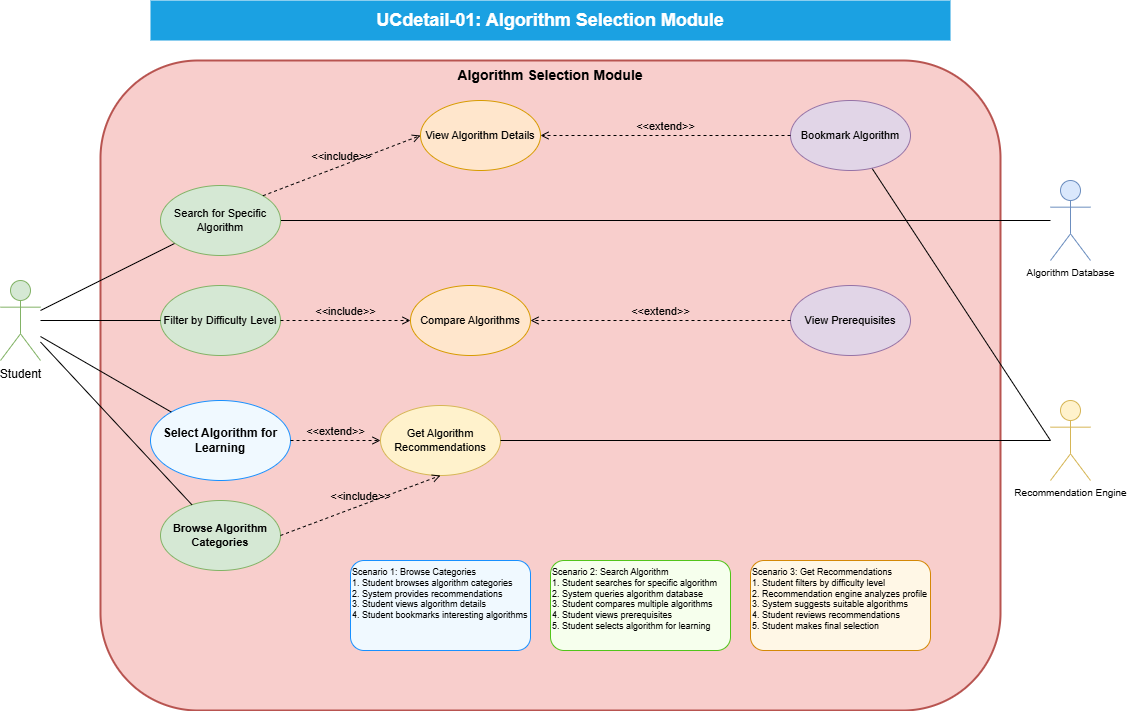
\includegraphics[width=1.0\textwidth]{enhanced-diagrams/UCdetail-01-algorithm-selection.png}
\caption{Sơ đồ Use Case - Tổng quan Hệ thống}
\label{fig:usecase-system-overview}
\end{figure}

\subsection{Phân nhóm Use Case theo Chức năng}
\label{subsec:use-case-functional-groups}

Các use case được tổ chức thành 4 nhóm chức năng chính:

\subsubsection{Nhóm Học Tập Sinh Viên (5 ca sử dụng)}
\begin{enumerate}
    \item \textbf{Học Khái Niệm Thuật Toán}: Học các khái niệm thuật toán cơ bản
    \item \textbf{Thực Hành Với Hình Ảnh Hóa}: Thực hành với animation tương tác
    \item \textbf{Thực Hiện Đánh Giá}: Thực hiện các bài kiểm tra đánh giá
    \item \textbf{Theo Dõi Tiến Độ Học Tập}: Theo dõi tiến độ học tập cá nhân
    \item \textbf{Hợp Tác Với Đồng Học}: Tương tác và học tập cùng đồng học
\end{enumerate}

\subsubsection{Nhóm Quản Lý Giảng Viên (4 ca sử dụng)}
\begin{enumerate}
    \item \textbf{Quản Lý Nội Dung Học Tập}: Quản lý nội dung học tập và tài liệu
    \item \textbf{Tạo Bài Đánh Giá}: Tạo các bài kiểm tra và quiz
    \item \textbf{Theo Dõi Tiến Độ Sinh Viên}: Theo dõi tiến độ học tập của học viên
    \item \textbf{Quản Lý Lớp Học}: Quản lý lớp học và nhóm học viên
\end{enumerate}

\subsubsection{Nhóm Quản Trị Hệ Thống (4 use cases)}
\begin{enumerate}
    \item \textbf{Quản lý Người dùng Hệ thống}: Quản lý tài khoản và quyền người dùng
    \item \textbf{Bảo trì Hệ thống}: Bảo trì và cập nhật hệ thống
    \item \textbf{Giám sát Hiệu suất Hệ thống}: Giám sát hiệu suất hệ thống
    \item \textbf{Quản lý Bảo mật}: Quản lý bảo mật và quyền truy cập
\end{enumerate}
\end{enumerate>

\subsubsection{Nhóm Hỗ trợ Hệ thống Cốt lõi (5 use cases)}
\begin{enumerate}
    \item \textbf{Xác thực Người dùng}: Xác thực và quản lý phiên đăng nhập
    \item \textbf{Quản lý Dữ liệu}: Quản lý dữ liệu và lưu trữ
    \item \textbf{Hỗ trợ AI Thông minh}: Cung cấp hỗ trợ AI thông minh
    \item \textbf{Gửi Thông báo}: Gửi thông báo và cảnh báo
    \item \textbf{Tạo Báo cáo Phân tích}: Tạo báo cáo và phân tích dữ liệu
\end{enumerate}

\subsection{Đặc tả Chi tiết Use Case}
\label{subsec:detailed-usecase-specs}

Phần này trình bày chi tiết các use case chính của hệ thống theo format chuẩn academic, mô tả đầy đủ các luồng sự kiện, điều kiện tiên quyết, và kết quả mong đợi.

\subsubsection{UC001: Học tập Trực quan hóa Thuật toán}

\begin{usecase}
\addheading{Use Case ID}{UC001}
\addrow{Tên Use Case}{Học tập Trực quan hóa Thuật toán}
\addrow{Actor}{Sinh viên}
\addrow{Mô tả ngắn gọn}{Học viên học thuật toán thông qua trực quan hóa tương tác.}
\addrow{Trigger}{Học viên muốn học và hiểu thuật toán thông qua trực quan hóa.}
\addmulrow{Precondition}{\begin{itemize}
    \item Học viên đã đăng nhập vào hệ thống.
    \item Hệ thống có sẵn nội dung thuật toán.
    \item Trình duyệt hỗ trợ HTML5 Canvas/WebGL.
\end{itemize}}
\addmulrow{Main Flow}{\begin{enumerate}
    \item Học viên chọn loại thuật toán muốn học.
    \item Hệ thống hiển thị danh sách thuật toán có sẵn.
    \item Học viên chọn thuật toán cụ thể (VD: Quick Sort).
    \item Hệ thống tải giao diện trực quan hóa thuật toán.
    \item Học viên nhập dữ liệu hoặc sử dụng dữ liệu mẫu.
    \item Học viên bắt đầu quá trình trực quan hóa.
    \item Hệ thống thực hiện hoạt hình từng bước.
    \item Học viên điều khiển tốc độ, tạm dừng, tiếp tục theo nhu cầu.
    \item Hệ thống hiển thị phân tích độ phức tạp và giải thích.
    \item Học viên hoàn thành phiên học tập.
\end{enumerate}}
\addmulrow{Alternative Flow}{\textbf{Alt 1: Học viên muốn so sánh thuật toán}
\begin{itemize}
    \item Từ bước 3, học viên chọn nhiều thuật toán.
    \item Hệ thống hiển thị giao diện so sánh.
    \item Học viên chạy cùng lúc để so sánh hiệu suất.
\end{itemize}}
\addmulrow{Exception Flow}{\textbf{Exc 1: Dữ liệu đầu vào không hợp lệ}
\begin{itemize}
    \item Hệ thống hiển thị thông báo lỗi.
    \item Yêu cầu học viên nhập lại dữ liệu.
\end{itemize}
\textbf{Exc 2: Lỗi thực thi thuật toán}
\begin{itemize}
    \item Hệ thống đặt lại trực quan hóa.
    \item Hiển thị dữ liệu mẫu mặc định.
\end{itemize}}
\addmulrow{Post Condition}{\begin{itemize}
    \item Tiến độ học tập được cập nhật.
    \item Dữ liệu phiên được lưu trong hồ sơ.
    \item Dữ liệu phân tích được ghi nhận.
\end{itemize}}
\end{usecase}

\subsubsection{UC002: Thực hành Thuật toán Tương tác}

\begin{usecase}
\addheading{Use Case ID}{UC002}
\addrow{Tên Use Case}{Thực hành Thuật toán Tương tác}
\addrow{Actor}{Sinh viên}
\addrow{Mô tả ngắn gọn}{Học viên thực hành thuật toán với điều khiển tương tác và đầu vào tùy chỉnh để củng cố kiến thức.}
\addrow{Trigger}{Học viên muốn thực hành và kiểm tra hiểu biết về thuật toán đã học.}
\addmulrow{Precondition}{\begin{itemize}
    \item Học viên đã hoàn thành học tập trực quan hóa cơ bản.
    \item Môi trường thực hành được kích hoạt.
    \item Mẫu thuật toán có sẵn trong hệ thống.
\end{itemize}}
\addmulrow{Main Flow}{\begin{enumerate}
    \item Học viên chọn "Chế độ Thực hành" từ giao diện thuật toán.
    \item Hệ thống hiển thị danh sách thuật toán thực hành có sẵn.
    \item Học viên chọn thuật toán cụ thể để thực hành.
    \item Hệ thống tải môi trường thực hành tương tác với các điều khiển.
    \item Học viên tạo dữ liệu đầu vào tùy chỉnh hoặc chọn từ ví dụ có sẵn.
    \item Học viên dự đoán hành vi thuật toán trước khi thực thi.
    \item Học viên thực thi thuật toán với điều khiển từng bước.
    \item Hệ thống cung cấp phản hồi thời gian thực và gợi ý hiệu suất.
    \item Học viên so sánh dự đoán với kết quả thực thi thực tế.
    \item Hệ thống tính điểm thực hành và cung cấp đề xuất cải thiện.
\end{enumerate}}
\addmulrow{Alternative Flow}{\textbf{Alt 1: Chế độ Thực hành Hướng dẫn}
\begin{itemize}
    \item Hệ thống cung cấp gợi ý và hướng dẫn từng bước.
    \item Học viên được hỗ trợ với giải thích chi tiết cho mỗi bước.
\end{itemize}
\textbf{Alt 2: Chế độ Thực hành Thách thức}
\begin{itemize}
    \item Hệ thống đưa ra thách thức cụ thể với giới hạn thời gian.
    \item Học viên phải hoàn thành nhiệm vụ trong giới hạn thời gian.
\end{itemize}}
\addmulrow{Exception Flow}{\textbf{Exc 1: Dữ liệu đầu vào thực hành không hợp lệ}
\begin{itemize}
    \item Hệ thống xác thực đầu vào và hiển thị thông báo lỗi cụ thể.
    \item Cung cấp ví dụ đầu vào hợp lệ được đề xuất và hướng dẫn định dạng.
\end{itemize}
\textbf{Exc 2: Phiên thực hành hết thời gian}
\begin{itemize}
    \item Hệ thống tự động lưu tiến độ và trạng thái hiện tại.
    \item Cho phép học viên tiếp tục từ điểm lưu đã lưu.
\end{itemize}}
\addmulrow{Post Condition}{\begin{itemize}
    \item Điểm hiệu suất thực hành được ghi lại vào hồ sơ người dùng.
    \item Chỉ số đánh giá kỹ năng được cập nhật dựa trên hiệu suất.
    \item Huy hiệu thành tựu có thể được mở khóa.
    \item Lịch sử thực hành được lưu để tham khảo và xem xét trong tương lai.
\end{itemize}}
\end{usecase}

\subsubsection{UC003: Tư vấn Trợ lý AI}

\begin{usecase}
\addheading{Use Case ID}{UC003}
\addrow{Tên Use Case}{Tư vấn Trợ lý AI}
\addrow{Actor}{Sinh viên}
\addrow{Mô tả ngắn gọn}{Học viên tương tác với Trợ lý AI để nhận hỗ trợ học tập thông minh và giải đáp thắc mắc.}
\addrow{Trigger}{Học viên gặp khó khăn hoặc cần giải thích chi tiết về các khái niệm thuật toán.}
\addmulrow{Precondition}{\begin{itemize}
    \item Học viên đang trong phiên học tập hoạt động.
    \item Dịch vụ Trợ lý AI đang có sẵn và phản hồi.
    \item Kết nối mạng ổn định cho tương tác thời gian thực.
    \item Bối cảnh học tập hiện tại được tải thành công.
\end{itemize}}
\addmulrow{Main Flow}{\begin{enumerate}
    \item Học viên nhấp vào biểu tượng Trợ lý AI trong giao diện học tập.
    \item Hệ thống mở giao diện trò chuyện AI với tải bối cảnh hiện tại.
    \item Học viên nhập câu hỏi về thuật toán hiện tại hoặc các khái niệm liên quan.
    \item Trợ lý AI phân tích bối cảnh câu hỏi và nhận dạng ý định.
    \item AI tạo phản hồi toàn diện với ví dụ và giải thích.
    \item Hệ thống hiển thị câu trả lời AI với định dạng phù hợp và tô sáng mã.
    \item Học viên có thể đặt câu hỏi tiếp theo để làm rõ thắc mắc.
    \item AI cung cấp tài nguyên học tập bổ sung và gợi ý nếu phù hợp.
    \item Học viên đóng Trợ lý AI khi hài lòng với câu trả lời.
    \item Hệ thống lưu lịch sử cuộc trò chuyện để tham khảo trong tương lai.
\end{enumerate}}
\addmulrow{Alternative Flow}{\textbf{Alt 1: Code Analysis Request}
\begin{itemize}
    \item Học viên paste existing code snippet để AI review.
    \item AI analyze code quality và suggest optimizations với detailed explanations.
\end{itemize}
\textbf{Alt 2: Algorithm Recommendation}
\begin{itemize}
    \item Học viên describe specific problem cần solve.
    \item AI recommend suitable algorithms với pros/cons comparison.
\end{itemize}
\textbf{Alt 3: Step-by-step Explanation}
\begin{itemize}
    \item Học viên request explanation cho current visualization step.
    \item AI provide synchronized explanation với animation context.
\end{itemize}}
\addmulrow{Exception Flow}{\textbf{Exc 1: Dịch vụ AI tạm thời không khả dụng}
\begin{itemize}
    \item Hệ thống hiển thị tài nguyên dự phòng và tài liệu tĩnh.
    \item Chuyển hướng đến FAQ hoặc cơ sở kiến thức cộng đồng.
    \item Ghi nhận sự cố cho giám sát dịch vụ.
\end{itemize}
\textbf{Exc 2: Câu hỏi quá phức tạp hoặc mơ hồ}
\begin{itemize}
    \item AI yêu cầu làm rõ với các câu hỏi hướng dẫn cụ thể.
    \item Gợi ý chia nhỏ câu hỏi phức tạp thành các phần nhỏ hơn.
\end{itemize}
\textbf{Exc 3: Vượt quá giới hạn tốc độ truy cập}
\begin{itemize}
    \item Hiển thị thông báo giới hạn tốc độ với bộ đếm thời gian.
    \item Gợi ý tài nguyên trợ giúp thay thế trong thời gian chờ.
\end{itemize}}
\addmulrow{Post Condition}{\begin{itemize}
    \item Lịch sử cuộc trò chuyện được lưu trong hồ sơ học tập của người dùng.
    \item Dữ liệu tương tác AI góp phần cải thiện mô hình.
    \item Phản hồi hài lòng của người dùng được thu thập tự động.
    \item Tài liệu học tập liên quan được gợi ý dựa trên mẫu tương tác.
    \item Phân tích học tập được cập nhật với chỉ số sử dụng AI.
\end{itemize}}
\end{usecase}

\subsubsection{UC004: Phân tích So sánh Thuật toán}

\begin{usecase}
\addheading{Use Case ID}{UC004}
\addrow{Tên Use Case}{Phân tích So sánh Thuật toán}
\addrow{Actor}{Sinh viên}
\addrow{Mô tả ngắn gọn}{Học viên so sánh hiệu suất và đặc điểm của nhiều thuật toán cùng lúc.}
\addrow{Trigger}{Học viên muốn hiểu sự khác biệt và sự đánh đổi giữa các thuật toán.}
\addmulrow{Precondition}{\begin{itemize}
    \item Ít nhất 2 thuật toán có sẵn cho việc so sánh.
    \item Giao diện so sánh được hỗ trợ bởi trình duyệt.
    \item Dữ liệu đầu vào tương thích với tất cả thuật toán được chọn.
\end{itemize}}
\addmulrow{Main Flow}{\begin{enumerate}
    \item Học viên chọn "So sánh Thuật toán" từ thư viện thuật toán.
    \item Hệ thống hiển thị giao diện lựa chọn cho nhiều thuật toán.
    \item Học viên chọn 2-4 thuật toán để so sánh (VD: Sắp xếp Nổi bọt vs Sắp xếp Nhanh vs Sắp xếp Trộn).
    \item Hệ thống tải giao diện so sánh với khung nhìn song song.
    \item Học viên cấu hình dữ liệu đầu vào chung cho tất cả thuật toán.
    \item Học viên bắt đầu thực thi đồng thời của tất cả thuật toán.
    \item Hệ thống chạy thuật toán đồng thời với trực quan hóa đồng bộ.
    \item Hiển thị chỉ số hiệu suất thời gian thực: độ phức tạp thời gian, sử dụng không gian, số bước.
    \item Học viên có thể điều chỉnh tốc độ thực thi và tạm dừng/tiếp tục tất cả thuật toán.
    \item Hệ thống trình bày kết quả so sánh cuối cùng với phân tích thống kê.
\end{enumerate}}
\addmulrow{Alternative Flow}{\textbf{Alt 1: So sánh Kích thước Đầu vào Khác nhau}
\begin{itemize}
    \item Học viên chọn nhiều kích thước đầu vào để kiểm tra khả năng mở rộng.
    \item Hệ thống chạy thuật toán với các kích thước tập dữ liệu khác nhau.
    \item Hiển thị biểu đồ tỷ lệ hiệu suất và phân tích độ phức tạp.
\end{itemize}
\textbf{Alt 2: Phân tích Trường hợp Tốt nhất/Xấu nhất}
\begin{itemize}
    \item Học viên chọn các trường hợp kiểm tra cụ thể: tốt nhất, trung bình, xấu nhất.
    \item Hệ thống tạo dữ liệu đầu vào phù hợp cho từng tình huống.
\end{itemize}}
\addmulrow{Exception Flow}{\textbf{Exc 1: Lựa chọn thuật toán không tương thích}
\begin{itemize}
    \item Hệ thống phát hiện thuật toán không thể so sánh trực tiếp.
    \item Gợi ý thuật toán thay thế hoặc cung cấp giải thích về sự không tương thích.
\end{itemize}
\textbf{Exc 2: Lỗi đo lường hiệu suất}
\begin{itemize}
    \item Hệ thống thử lại đo lường với tham số đã điều chỉnh.
    \item Cung cấp kết quả gần đúng với khoảng tin cậy.
\end{itemize}}
\addmulrow{Post Condition}{\begin{itemize}
    \item Kết quả so sánh được lưu trong lịch sử học tập của người dùng.
    \item Điểm chuẩn hiệu suất đóng góp vào phân tích hệ thống.
    \item Đánh giá hiểu biết được cập nhật dựa trên thông tin so sánh.
    \item Tài nguyên học tập liên quan được gợi ý để hiểu sâu hơn.
\end{itemize}}
\end{usecase}

\subsubsection{UC005: Theo dõi Tiến độ Học tập}

\begin{usecase}
\addheading{Use Case ID}{UC005}
\addrow{Tên Use Case}{Theo dõi Tiến độ Học tập}
\addrow{Actor}{Sinh viên}
\addrow{Mô tả ngắn gọn}{Học viên theo dõi và xem xét tiến độ học tập với phân tích chi tiết và khuyến nghị.}
\addrow{Trigger}{Học viên muốn xem xét thành tích học tập và lập kế hoạch cho các bước học tiếp theo.}
\addmulrow{Precondition}{\begin{itemize}
    \item Học viên đã có ít nhất một phiên học tập được hoàn thành.
    \item Dịch vụ theo dõi tiến độ đang hoạt động bình thường.
    \item Dữ liệu hồ sơ người dùng có thể truy cập và cập nhật.
\end{itemize}}
\addmulrow{Main Flow}{\begin{enumerate}
    \item Học viên truy cập bảng điều khiển "Tiến độ của Tôi" từ thanh điều hướng chính.
    \item Hệ thống tải dữ liệu tiến độ toàn diện và phân tích.
    \item Hiển thị thống kê học tập tổng thể: thuật toán đã hoàn thành, thời gian học, mức độ kỹ năng.
    \item Hiển thị phân tích chi tiết theo danh mục thuật toán và mức độ khó.
    \item Trình bày quỹ đạo học tập với biểu đồ tiến độ theo thời gian.
    \item Hiển thị huy hiệu thành tích đã đạt được và các cột mốc đã đạt tới.
    \item Hiển thị khuyến nghị cá nhân hóa cho các mục tiêu học tập tiếp theo.
    \item Học viên có thể xem chi tiết hiệu suất thuật toán cụ thể.
    \item Xem xét điểm thực hành và kết quả đánh giá với phân tích xu hướng.
    \item Đặt mục tiêu học tập và chỉ tiêu cho các phiên học sắp tới.
\end{enumerate}}
\addmulrow{Alternative Flow}{\textbf{Alt 1: So sánh với Hiệu suất Đồng nghiệp}
\begin{itemize}
    \item Học viên kích hoạt tính năng so sánh đồng nghiệp ẩn danh.
    \item Hệ thống hiển thị chỉ số hiệu suất tương đối so với mức trung bình lớp/nhóm.
\end{itemize}
\textbf{Alt 2: Phân tích Thời gian Chi tiết}
\begin{itemize}
    \item Học viên yêu cầu phân tích chi tiết về thời gian sử dụng.
    \item Hiển thị phân bổ thời gian qua các hoạt động học tập khác nhau.
\end{itemize}
\textbf{Alt 3: Xuất Báo cáo Tiến độ}
\begin{itemize}
    \item Học viên yêu cầu báo cáo tiến độ có thể tải về.
    \item Hệ thống tạo báo cáo PDF với phân tích toàn diện.
\end{itemize}}
\addmulrow{Exception Flow}{\textbf{Exc 1: Dữ liệu tiến độ không đủ}
\begin{itemize}
    \item Hệ thống thông báo về yêu cầu dữ liệu tối thiểu.
    \item Gợi ý hoàn thành nhiều hoạt động học tập hơn để mở khóa phân tích đầy đủ.
\end{itemize}
\textbf{Exc 2: Dịch vụ phân tích không khả dụng}
\begin{itemize}
    \item Hiển thị dữ liệu tiến độ đã lưu với chỉ báo thời gian.
    \item Lên lịch làm mới tự động khi dịch vụ khả dụng trở lại.
\end{itemize}}
\addmulrow{Post Condition}{\begin{itemize}
    \item Hoạt động xem xét tiến độ được ghi lại cho phân tích sử dụng.
    \item Mục tiêu và chỉ tiêu học tập được lưu trong hồ sơ người dùng.
    \item Bộ máy khuyến nghị được cập nhật với mẫu tương tác người dùng.
    \item Chỉ số động lực được tính toán dựa trên tần suất xem xét tiến độ.
\end{itemize}}
\end{usecase}

\subsubsection{UC006: Quản lý Người dùng}

\begin{usecase}
\addheading{Use Case ID}{UC006}
\addrow{Tên Use Case}{Quản lý Tài khoản Người dùng}
\addrow{Actor}{Sinh viên, Giảng viên, Quản trị viên}
\addrow{Mô tả ngắn gọn}{Quản lý tài khoản người dùng bao gồm đăng ký, đăng nhập, quản lý hồ sơ và phân quyền.}
\addrow{Trigger}{Người dùng cần tạo tài khoản hoặc truy cập hệ thống.}
\addmulrow{Precondition}{\begin{itemize}
    \item Dịch vụ xác thực hệ thống hoạt động
    \item Cơ sở dữ liệu quản lý người dùng khả dụng
    \item Dịch vụ email kết nối thành công
\end{itemize}}
\addmulrow{Main Flow}{\begin{enumerate}
    \item Người dùng truy cập trang đăng ký/đăng nhập
    \item Hệ thống hiển thị biểu mẫu xác thực với xác nhận
    \item Người dùng nhập thông tin tài khoản (email, mật khẩu, vai trò)
    \item Hệ thống xác nhận thông tin và kiểm tra email trùng lặp
    \item Hệ thống tạo tài khoản người dùng với mật khẩu được mã hóa
    \item Hệ thống gửi email xác nhận để kích hoạt tài khoản
    \item Người dùng nhấp vào liên kết xác nhận từ email
    \item Hệ thống kích hoạt tài khoản và chuyển hướng đến bảng điều khiển
    \item Hệ thống ghi lại hoạt động người dùng và cập nhật thời gian đăng nhập cuối
\end{enumerate}}
\addmulrow{Alternative Flow}{\begin{itemize}
    \item Email đã tồn tại: Hệ thống hiển thị thông báo lỗi và gợi ý đăng nhập
    \item Gửi email xác nhận thất bại: Hệ thống cung cấp tùy chọn gửi lại xác nhận
    \item Mật khẩu không đạt yêu cầu: Hệ thống hiển thị chỉ báo độ mạnh mật khẩu
    \item Đăng nhập xã hội: Người dùng có thể đăng nhập qua Google/GitHub OAuth
\end{itemize}}
\addmulrow{Exception Flow}{\begin{itemize}
    \item Dịch vụ email không khả dụng: Cho phép kích hoạt thủ công bởi quản trị viên
    \item Cơ sở dữ liệu không kết nối được: Hiển thị thông báo lỗi hệ thống
    \item Xác thực OAuth thất bại: Quay về phương thức đăng nhập truyền thống
\end{itemize}}
\addmulrow{Post Condition}{\begin{itemize}
    \item Tài khoản người dùng được tạo và kích hoạt thành công
    \item Phiên người dùng được thiết lập với quyền phù hợp
    \item Dữ liệu hồ sơ người dùng được khởi tạo với cài đặt mặc định
    \item Hệ thống tạo không gian làm việc người dùng và theo dõi tiến độ học tập
\end{itemize}}
\end{usecase}

\subsubsection{UC007: Học tập Hợp tác}

\begin{usecase}
\addheading{Use Case ID}{UC007}
\addrow{Tên Use Case}{Môi trường Học tập Hợp tác}
\addrow{Actor}{Sinh viên, Giảng viên}
\addrow{Mô tả ngắn gọn}{Tạo môi trường học tập hợp tác với chia sẻ, thảo luận, và đánh giá đồng nghiệp.}
\addrow{Trigger}{Người dùng muốn học tập theo nhóm hoặc chia sẻ kiến thức.}
\addmulrow{Precondition}{\begin{itemize}
    \item Người dùng đã đăng nhập với quyền phù hợp
    \item Dịch vụ truyền thông thời gian thực hoạt động
    \item Hệ thống thông báo khả dụng
\end{itemize}}
\addmulrow{Main Flow}{\begin{enumerate}
    \item Người dùng tạo hoặc tham gia nhóm học tập/lớp học
    \item Hệ thống thiết lập không gian làm việc chung với công cụ hợp tác
    \item Người dùng chia sẻ phiên trực quan hóa với thành viên nhóm
    \item Hệ thống cho phép chia sẻ mã và thảo luận thời gian thực
    \item Thành viên có thể bình luận, đề xuất cải tiến về thuật toán
    \item Hệ thống theo dõi hoạt động hợp tác và đóng góp
    \item Giảng viên có thể giám sát tiến độ nhóm và cung cấp hướng dẫn
    \item Hệ thống tạo báo cáo hợp tác và đánh giá đồng nghiệp
    \item Người dùng nhận thông báo về hoạt động và cập nhật nhóm
\end{enumerate}}
\addmulrow{Alternative Flow}{\begin{itemize}
    \item Phiên học tập riêng tư: Người dùng có thể làm việc độc lập nếu muốn
    \item Chế độ ngoại tuyến: Hệ thống lưu trữ dữ liệu hợp tác để đồng bộ sau
    \item Xung đột quyền: Hệ thống giải quyết quyền truy cập theo thứ bậc vai trò
    \item Vấn đề mạng: Hệ thống cung cấp tính năng hợp tác ngoại tuyến
\end{itemize}}
\addmulrow{Exception Flow}{\begin{itemize}
    \item Mất kết nối thời gian thực: Chuyển sang chế độ bình luận bất đồng bộ
    \item Xung đột chỉnh sửa: Hiển thị thông báo và cho phép giải quyết thủ công
    \item Quá tải hệ thống: Giới hạn số lượng thành viên đồng thời
\end{itemize}}
\addmulrow{Post Condition}{\begin{itemize}
    \item Phiên hợp tác được thiết lập thành công
    \item Tất cả người tham gia có quyền truy cập vào tài nguyên chung
    \item Đồng bộ hóa thời gian thực hoạt động đúng cách
    \item Lịch sử hợp tác được lưu để tham khảo trong tương lai
\end{itemize}}
\end{usecase}

\subsubsection{UC008: Trợ lý Học tập Thông minh AI}

\begin{usecase}
\addheading{Use Case ID}{UC008}
\addrow{Tên Use Case}{Trợ lý Học tập Thông minh AI}
\addrow{Actor}{Sinh viên, Giảng viên}
\addrow{Mô tả ngắn gọn}{Trợ lý AI cung cấp hỗ trợ học tập cá nhân hóa, giải thích thuật toán, và khuyến nghị.}
\addrow{Trigger}{Người dùng cần hỗ trợ hoặc giải thích về thuật toán.}
\addmulrow{Precondition}{\begin{itemize}
    \item Mô hình dịch vụ AI đã được huấn luyện và triển khai
    \item Lịch sử học tập và tùy chọn người dùng có sẵn
    \item Cơ sở kiến thức được cập nhật với thuật toán hiện tại
\end{itemize}}
\addmulrow{Main Flow}{\begin{enumerate}
    \item Người dùng gửi truy vấn hoặc yêu cầu trợ giúp về thuật toán cụ thể
    \item Trợ lý AI phân tích câu hỏi người dùng và bối cảnh học tập hiện tại
    \item Hệ thống truy xuất thông tin liên quan từ cơ sở kiến thức
    \item AI tạo giải thích cá nhân hóa với mức độ phức tạp phù hợp
    \item Hệ thống cung cấp ví dụ tương tác và minh họa trực quan
    \item AI gợi ý thuật toán liên quan và lộ trình học tập
    \item Người dùng có thể đặt câu hỏi tiếp theo để làm rõ khái niệm
    \item Hệ thống cập nhật hồ sơ học tập người dùng dựa trên tương tác
    \item AI khuyến nghị các bước học tập tiếp theo và bài tập thực hành
\end{enumerate}}
\addmulrow{Alternative Flow}{\begin{itemize}
    \item Truy vấn phức tạp: AI chuyển giao cho giảng viên con người nếu cần
    \item Hỗ trợ đa ngôn ngữ: AI có thể phản hồi bằng ngôn ngữ ưa thích
    \item Thích ứng phong cách học tập: AI điều chỉnh phong cách giải thích theo tùy chọn người dùng
    \item Gỡ lỗi mã: AI phân tích mã người dùng và gợi ý cải tiến
\end{itemize}}
\addmulrow{Exception Flow}{\begin{itemize}
    \item Dịch vụ AI không khả dụng: Chuyển hướng đến tài liệu hướng dẫn tĩnh
    \item Câu hỏi ngoài phạm vi: AI thông báo giới hạn và gợi ý nguồn thay thế
    \item Quá tải hệ thống: Xếp hàng đợi yêu cầu và thông báo thời gian chờ
\end{itemize}}
\addmulrow{Post Condition}{\begin{itemize}
    \item Người dùng nhận được giải thích chính xác và hữu ích
    \item Tiến độ học tập được cập nhật với dữ liệu tương tác AI
    \item Mô hình AI được huấn luyện lại với phản hồi người dùng
    \item Khuyến nghị cá nhân hóa được tạo cho việc học tương lai
\end{itemize}}
\end{usecase}

\subsubsection{UC009: Hệ thống Quản lý Nội dung}

\begin{usecase}
\addheading{Use Case ID}{UC009}
\addrow{Tên Use Case}{Hệ thống Quản lý Nội dung Động}
\addrow{Actor}{Giảng viên, Quản trị viên Nội dung}
\addrow{Mô tả ngắn gọn}{Quản lý nội dung học tập động bao gồm thuật toán, bài tập, và tài liệu giáo dục.}
\addrow{Trigger}{Giảng viên cần tạo hoặc cập nhật nội dung học tập.}
\addmulrow{Precondition}{\begin{itemize}
    \item Người dùng có quyền quản lý nội dung
    \item Hệ thống quản lý nội dung hoạt động đúng cách
    \item Dịch vụ kiểm soát phiên bản khả dụng
\end{itemize}}
\addmulrow{Main Flow}{\begin{enumerate}
    \item Giảng viên truy cập bảng điều khiển quản lý nội dung
    \item Hệ thống hiển thị thư viện nội dung hiện có với tùy chọn tìm kiếm/lọc
    \item Giảng viên tạo nội dung thuật toán mới hoặc chỉnh sửa nội dung hiện có
    \item Hệ thống cung cấp trình soạn thảo văn bản phong phú với tô sáng mã
    \item Giảng viên thêm tham số trực quan hóa và phần tử tương tác
    \item Hệ thống xác nhận định dạng nội dung và tính đúng đắn của thuật toán
    \item Giảng viên thiết lập bài tập và câu hỏi đánh giá
    \item Hệ thống xem trước nội dung với các mức độ phức tạp khác nhau
    \item Giảng viên xuất bản nội dung sau khi xem xét và phê duyệt
    \item Hệ thống cập nhật chỉ mục nội dung và thông báo cho người dùng liên quan
\end{enumerate}}
\addmulrow{Alternative Flow}{\begin{itemize}
    \item Nhập nội dung: Giảng viên có thể nhập từ nguồn bên ngoài
    \item Chỉnh sửa hợp tác: Nhiều giảng viên có thể hợp tác trên cùng nội dung
    \item Phiên bản nội dung: Hệ thống duy trì lịch sử phiên bản để khôi phục nếu cần
    \item Thao tác hàng loạt: Hệ thống hỗ trợ tải lên và chỉnh sửa hàng loạt
\end{itemize}}
\addmulrow{Exception Flow}{\begin{itemize}
    \item Lỗi xác thực nội dung: Hiển thị thông báo lỗi chi tiết và gợi ý sửa chữa
    \item Xung đột phiên bản: Cung cấp công cụ hợp nhất thay đổi
    \item Dung lượng vượt quá: Nén hoặc đề xuất tối ưu hóa nội dung
\end{itemize}}
\addmulrow{Post Condition}{\begin{itemize}
    \item Nội dung mới được xuất bản và có sẵn cho người dùng
    \item Siêu dữ liệu nội dung được lập chỉ mục đúng cách để tìm kiếm
    \item Lịch sử phiên bản được duy trì để theo dõi nội dung
    \item Người dùng liên quan nhận thông báo về nội dung mới
\end{itemize}}
\end{usecase}

\subsubsection{UC010: Quản trị Hệ thống}

\begin{usecase}
\addheading{Use Case ID}{UC010}
\addrow{Tên Use Case}{Quản trị Hệ thống và Giám sát}
\addrow{Actor}{Quản trị viên Hệ thống, Kỹ sư DevOps}
\addrow{Mô tả ngắn gọn}{Quản lý hệ thống toàn diện bao gồm giám sát, bảo trì, và quản lý bảo mật.}
\addrow{Trigger}{Cần thực hiện giám sát, bảo trì, hoặc quản lý hệ thống.}
\addmulrow{Precondition}{\begin{itemize}
    \item Quản trị viên có đặc quyền truy cập hệ thống đầy đủ
    \item Công cụ giám sát và bảng điều khiển hoạt động
    \item Hệ thống sao lưu được cấu hình đúng cách
\end{itemize}}
\addmulrow{Main Flow}{\begin{enumerate}
    \item Quản trị viên truy cập bảng điều khiển quản trị hệ thống
    \item Hệ thống hiển thị chỉ số thời gian thực: hiệu suất, sử dụng, lỗi
    \item Quản trị viên giám sát hoạt động người dùng và tình trạng hệ thống
    \item Hệ thống tạo báo cáo tự động về mẫu sử dụng
    \item Quản trị viên thực hiện các tác vụ bảo trì thường xuyên
    \item Hệ thống sao lưu dữ liệu và cấu hình quan trọng
    \item Quản trị viên xem xét nhật ký bảo mật và mẫu truy cập
    \item Hệ thống thực hiện quét bảo mật và đánh giá lỗ hổng
    \item Quản trị viên cập nhật cấu hình và chính sách hệ thống
    \item Hệ thống thông báo cho các bên liên quan về hoạt động bảo trì
\end{enumerate}}
\addmulrow{Alternative Flow}{\begin{itemize}
    \item Phản ứng khẩn cấp: Hệ thống kích hoạt cảnh báo cho các vấn đề nghiêm trọng
    \item Bảo trì tự động: Hệ thống thực hiện các tác vụ đã lên lịch tự động
    \item Tối ưu hóa hiệu suất: Quản trị viên điều chỉnh tham số hệ thống
    \item Khôi phục thảm họa: Hệ thống thực thi quy trình khôi phục sao lưu
\end{itemize}}
\addmulrow{Exception Flow}{\begin{itemize}
    \item Lỗi hệ thống nghiêm trọng: Kích hoạt chế độ khẩn cấp và thông báo ngay lập tức
    \item Sao lưu thất bại: Thực hiện sao lưu thủ công và kiểm tra hệ thống lưu trữ
    \item Tấn công bảo mật: Kích hoạt giao thức bảo mật và cách ly hệ thống bị ảnh hưởng
\end{itemize}}
\addmulrow{Post Condition}{\begin{itemize}
    \item Chỉ số tình trạng hệ thống trong phạm vi chấp nhận được
    \item Chính sách bảo mật được thực thi đúng cách
    \item Dữ liệu sao lưu được xác minh và có thể truy cập
    \item Hiệu suất hệ thống được tối ưu hóa cho trải nghiệm người dùng
\end{itemize}}
\end{usecase}

\section{Biểu đồ Lớp}
\label{sec:class-diagram}

\subsection{Tổng quan Biểu đồ Lớp}
\label{subsec:class-overview}

Biểu đồ lớp của hệ thống DSA Visualizer được thiết kế theo mô hình MVC (Model-View-Controller) và Clean Architecture, đảm bảo tính modular và scalability.

\begin{center}
\textbf{[Biểu đồ Lớp - Hệ thống Cốt lõi]}\\
\textit{Diagram: class-diagram-clean.drawio}
\end{center}

\subsection{Các nhóm Lớp chính}

\subsubsection{Các Lớp Quản lý Người dùng}

\textbf{Lớp User:}
\begin{itemize}
    \item \textbf{Thuộc tính:} userID, email, username, password, role, createdAt, lastLogin
    \item \textbf{Phương thức:} login(), logout(), updateProfile(), changePassword()
    \item \textbf{Mối quan hệ:} User có nhiều LearningSession, có một UserProfile
\end{itemize}

\textbf{Lớp UserProfile:}
\begin{itemize}
    \item \textbf{Thuộc tính:} profileID, firstName, lastName, avatar, bio, preferences
    \item \textbf{Phương thức:} updatePersonalInfo(), setPreferences(), uploadAvatar()
    \item \textbf{Mối quan hệ:} Thuộc về một User, có nhiều Achievement
\end{itemize}

\subsubsection{Các Lớp Trực quan hóa Thuật toán}

\textbf{Lớp Algorithm:}
\begin{itemize}
    \item \textbf{Thuộc tính:} algorithmID, name, category, description, complexity, difficulty
    \item \textbf{Phương thức:} execute(), visualize(), getComplexity(), generateSteps()
    \item \textbf{Mối quan hệ:} Có nhiều AlgorithmStep, thuộc về một Category
\end{itemize}

\textbf{Lớp Visualizer:}
\begin{itemize}
    \item \textbf{Thuộc tính:} visualizerID, type, config, animationSpeed, currentStep
    \item \textbf{Phương thức:} start(), pause(), resume(), reset(), setSpeed()
    \item \textbf{Mối quan hệ:} Sử dụng Algorithm, tạo ra VisualizationSession
\end{itemize}

\textbf{Lớp AlgorithmStep:}
\begin{itemize}
    \item \textbf{Thuộc tính:} stepID, stepNumber, description, dataState, action
    \item \textbf{Phương thức:} execute(), undo(), getDescription(), visualize()
    \item \textbf{Mối quan hệ:} Thuộc về một Algorithm
\end{itemize}

\subsubsection{Các Lớp Quản lý Học tập}

\textbf{Lớp LearningSession:}
\begin{itemize}
    \item \textbf{Thuộc tính:} sessionID, userID, algorithmID, startTime, endTime, score
    \item \textbf{Phương thức:} start(), complete(), calculateScore(), saveProgress()
    \item \textbf{Mối quan hệ:} Thuộc về User và Algorithm
\end{itemize}

\textbf{Lớp Progress:}
\begin{itemize}
    \item \textbf{Thuộc tính:} progressID, userID, totalSessions, completedAlgorithms, skillLevel
    \item \textbf{Phương thức:} updateProgress(), calculateSkillLevel(), getStatistics()
    \item \textbf{Mối quan hệ:} Thuộc về một User
\end{itemize}

\subsubsection{Các Lớp Đánh giá}

\textbf{Lớp Quiz:}
\begin{itemize}
    \item \textbf{Thuộc tính:} quizID, title, description, questions, timeLimit, difficulty
    \item \textbf{Phương thức:} generateQuestions(), calculateScore(), validateAnswers()
    \item \textbf{Mối quan hệ:} Có nhiều Question, có nhiều QuizResult
\end{itemize}

\textbf{Lớp Question:}
\begin{itemize}
    \item \textbf{Thuộc tính:} questionID, content, options, correctAnswer, explanation
    \item \textbf{Phương thức:} validateAnswer(), getHint(), getExplanation()
    \item \textbf{Mối quan hệ:} Thuộc về một Quiz
\end{itemize}

\subsection{Các Mẫu Thiết kế được sử dụng}

\subsubsection{Mẫu Factory Pattern}
Sử dụng AlgorithmFactory để tạo ra các thể hiện của các loại thuật toán khác nhau:
\begin{itemize}
    \item SortingAlgorithmFactory
    \item SearchAlgorithmFactory  
    \item GraphAlgorithmFactory
\end{itemize}

\subsubsection{Mẫu Observer Pattern}
VisualizationObserver được thực hiện để thông báo cho các thành phần UI khi trạng thái thuật toán thay đổi:
\begin{itemize}
    \item ProgressObserver: Cập nhật thanh tiến độ
    \item AnimationObserver: Kích hoạt hiệu ứng hoạt hình
    \item ScoreObserver: Tính toán và hiển thị điểm số
\end{itemize}

\subsubsection{Mẫu Strategy Pattern}
Sử dụng cho các chiến lược thực thi thuật toán:
\begin{itemize}
    \item StepByStepStrategy: Thực thi từng bước
    \item ContinuousStrategy: Thực thi liên tục
    \item ComparisonStrategy: So sánh nhiều thuật toán
\end{itemize}

\section{Biểu đồ Hoạt động}
\label{sec:activity-diagram}

\subsection{Tổng quan Biểu đồ Hoạt động}
\label{subsec:activity-overview}

Biểu đồ hoạt động mô tả luồng hoạt động chính của hệ thống, từ khi người dùng đăng nhập cho đến khi hoàn thành phiên học tập.

\begin{center}
\textbf{[Biểu đồ Hoạt động - Quy trình Học tập]}\\
\textit{Diagram: activity-diagram-clean.drawio}
\end{center}

\subsection{Quy trình hoạt động chính}

\subsubsection{Luồng Xác thực}
\begin{enumerate}
    \item \textbf{Bắt đầu:} Người dùng truy cập ứng dụng
    \item \textbf{Quyết định:} Kiểm tra người dùng đã đăng nhập chưa?
    \item \textbf{Sai:} Chuyển hướng đến trang đăng nhập
    \item \textbf{Quy trình Đăng nhập:} Người dùng nhập thông tin đăng nhập
    \item \textbf{Xác nhận:} Hệ thống xác nhận thông tin người dùng
    \item \textbf{Quyết định:} Thông tin đăng nhập có hợp lệ?
    \item \textbf{Sai:} Hiển thị thông báo lỗi, quay lại đăng nhập
    \item \textbf{Đúng:} Tạo JWT token, chuyển hướng đến bảng điều khiển
\end{enumerate}

\subsubsection{Luồng Học tập Thuật toán}
\begin{enumerate}
    \item \textbf{Truy cập Bảng điều khiển:} Người dùng vào bảng điều khiển chính
    \item \textbf{Lựa chọn Danh mục:} Người dùng chọn danh mục thuật toán
    \item \textbf{Lựa chọn Thuật toán:} Người dùng chọn thuật toán cụ thể
    \item \textbf{Tải Trực quan hóa:} Hệ thống tải trình trực quan hóa thuật toán
    \item \textbf{Cấu hình Đầu vào:} Người dùng cấu hình dữ liệu đầu vào
    \item \textbf{Quyết định:} Người dùng muốn bắt đầu trực quan hóa?
    \item \textbf{Đúng:} Bắt đầu thực thi thuật toán
    \item \textbf{Thực thi Từng bước:} Hệ thống thực thi từng bước
    \item \textbf{Hiển thị Hoạt hình:} Hiển thị hoạt hình trực quan
    \item \textbf{Tương tác Người dùng:} Người dùng có thể tạm dừng/tiếp tục/điều chỉnh tốc độ
    \item \textbf{Kiểm tra Hoàn thành:} Thực thi thuật toán hoàn thành?
    \item \textbf{Sai:} Tiếp tục bước tiếp theo
    \item \textbf{Đúng:} Hiển thị kết quả cuối cùng và phân tích độ phức tạp
\end{enumerate}

\subsubsection{Luồng Trợ lý AI}
\begin{enumerate}
    \item \textbf{Kích hoạt:} Người dùng nhấp nút Trợ lý AI
    \item \textbf{Thu thập Bối cảnh:} Hệ thống thu thập bối cảnh học tập hiện tại
    \item \textbf{Nhập Câu hỏi:} Người dùng nhập câu hỏi
    \item \textbf{Xử lý NLP:} AI phân tích ý định câu hỏi
    \item \textbf{Truy xuất Kiến thức:} AI tìm kiếm thông tin liên quan
    \item \textbf{Tạo Phản hồi:} AI tạo phản hồi phù hợp
    \item \textbf{Hiển thị Phản hồi:} Hệ thống hiển thị phản hồi AI
    \item \textbf{Quyết định:} Người dùng có câu hỏi bổ sung?
    \item \textbf{Đúng:} Quay lại nhập câu hỏi
    \item \textbf{Sai:} Đóng Trợ lý AI
\end{enumerate}

\subsubsection{Luồng Đánh giá}
\begin{enumerate}
    \item \textbf{Lựa chọn Bài kiểm tra:} Người dùng chọn bài kiểm tra để làm
    \item \textbf{Tải Bài kiểm tra:} Hệ thống tải câu hỏi bài kiểm tra
    \item \textbf{Hiển thị Câu hỏi:} Hiển thị câu hỏi hiện tại
    \item \textbf{Nhập Câu trả lời:} Người dùng chọn/nhập câu trả lời
    \item \textbf{Xác nhận Câu trả lời:} Hệ thống xác nhận câu trả lời
    \item \textbf{Hiển thị Phản hồi:} Hiển thị phản hồi ngay lập tức
    \item \textbf{Cập nhật Tiến độ:} Cập nhật tiến độ bài kiểm tra
    \item \textbf{Quyết định:} Còn câu hỏi nào không?
    \item \textbf{Đúng:} Câu hỏi tiếp theo
    \item \textbf{Sai:} Tính điểm cuối cùng
    \item \textbf{Hiển thị Kết quả:} Hiển thị kết quả bài kiểm tra và khuyến nghị
    \item \textbf{Lưu Tiến độ:} Lưu tiến độ người dùng và thành tích
\end{enumerate}

\subsection{Các Hoạt động Song song}

Hệ thống hỗ trợ các hoạt động song song:

\subsubsection{Dịch vụ Nền}
\begin{itemize}
    \item \textbf{Thu thập Phân tích:} Theo dõi liên tục hành vi người dùng
    \item \textbf{Giám sát Hiệu suất:} Theo dõi hiệu suất hệ thống thời gian thực
    \item \textbf{Quản lý Bộ nhớ đệm:} Vô hiệu hóa và làm mới bộ nhớ đệm nền
    \item \textbf{Xử lý Thông báo:} Gửi thông báo không đồng bộ
\end{itemize}

\subsubsection{Tính năng Thời gian thực}
\begin{itemize}
    \item \textbf{Cập nhật Tiến độ Trực tiếp:} Đồng bộ hóa tiến độ thời gian thực
    \item \textbf{Hoạt động Cộng đồng:} Cập nhật diễn đàn thảo luận trực tiếp
    \item \textbf{Học tập Hợp tác:} Phiên học tập nhiều người dùng
\end{itemize}

\section{Biểu đồ Tuần tự}
\label{sec:sequence-diagram}

\subsection{Tổng quan Biểu đồ Tuần tự}
\label{subsec:sequence-overview}

Biểu đồ tuần tự minh họa tương tác giữa các đối tượng trong hệ thống theo thời gian, đặc biệt tập trung vào các tình huống học tập chính. Hệ thống được thiết kế với 4 luồng tương tác chính để đảm bảo trải nghiệm học tập tối ưu.

\subsection{Sequence Diagram: Quy trình Trực quan hóa Thuật toán}
\label{subsec:algorithm-visualization-sequence}

Biểu đồ này mô tả quy trình hoàn chỉnh từ khi sinh viên chọn thuật toán đến khi hoàn thành việc trực quan hóa và nhận phản hồi.

\begin{figure}[H]
\centering
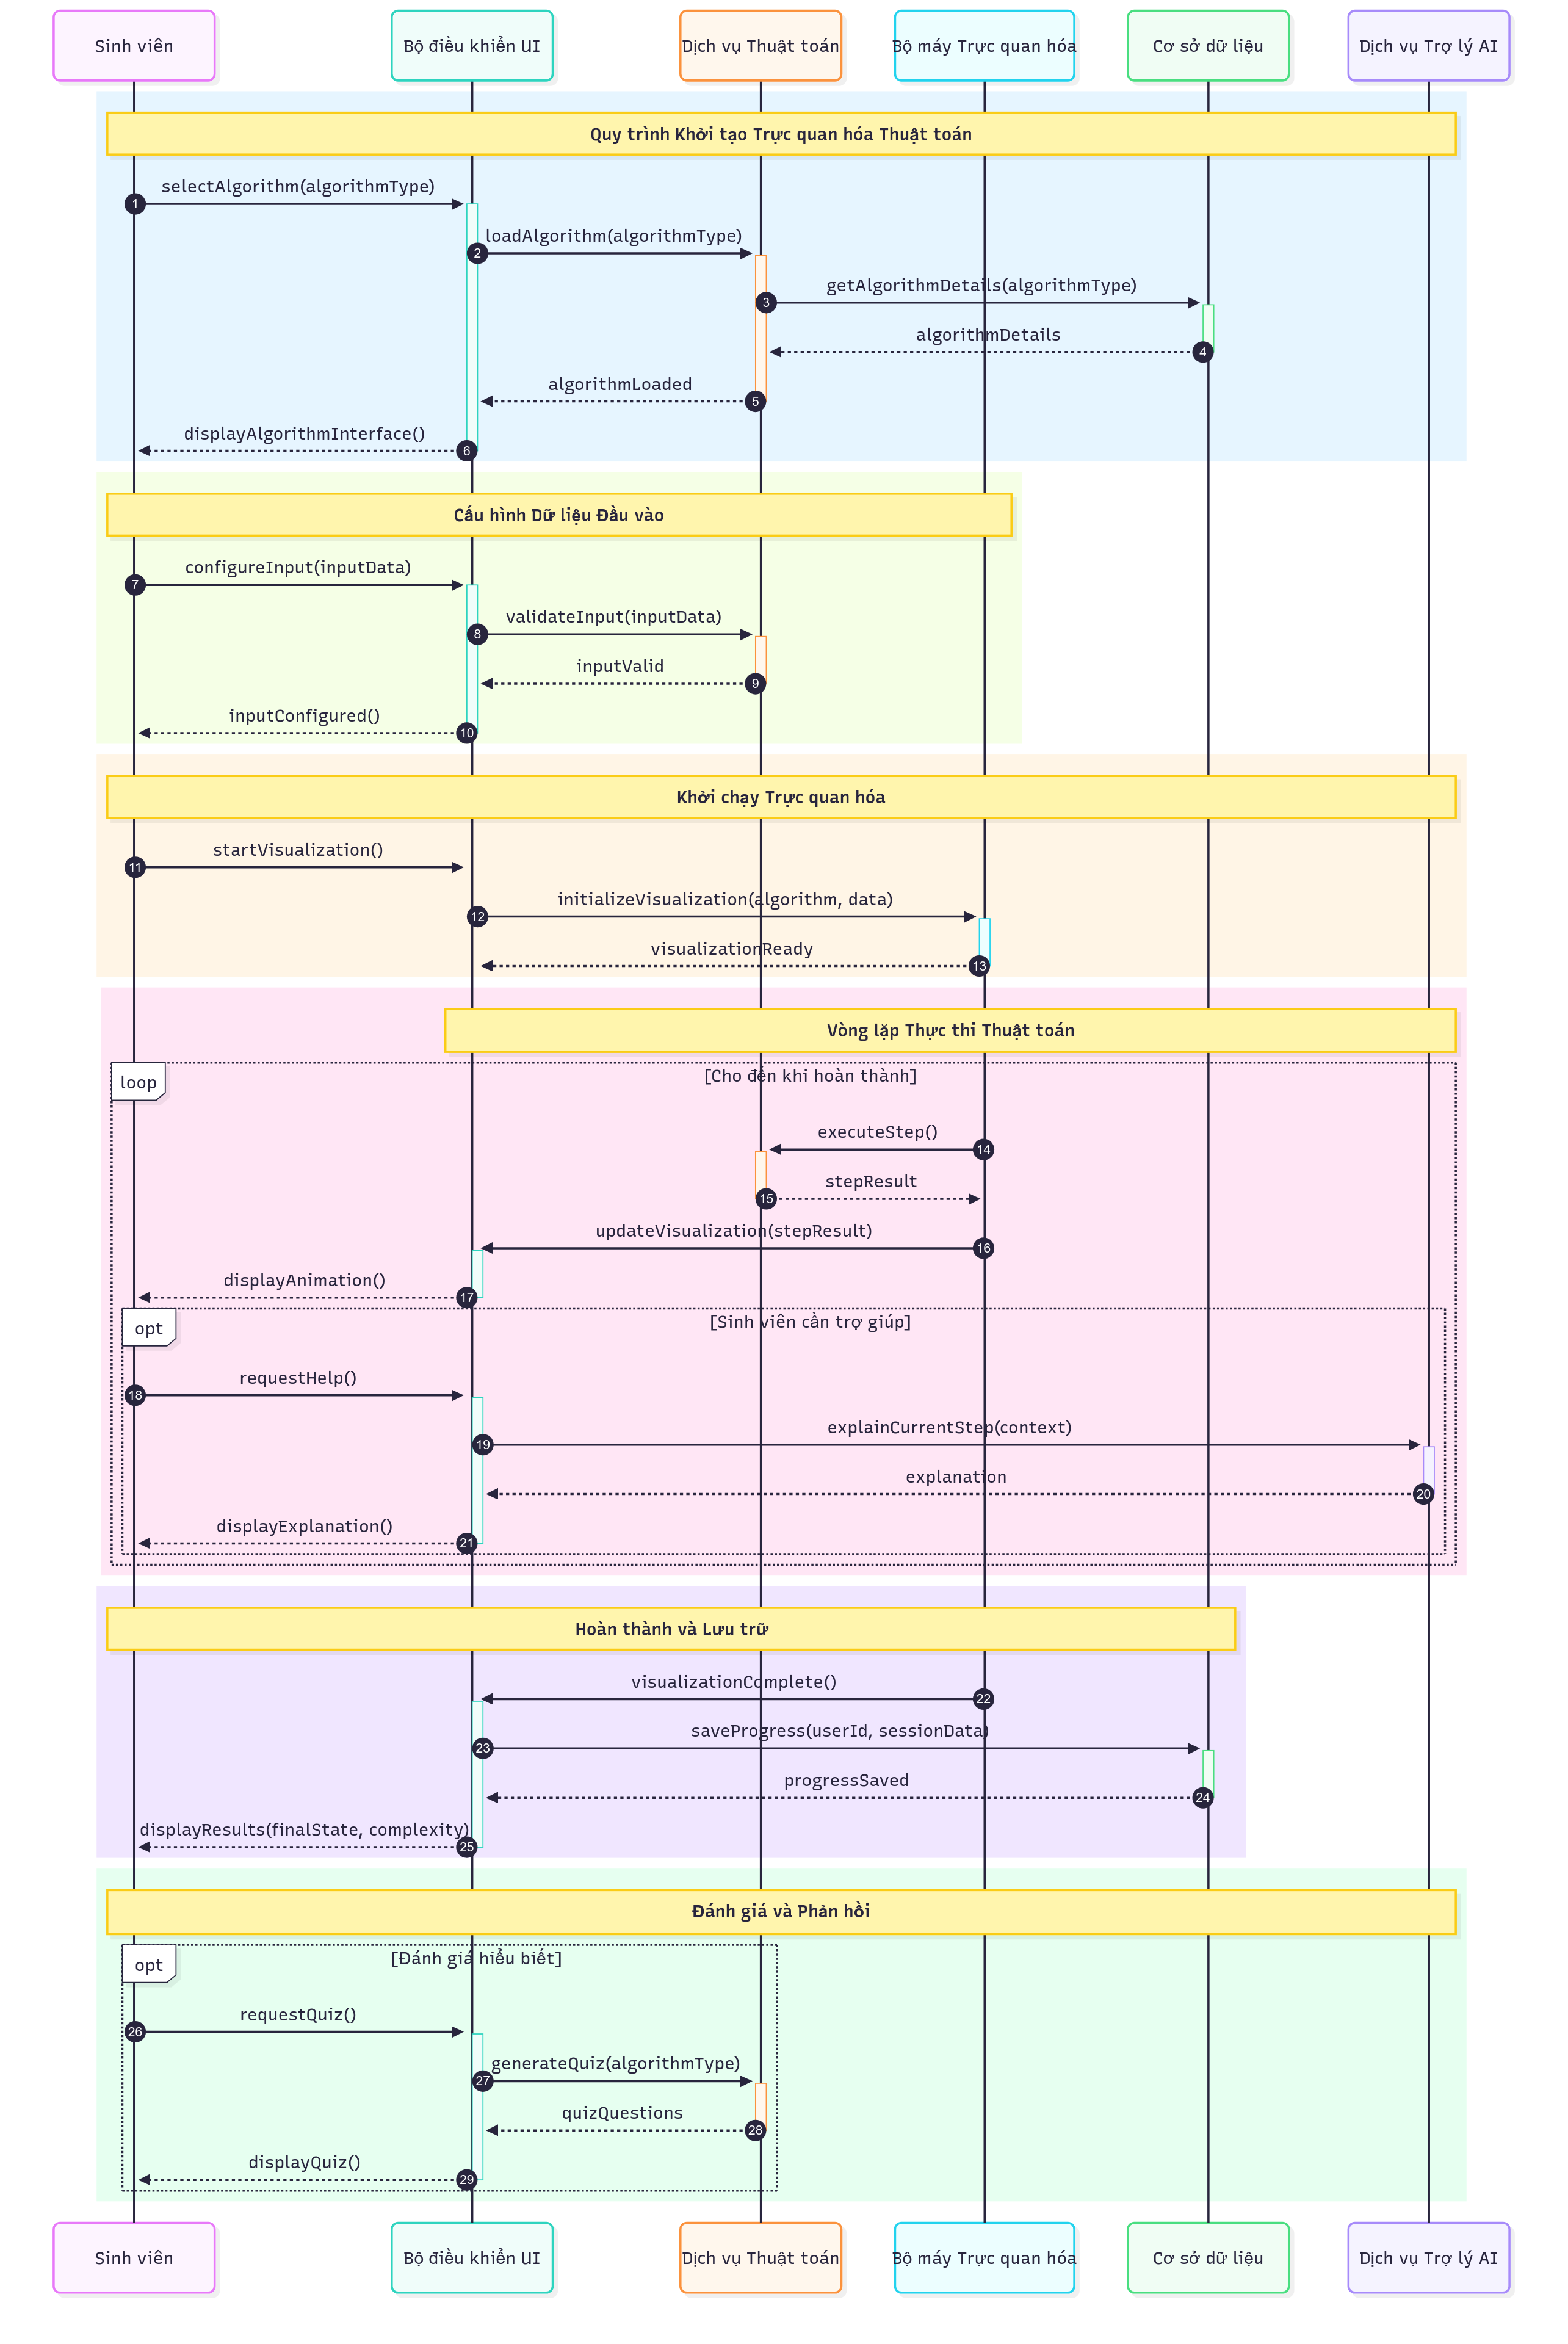
\includegraphics[width=0.95\textwidth]{images/sequence-algorithm-visualization.png}
\caption{Sequence Diagram - Quy trình Trực quan hóa Thuật toán}
\label{fig:sequence-algorithm-visualization}
\end{figure}

\textbf{Các giai đoạn chính:}
\begin{enumerate}
    \item \textbf{Khởi tạo}: Chọn thuật toán và tải cấu hình
    \item \textbf{Cấu hình}: Thiết lập dữ liệu đầu vào và tham số
    \item \textbf{Thực thi}: Chạy thuật toán theo từng bước với trực quan hóa
    \item \textbf{Tương tác}: Hỗ trợ AI khi cần thiết
    \item \textbf{Hoàn thành}: Lưu tiến độ và hiển thị kết quả
\end{enumerate}

\subsection{Sequence Diagram: Tương tác Trợ lý AI}
\label{subsec:ai-assistant-sequence}

Biểu đồ này chi tiết hóa cách thức hoạt động của hệ thống AI Assistant, từ khởi tạo phiên làm việc đến cung cấp khuyến nghị cá nhân hóa.

\begin{figure}[H]
\centering
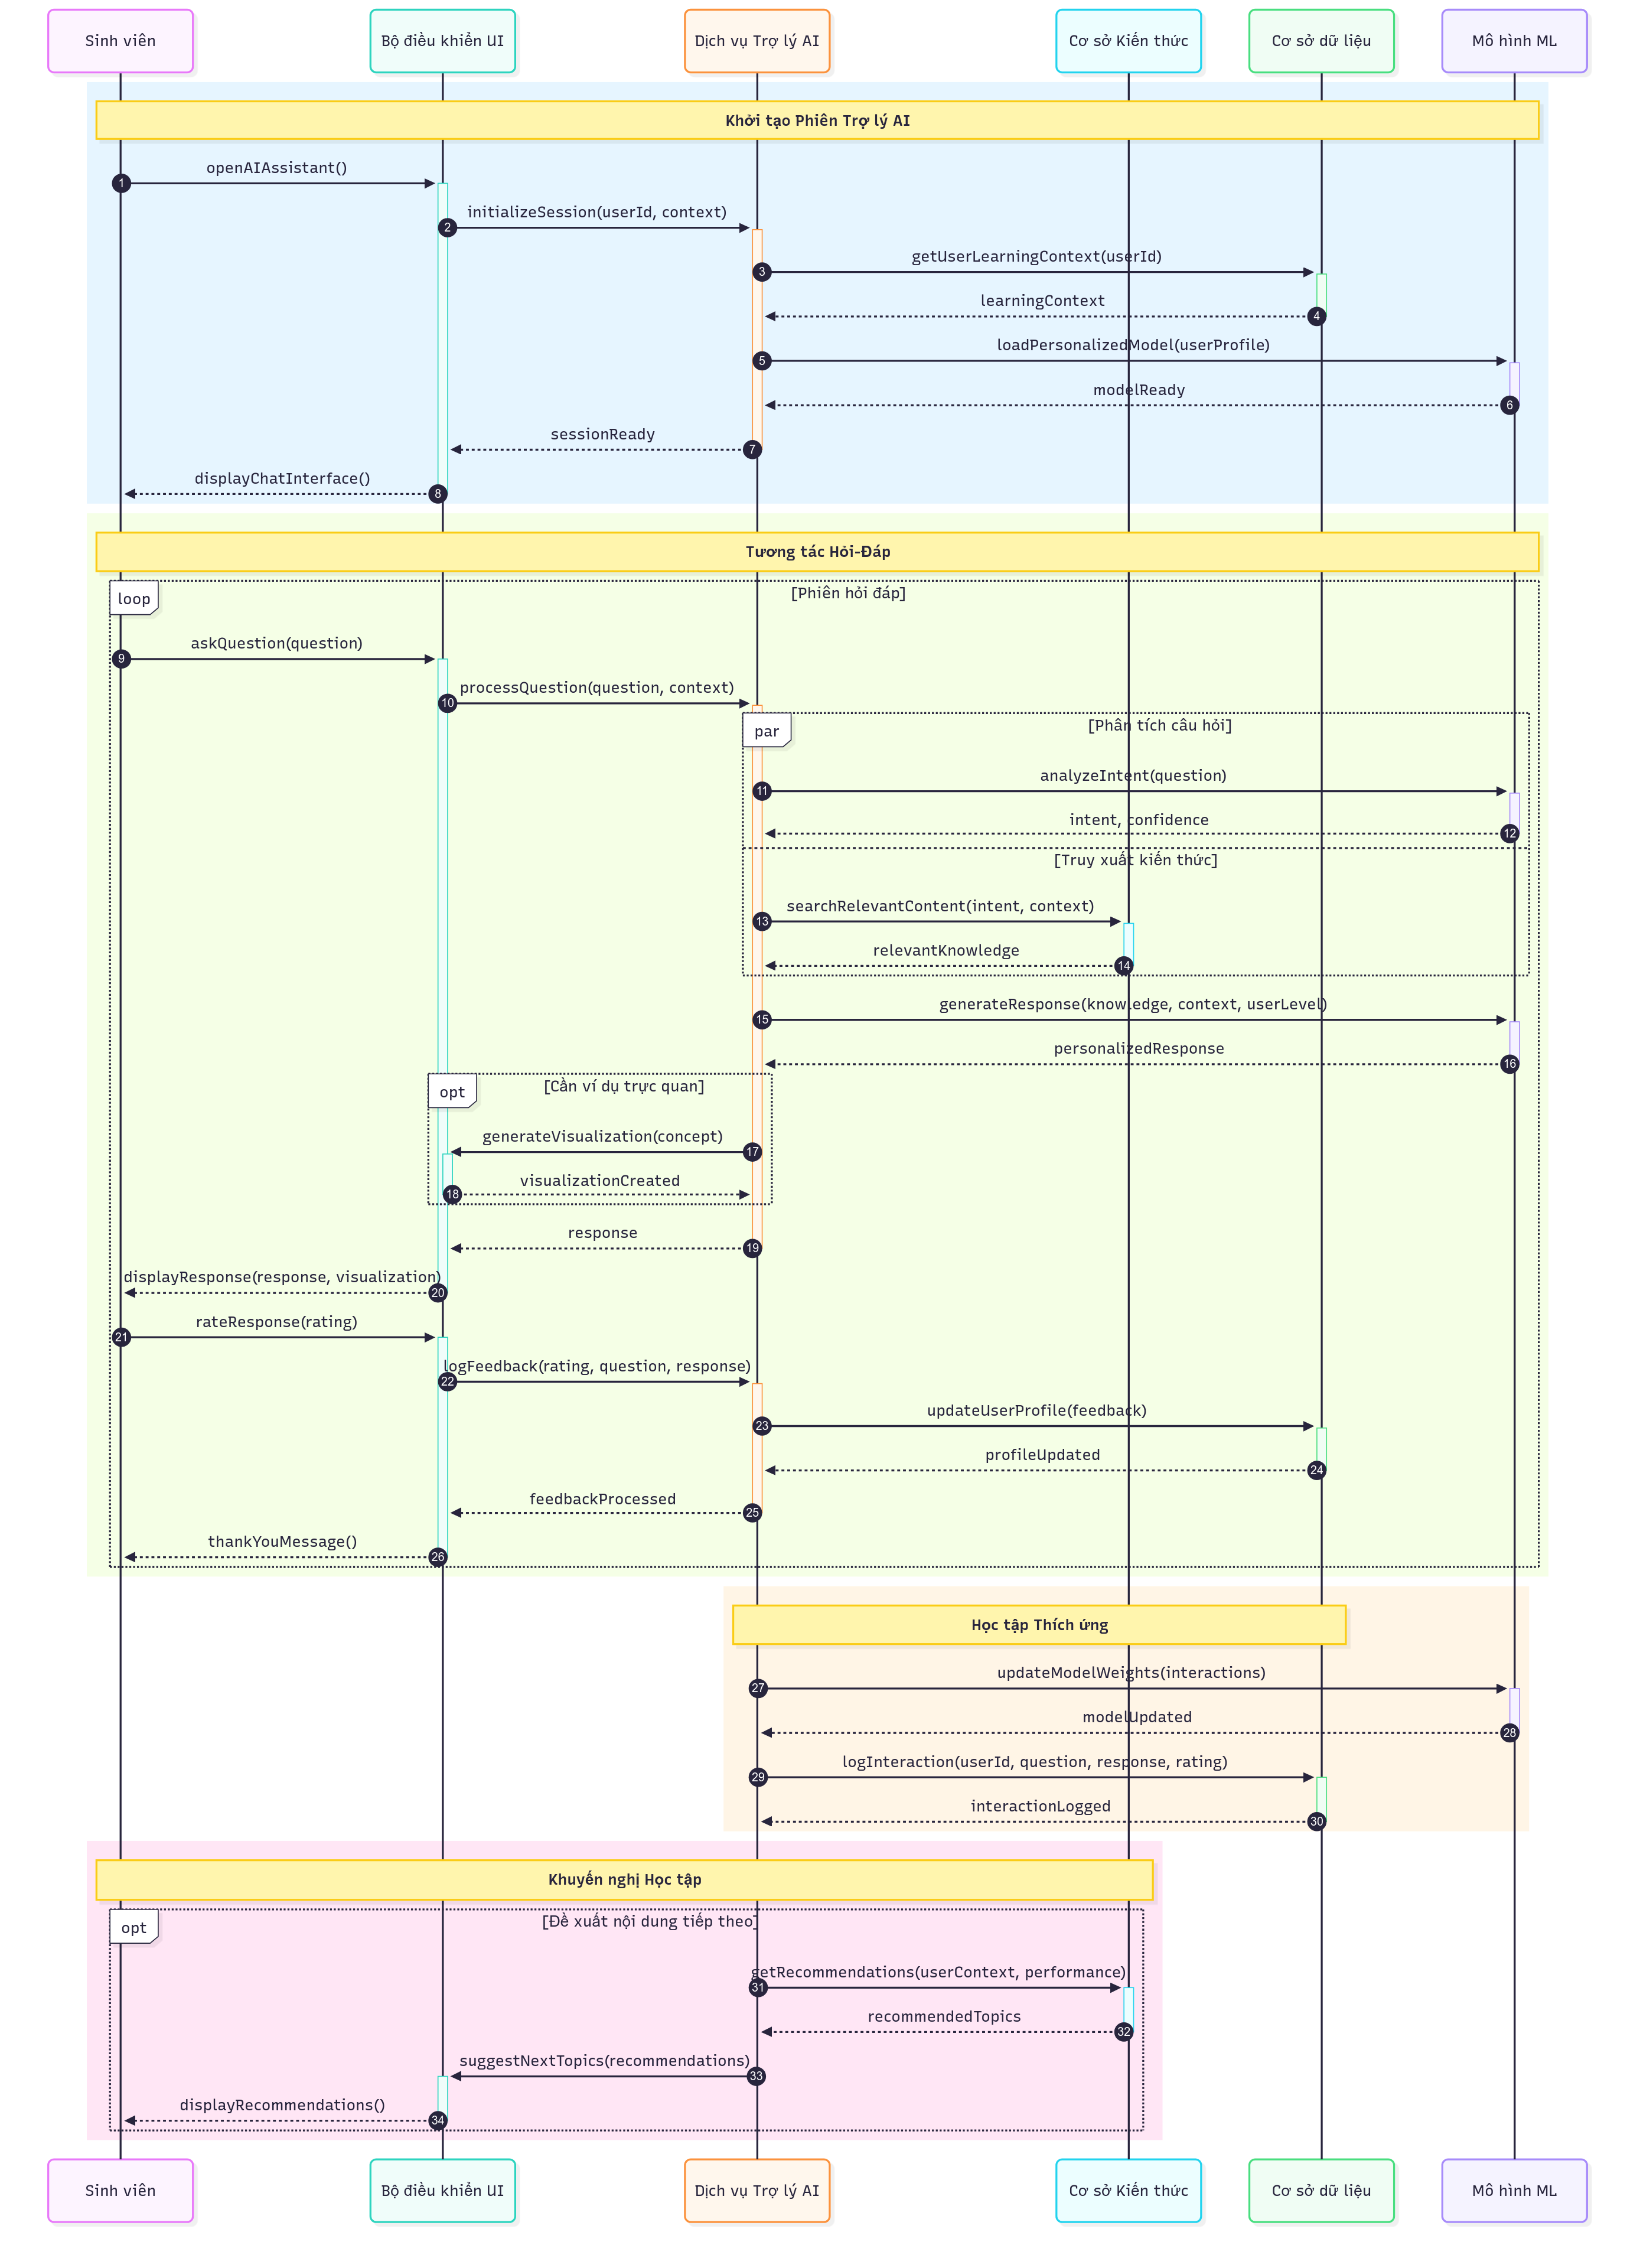
\includegraphics[width=0.95\textwidth]{images/sequence-ai-assistant.png}
\caption{Sequence Diagram - Tương tác Trợ lý AI}
\label{fig:sequence-ai-assistant}
\end{figure}

\textbf{Đặc điểm nổi bật:}
\begin{itemize}
    \item \textbf{Cá nhân hóa}: AI điều chỉnh phản hồi dựa trên profile người học
    \item \textbf{Xử lý song song}: Phân tích intent và truy xuất kiến thức đồng thời
    \item \textbf{Học thích ứng}: Cập nhật model dựa trên feedback của người dùng
    \item \textbf{Trực quan hóa tích hợp}: Tạo visualization để minh họa khái niệm
\end{itemize}

\subsection{Sequence Diagram: Hệ thống Đánh giá}
\label{subsec:assessment-sequence}

Mô tả quy trình đánh giá thích ứng với khả năng điều chỉnh độ khó theo thời gian thực.

\begin{figure}[H]
\centering
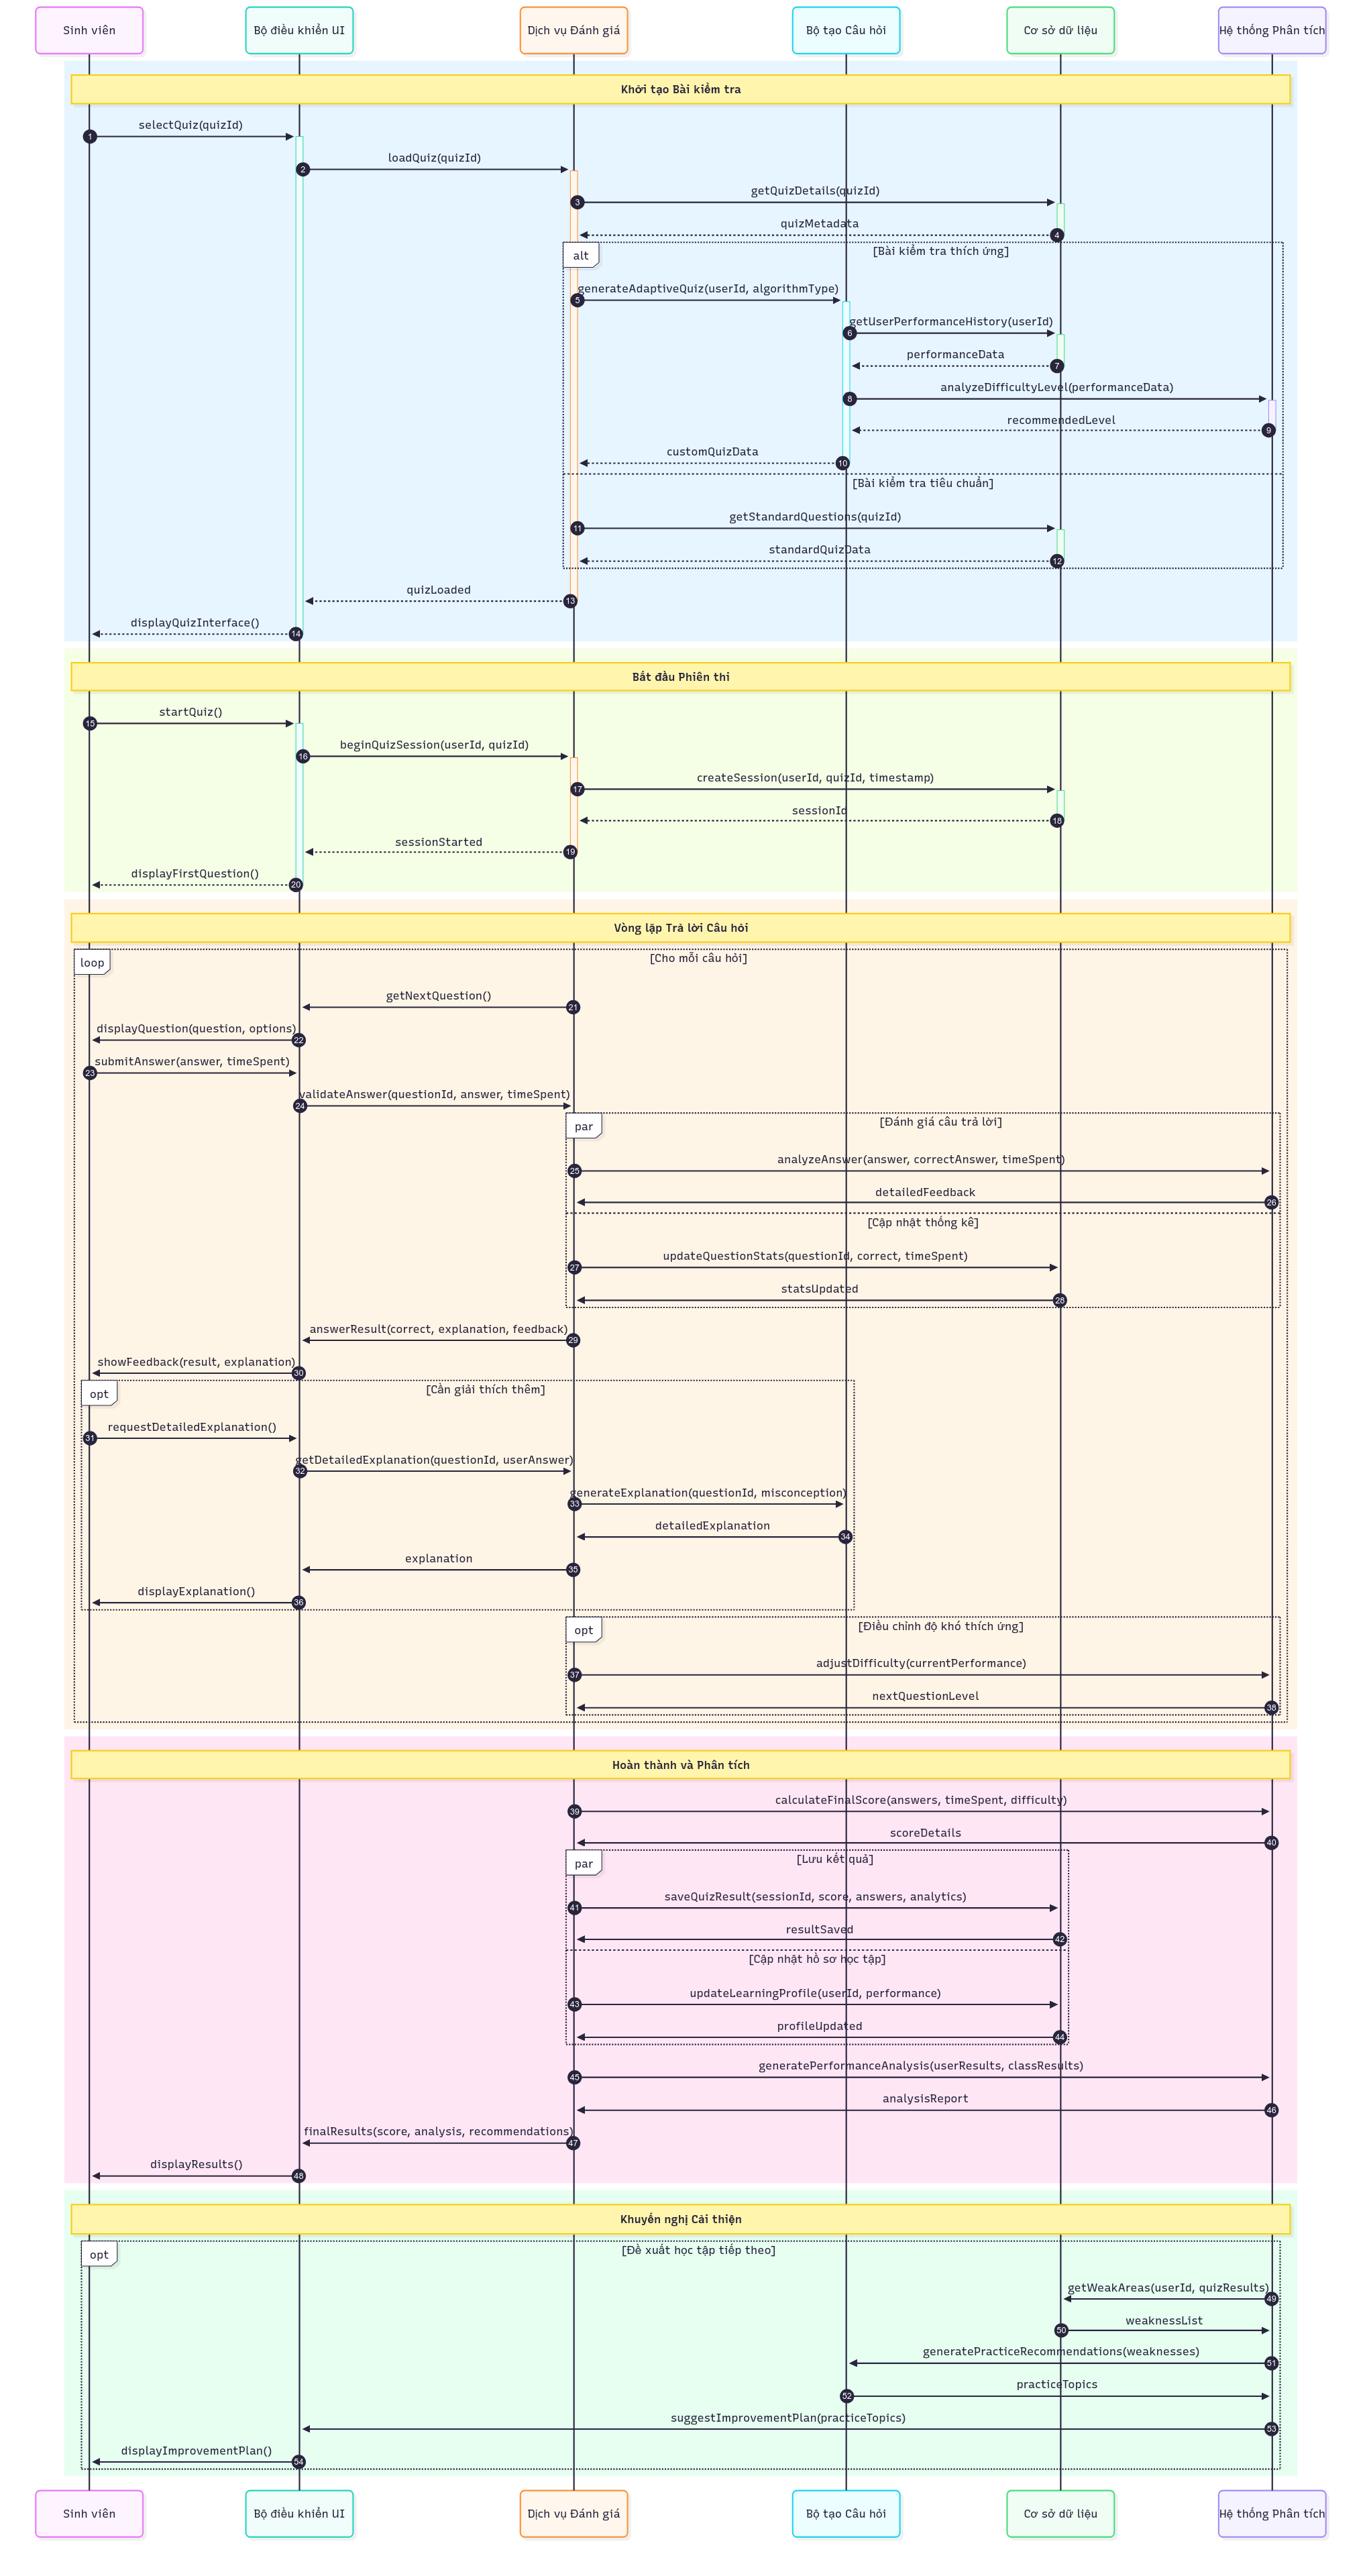
\includegraphics[width=0.95\textwidth]{images/sequence-assessment-system.png}
\caption{Sequence Diagram - Hệ thống Đánh giá}
\label{fig:sequence-assessment-system}
\end{figure}

\textbf{Tính năng tiên tiến:}
\begin{itemize}
    \item \textbf{Đánh giá thích ứng}: Điều chỉnh độ khó dựa trên hiệu suất hiện tại
    \item \textbf{Phân tích chi tiết}: Đánh giá sâu về thời gian và pattern trả lời
    \item \textbf{Feedback tức thì}: Giải thích chi tiết cho từng câu trả lời
    \item \textbf{Khuyến nghị cải thiện}: Đề xuất lộ trình học cụ thể
\end{itemize}

\subsection{Sequence Diagram: Tương tác Hệ thống Tổng thể}
\label{subsec:complete-system-sequence}

Biểu đồ tổng hợp mô tả luồng tương tác hoàn chỉnh từ đăng nhập đến hoàn thành phiên học.

\begin{figure}[H]
\centering
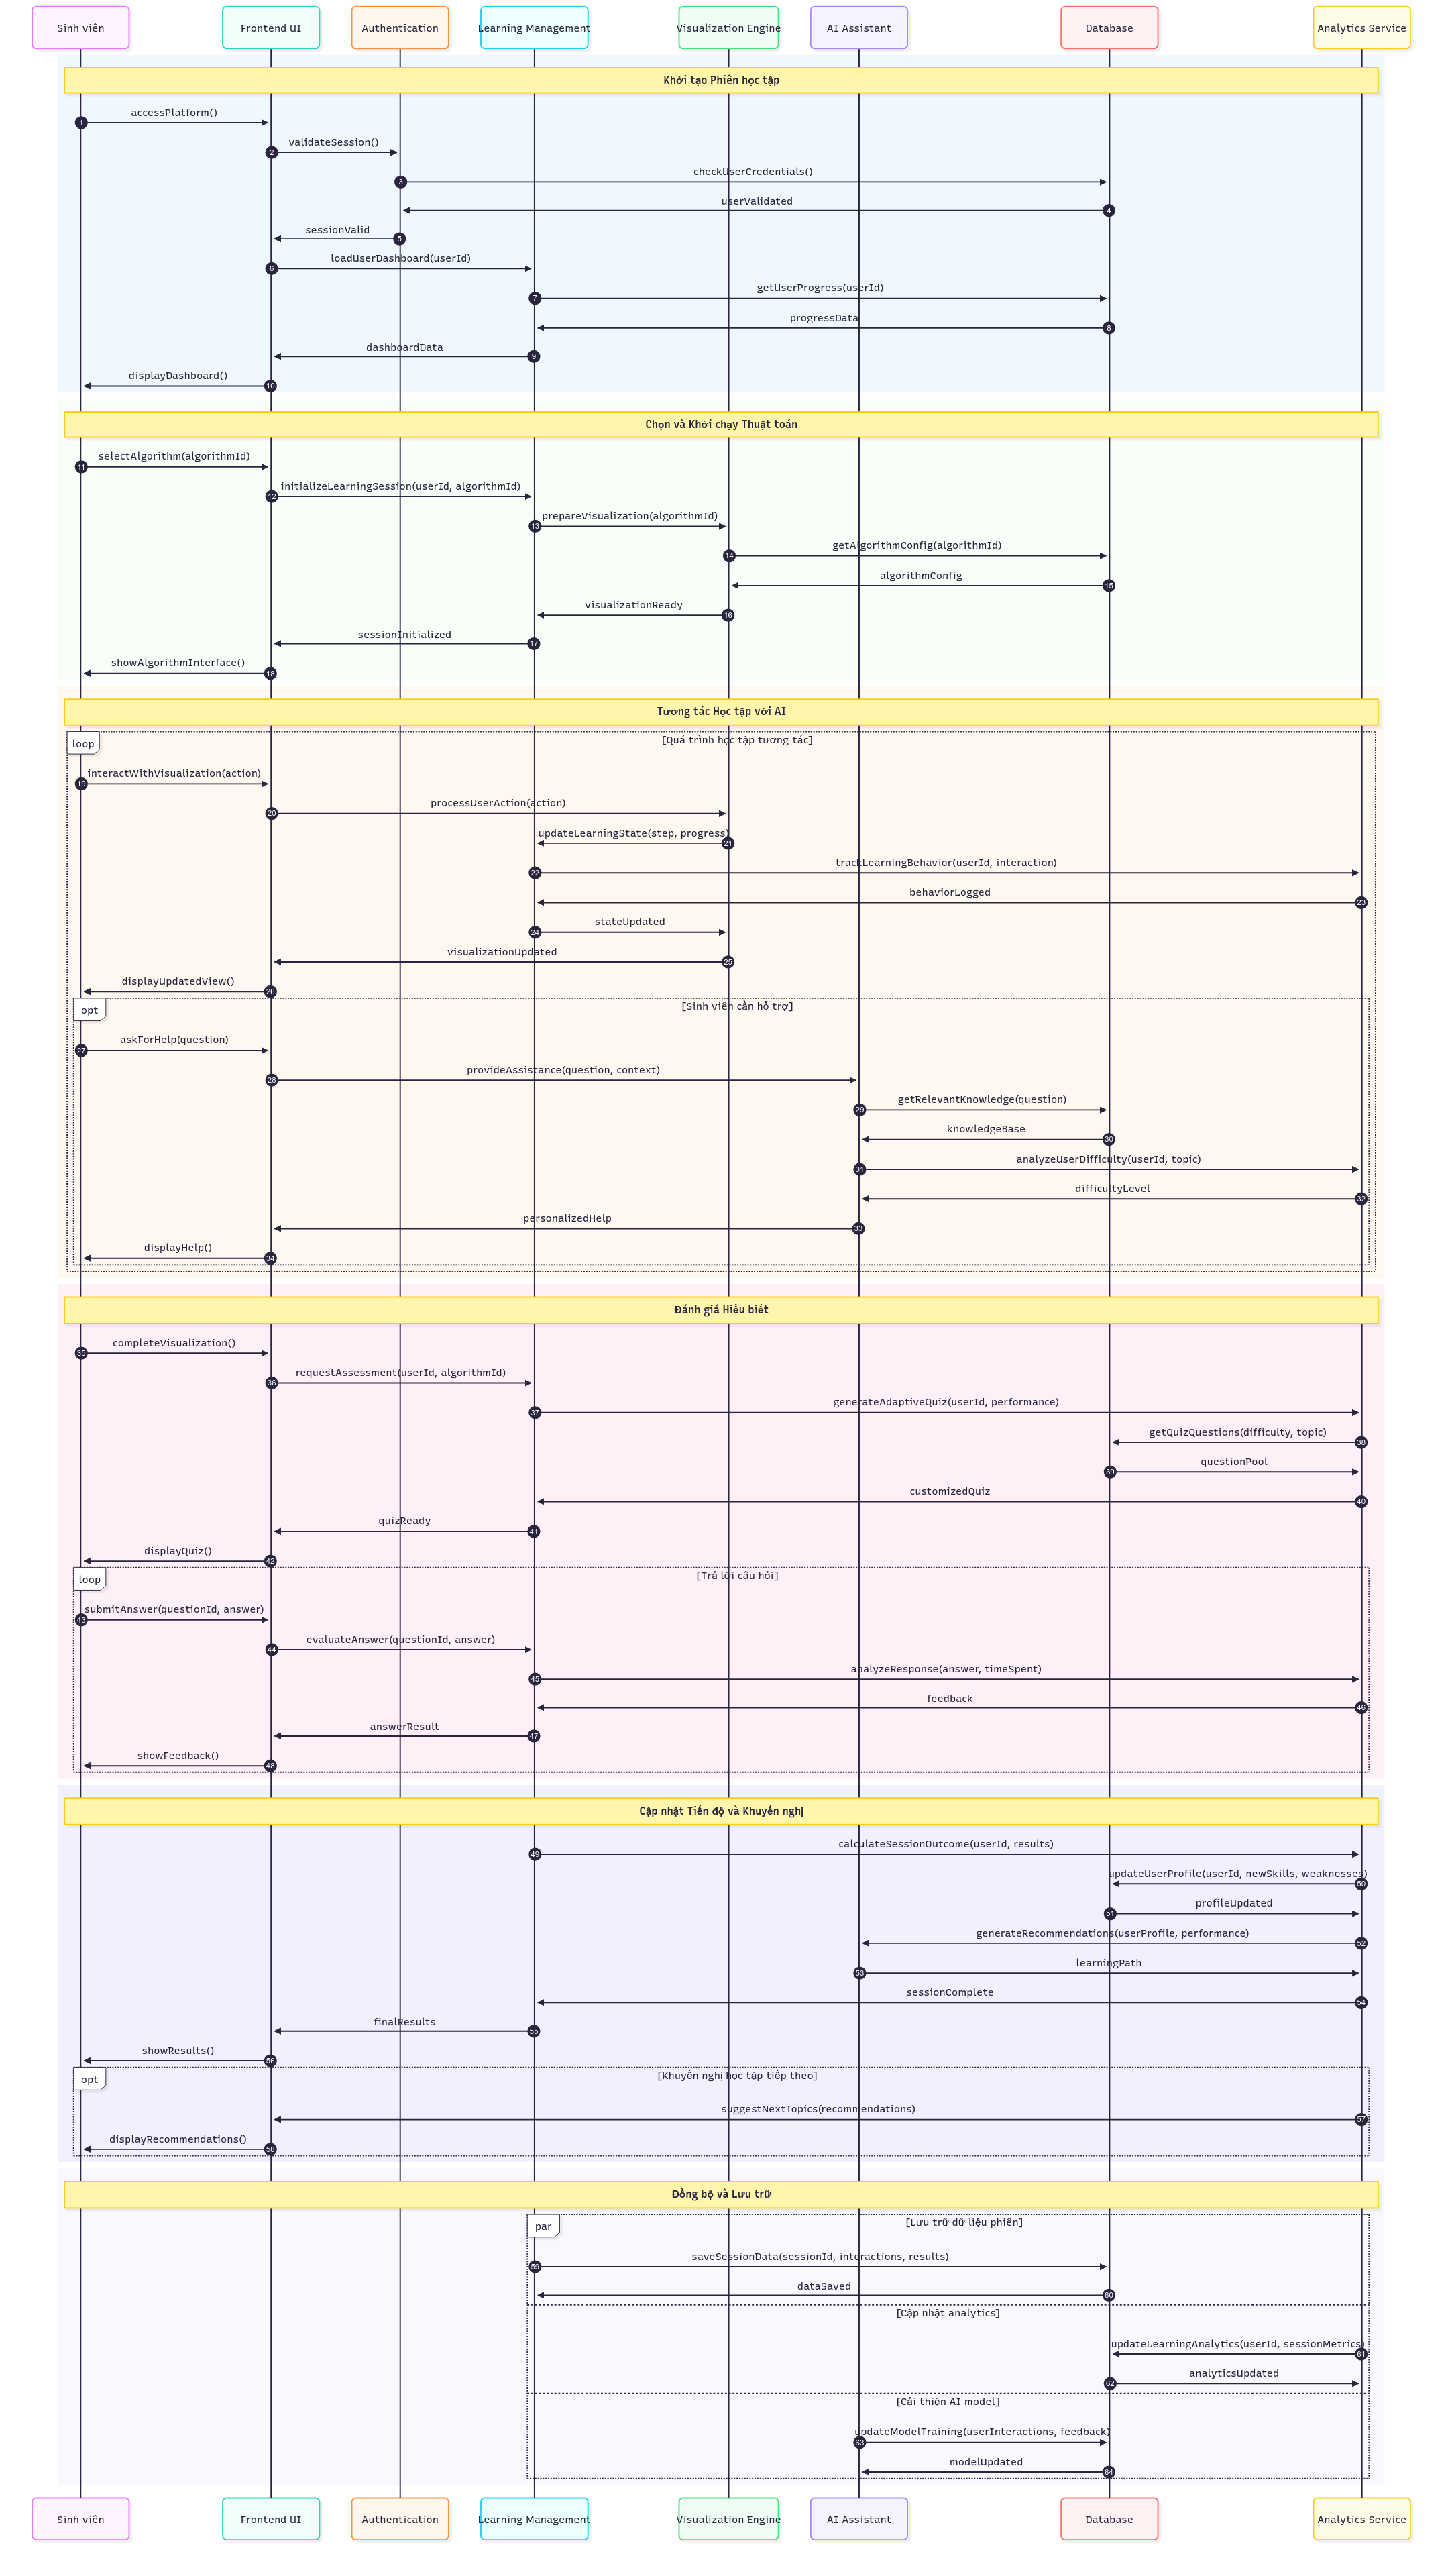
\includegraphics[width=0.95\textwidth]{images/sequence-complete-system.png}
\caption{Sequence Diagram - Hệ thống Hoàn chỉnh}
\label{fig:sequence-complete-system}
\end{figure}

\textbf{Kiến trúc tích hợp:}
\begin{itemize}
    \item \textbf{Authentication}: Quản lý phiên và bảo mật
    \item \textbf{Learning Management}: Điều phối toàn bộ quá trình học
    \item \textbf{Analytics Service}: Thu thập và phân tích dữ liệu học tập
    \item \textbf{Xử lý song song}: Tối ưu hóa hiệu suất hệ thống
\end{itemize}
\end{enumerate}

\subsection{Chuỗi Xử lý Lỗi}

\subsubsection{Chuỗi Lỗi Xác thực}
\begin{enumerate}
    \item \textbf{Sinh viên → Bộ điều khiển UI:} login(credentials)
    \item \textbf{Bộ điều khiển UI → Dịch vụ Xác thực:} validateCredentials(credentials)
    \item \textbf{Dịch vụ Xác thực → Cơ sở dữ liệu:} checkUserCredentials(credentials)
    \item \textbf{Cơ sở dữ liệu → Dịch vụ Xác thực:} userNotFound/invalidPassword
    \item \textbf{Dịch vụ Xác thực → Bộ điều khiển UI:} authenticationFailed(errorType)
    \item \textbf{Bộ điều khiển UI → Sinh viên:} displayErrorMessage(errorType)
    \item \textbf{Bộ điều khiển UI → Sinh viên:} requestCredentialsAgain()
\end{enumerate}

\subsubsection{Chuỗi Khôi phục Lỗi Hệ thống}
\begin{enumerate}
    \item \textbf{Dịch vụ bất kỳ:} systemError(errorDetails)
    \item \textbf{Bộ xử lý Lỗi:} logError(errorDetails)
    \item \textbf{Bộ xử lý Lỗi → Dịch vụ Giám sát:} reportError(errorDetails)
    \item \textbf{Bộ xử lý Lỗi → Bộ điều khiển UI:} notifyUser(genericErrorMessage)
    \item \textbf{Bộ điều khiển UI → Sinh viên:} displayErrorScreen(recoveryOptions)
    \item \textbf{Bộ xử lý Lỗi:} attemptRecovery()
    \item \textbf{Dịch vụ Dự phòng:} provideFallbackFunctionality()
\end{enumerate}

\section{Phân tích Kiến trúc Hệ thống}
\label{sec:system-architecture}

\subsection{Tổng quan Kiến trúc}
\label{subsec:architecture-overview}

Hệ thống DSA Visualizer được thiết kế theo mô hình kiến trúc 5 tầng để đảm bảo khả năng mở rộng, dễ bảo trì và tối ưu hóa hiệu suất.

\begin{center}
\textbf{[Biểu đồ Kiến trúc Hệ thống]}\\
\textit{Diagram: system-architecture.drawio}
\end{center}

\subsection{Chi tiết các Tầng}

\subsubsection{Tầng UI (Tầng Trình bày)}
\textbf{Công nghệ sử dụng:} Next.js 14, React 18, TypeScript, TailwindCSS

\textbf{Thành phần chính:}
\begin{itemize}
    \item \textbf{Trình trực quan hóa Tương tác:} Hoạt hình thuật toán dựa trên Canvas
    \item \textbf{Bảng điều khiển:} Điều khiển tốc độ, điều hướng từng bước
    \item \textbf{Giao diện Bảng điều khiển:} Theo dõi tiến độ và thống kê người dùng
    \item \textbf{Giao diện Trò chuyện AI:} Trò chuyện thời gian thực với Trợ lý AI
    \item \textbf{Giao diện Đánh giá:} Bài kiểm tra và bài tập thực hành
\end{itemize}

\textbf{Mẫu Thiết kế:}
\begin{itemize}
    \item Kiến trúc dựa trên thành phần
    \item Quản lý trạng thái với Context API
    \item Hook tùy chỉnh cho logic có thể tái sử dụng
    \item Mẫu thiết kế đáp ứng
\end{itemize}

\subsubsection{Tầng Bộ máy Trực quan hóa}
\textbf{Công nghệ sử dụng:} D3.js, Canvas API, WebGL

\textbf{Thành phần Cốt lõi:}
\begin{itemize}
    \item \textbf{Bộ điều khiển Hoạt hình:} Quản lý dòng thời gian và trạng thái hoạt hình
    \item \textbf{Bộ máy Hiển thị:} Hiển thị trực quan hóa hiệu suất cao
    \item \textbf{Bộ xử lý Tương tác:} Xử lý đầu vào người dùng cho trực quan hóa
    \item \textbf{Quản lý Trạng thái:} Theo dõi trạng thái thuật toán và lịch sử
\end{itemize}

\textbf{Các loại Trực quan hóa:}
\begin{itemize}
    \item Trực quan hóa Mảng/Danh sách với mã hóa màu
    \item Cấu trúc Cây với các nút tương tác
    \item Trực quan hóa Đồ thị với hoạt hình cạnh
    \item Khung nhìn So sánh cho nhiều thuật toán
\end{itemize}

\subsubsection{Tầng Dịch vụ Backend}
\textbf{Công nghệ sử dụng:} Node.js, Express.js, TypeScript

\textbf{Kiến trúc Microservices:}
\begin{itemize}
    \item \textbf{Dịch vụ Thuật toán:} Thực thi thuật toán và tạo bước
    \item \textbf{Dịch vụ Người dùng:} Xác thực, quản lý hồ sơ
    \item \textbf{Dịch vụ Học tập:} Theo dõi tiến độ, quản lý phiên
    \item \textbf{Dịch vụ Đánh giá:} Tạo bài kiểm tra, hệ thống chấm điểm
    \item \textbf{Dịch vụ AI:} Xử lý ngôn ngữ tự nhiên, truy xuất kiến thức
    \item \textbf{Dịch vụ Phân tích:} Theo dõi hành vi người dùng, chỉ số hiệu suất
\end{itemize}

\textbf{Thiết kế API:}
\begin{itemize}
    \item API RESTful với tài liệu OpenAPI
    \item Điểm cuối GraphQL cho truy vấn dữ liệu phức tạp
    \item Kết nối WebSocket cho tính năng thời gian thực
    \item Giới hạn tốc độ và middleware bảo mật
\end{itemize}

\subsubsection{Tầng Quản lý Dữ liệu}
\textbf{Công nghệ sử dụng:} MongoDB, Redis, PostgreSQL

\textbf{Chiến lược Cơ sở dữ liệu:}
\begin{itemize}
    \item \textbf{MongoDB:} Hồ sơ người dùng, phiên học tập, siêu dữ liệu thuật toán
    \item \textbf{PostgreSQL:} Dữ liệu có cấu trúc, phân tích, báo cáo
    \item \textbf{Redis:} Lưu trữ phiên, dữ liệu thời gian thực, bảng xếp hạng
\end{itemize}

\textbf{Mô hình Dữ liệu:}
\begin{itemize}
    \item Thực thể Người dùng và Hồ sơ với ánh xạ mối quan hệ
    \item Siêu dữ liệu thuật toán với phân tích độ phức tạp
    \item Tiến độ học tập với theo dõi chi tiết
    \item Kết quả đánh giá với phân tích thống kê
\end{itemize}

\subsubsection{Tầng Hạ tầng}
\textbf{Chiến lược Triển khai:} Container Docker, điều phối Kubernetes

\textbf{Dịch vụ Đám mây:}
\begin{itemize}
    \item \textbf{Tính toán:} Máy chủ web tự động mở rộng
    \item \textbf{Lưu trữ:} Lưu trữ tệp phân tán cho tài sản
    \item \textbf{CDN:} Mạng phân phối nội dung toàn cầu
    \item \textbf{Giám sát:} Giám sát hiệu suất ứng dụng
\end{itemize}

\textbf{Biện pháp Bảo mật:}
\begin{itemize}
    \item Xác thực dựa trên JWT với token làm mới
    \item Thực thi HTTPS với chứng chỉ SSL
    \item Xác thực đầu vào và ngăn chặn SQL injection
    \item Cấu hình Chia sẻ Tài nguyên Có nguồn gốc (CORS)
\end{itemize}

\subsection{Mẫu Tích hợp}

\subsubsection{Kiến trúc Hướng sự kiện}
\begin{itemize}
    \item Sự kiện hành động người dùng kích hoạt cập nhật trực quan hóa
    \item Sự kiện tiến độ cập nhật phân tích học tập
    \item Sự kiện thành tích kích hoạt hệ thống thông báo
    \item Sự kiện lỗi kích hoạt giám sát và cảnh báo
\end{itemize}

\subsubsection{Chiến lược Bộ nhớ đệm}
\begin{itemize}
    \item Bộ nhớ đệm trình duyệt cho tài sản tĩnh
    \item Bộ nhớ đệm Redis cho dữ liệu được truy cập thường xuyên
    \item Bộ nhớ đệm CDN cho hiệu suất toàn cầu
    \item Bộ nhớ đệm cấp ứng dụng cho kết quả tính toán
\end{itemize}

\section{Nguyên tắc Thiết kế và Thực hành Tốt nhất}
\label{sec:design-principles}

\subsection{Triển khai Nguyên tắc SOLID}

\subsubsection{Nguyên tắc Trách nhiệm Duy nhất}
Mỗi lớp và thành phần có một trách nhiệm duy nhất:
\begin{itemize}
    \item VisualizationRenderer chỉ xử lý logic hiển thị
    \item AlgorithmExecutor chỉ xử lý thực thi thuật toán
    \item UserManager chỉ xử lý các hoạt động liên quan đến người dùng
\end{itemize}

\subsubsection{Nguyên tắc Mở/Đóng}
Hệ thống được thiết kế để mở rộng chức năng mà không cần sửa đổi:
\begin{itemize}
    \item Kiến trúc plugin cho các loại thuật toán mới
    \item Hệ thống mở rộng cho trực quan hóa tùy chỉnh
    \item Khung đánh giá có thể cấu hình
\end{itemize}

\subsubsection{Nguyên tắc Thay thế Liskov}
Các lớp trừu tượng và giao diện đảm bảo khả năng thay thế:
\begin{itemize}
    \item Giao diện Algorithm có thể được triển khai bởi bất kỳ loại thuật toán nào
    \item Giao diện Visualizer hỗ trợ nhiều chiến lược hiển thị
    \item Giao diện Assessment phù hợp với các loại bài kiểm tra khác nhau
\end{itemize}

\subsection{Tối ưu hóa Hiệu suất}

\subsubsection{Tối ưu hóa Frontend}
\begin{itemize}
    \item Chia tách mã và tải lười cho các thành phần
    \item Ghi nhớ cho các phép tính tốn kém
    \item Cuộn ảo cho tập dữ liệu lớn
    \item Debouncing cho xử lý đầu vào người dùng
\end{itemize}

\subsubsection{Tối ưu hóa Backend}
\begin{itemize}
    \item Tối ưu hóa truy vấn cơ sở dữ liệu với chỉ mục phù hợp
    \item Gộp kết nối cho kết nối cơ sở dữ liệu
    \item Xử lý bất đồng bộ cho các tác vụ tốn thời gian
    \item Cân bằng tải cho tính khả dụng cao
\end{itemize}

\subsection{Khả năng Tiếp cận và Khả năng Sử dụng}

\subsubsection{Tính năng Khả năng Tiếp cận}
\begin{itemize}
    \item Tuân thủ WCAG 2.1 cho tiêu chuẩn khả năng tiếp cận
    \item Hỗ trợ điều hướng bằng bàn phím
    \item Tương thích với trình đọc màn hình
    \item Chế độ tương phản cao cho khiếm thị
\end{itemize}

\subsubsection{Tính năng Khả năng Sử dụng}
\begin{itemize}
    \item Thiết kế giao diện người dùng trực quan
    \item Tiết lộ dần dần các tính năng phức tạp
    \item Trợ giúp ngữ cảnh và chú giải công cụ
    \item Thiết kế đáp ứng cho nhiều thiết bị
\end{itemize}

\section{Kết luận Chương 3}
\label{sec:chapter3-conclusion}

Chương 3 đã phân tích chi tiết hệ thống DSA Visualizer từ góc độ kiến trúc kỹ thuật và thiết kế. Các điểm chính bao gồm:

\subsection{Phân tích Use Case}
Đã định nghĩa và mô tả chi tiết các use case chính của hệ thống, bao gồm học tập thuật toán, thực hành tương tác, và tư vấn trợ lý AI. Mỗi use case được tài liệu hóa với định dạng bảng chi tiết theo chuẩn học thuật.

\subsection{Phân tích Biểu đồ UML}
\begin{itemize}
    \item \textbf{Biểu đồ Lớp:} Thiết kế OOP với các mẫu thiết kế phù hợp
    \item \textbf{Biểu đồ Hoạt động:} Mô tả chi tiết quy trình hoạt động và luồng quyết định
    \item \textbf{Biểu đồ Tuần tự:} Phân tích tương tác giữa đối tượng theo dòng thời gian
\end{itemize}

\subsection{Kiến trúc Hệ thống}
Thiết kế kiến trúc 5 tầng đảm bảo:
\begin{itemize}
    \item Khả năng mở rộng cho việc mở rộng trong tương lai
    \item Khả năng bảo trì với thiết kế mô-đun
    \item Tối ưu hóa hiệu suất với chiến lược bộ nhớ đệm
    \item Bảo mật với các biện pháp bảo vệ toàn diện
\end{itemize}

\subsection{Xuất sắc Kỹ thuật}
Áp dụng nguyên tắc SOLID, mẫu thiết kế, và thực hành tốt nhất để tạo ra một hệ thống mạnh mẽ và chuyên nghiệp.

Tiếp theo, Chương 4 sẽ tập trung vào chi tiết triển khai và đặc tả kỹ thuật của từng thành phần.

\include{chapters/4-system-design}
\include{chapters/5-implementation}
\include{chapters/6-testing-evaluation}
\include{chapters/7-conclusion}

\nocite{*}
\addcontentsline{toc}{chapter}{References}
\printbibliography
\include{chapters/appendix}
\end{document}
\end{enumerate}

\subsection{Đối tượng sử dụng}

\begin{table}[H]
\centering
\caption{Phân loại người dùng hệ thống}
\begin{tabular}{|l|p{10cm}|}
\hline
\textbf{Nhóm người dùng} & \textbf{Mô tả và nhu cầu} \\
\hline
\textbf{Sinh viên} & Học tập các thuật toán cơ bản, thực hành coding, tham gia cộng đồng \\
\hline
\textbf{Giảng viên} & Sử dụng làm công cụ giảng dạy, tạo nội dung học tập, quản lý lớp học \\
\hline
\textbf{Lập trình viên} & Ôn tập thuật toán cho phỏng vấn, nghiên cứu thuật toán mới \\
\hline
\textbf{Người tự học} & Tìm hiểu thuật toán một cách tự động, có AI hỗ trợ \\
\hline
\textbf{Admin} & Quản lý hệ thống, theo dõi usage, xử lý feedback \\
\hline
\end{tabular}
\end{table}

\section{Phân tích yêu cầu}

\subsection{Yêu cầu chức năng}

\subsubsection{Hệ thống xác thực và phân quyền}
\begin{itemize}
    \item \textbf{RF-01}: Đăng ký/đăng nhập với email, Google, GitHub
    \item \textbf{RF-02}: Hệ thống phân quyền 4 cấp (Guest, User, Teacher, Admin)
    \item \textbf{RF-03}: Quản lý profile và theo dõi tiến độ học tập
    \item \textbf{RF-04}: Password reset và email verification
\end{itemize}

\subsubsection{Visualizer thuật toán}
\begin{itemize}
    \item \textbf{RF-05}: Trực quan hóa sorting algorithms (Quick, Merge, Heap, Radix, etc.)
    \item \textbf{RF-06}: Visualizer cho data structures (Binary Tree, AVL, Hash Table, etc.)
    \item \textbf{RF-07}: Graph algorithms (Dijkstra, BFS, DFS, MST)
    \item \textbf{RF-08}: Dynamic Programming và Pathfinding visualizations
    \item \textbf{RF-09}: Điều khiển tốc độ animation và step-by-step execution
    \item \textbf{RF-10}: Multiple view modes và theme options
\end{itemize}

\subsubsection{AI Learning Assistant}
\begin{itemize}
    \item \textbf{RF-11}: Code analysis và suggestions cho 6 ngôn ngữ
    \item \textbf{RF-12}: Interactive explanations và step-by-step guidance
    \item \textbf{RF-13}: Algorithm optimization recommendations
    \item \textbf{RF-14}: Real-time code feedback và error detection
\end{itemize}

\subsubsection{Community Features}
\begin{itemize}
    \item \textbf{RF-15}: Discussion forums với threading và moderation
    \item \textbf{RF-16}: Q\&A system kiểu Stack Overflow
    \item \textbf{RF-17}: Rating và voting system
    \item \textbf{RF-18}: Real-time notifications và comments
\end{itemize}

\subsubsection{Admin Dashboard}
\begin{itemize}
    \item \textbf{RF-19}: User management và role assignment
    \item \textbf{RF-20}: Analytics và usage tracking
    \item \textbf{RF-21}: Feedback management và response system
    \item \textbf{RF-22}: System monitoring và performance metrics
\end{itemize}

\subsection{Yêu cầu phi chức năng}

\subsubsection{Hiệu năng}
\begin{itemize}
    \item \textbf{NFR-01}: Page load time < 2 giây
    \item \textbf{NFR-02}: Animation frame rate >= 60 FPS
    \item \textbf{NFR-03}: API response time < 500ms
    \item \textbf{NFR-04}: Support đồng thời 1000+ concurrent users
\end{itemize}

\subsubsection{Khả năng sử dụng}
\begin{itemize}
    \item \textbf{NFR-05}: Responsive design cho mobile, tablet, desktop
    \item \textbf{NFR-06}: Accessibility theo chuẩn WCAG 2.1 AA
    \item \textbf{NFR-07}: Multi-language support (Vietnamese, English)
    \item \textbf{NFR-08}: Dark/Light mode với system preference detection
\end{itemize}

\subsubsection{Bảo mật}
\begin{itemize}
    \item \textbf{NFR-09}: HTTPS encryption cho tất cả communications
    \item \textbf{NFR-10}: JWT token-based authentication
    \item \textbf{NFR-11}: Input sanitization và SQL injection prevention
    \item \textbf{NFR-12}: Rate limiting cho API endpoints
\end{itemize}

\subsubsection{Khả năng mở rộng}
\begin{itemize}
    \item \textbf{NFR-13}: Modular architecture cho phép add algorithms mới
    \item \textbf{NFR-14}: Database scalability với connection pooling
    \item \textbf{NFR-15}: Serverless deployment trên Vercel
    \item \textbf{NFR-16}: CDN integration cho static assets
\end{itemize}

\section{Thiết kế hệ thống}

\subsection{Kiến trúc tổng quan}

DSA Visualizer Platform được xây dựng theo kiến trúc phân tầng modular với các thành phần được tách biệt rõ ràng:

\begin{figure}[H]
\centering
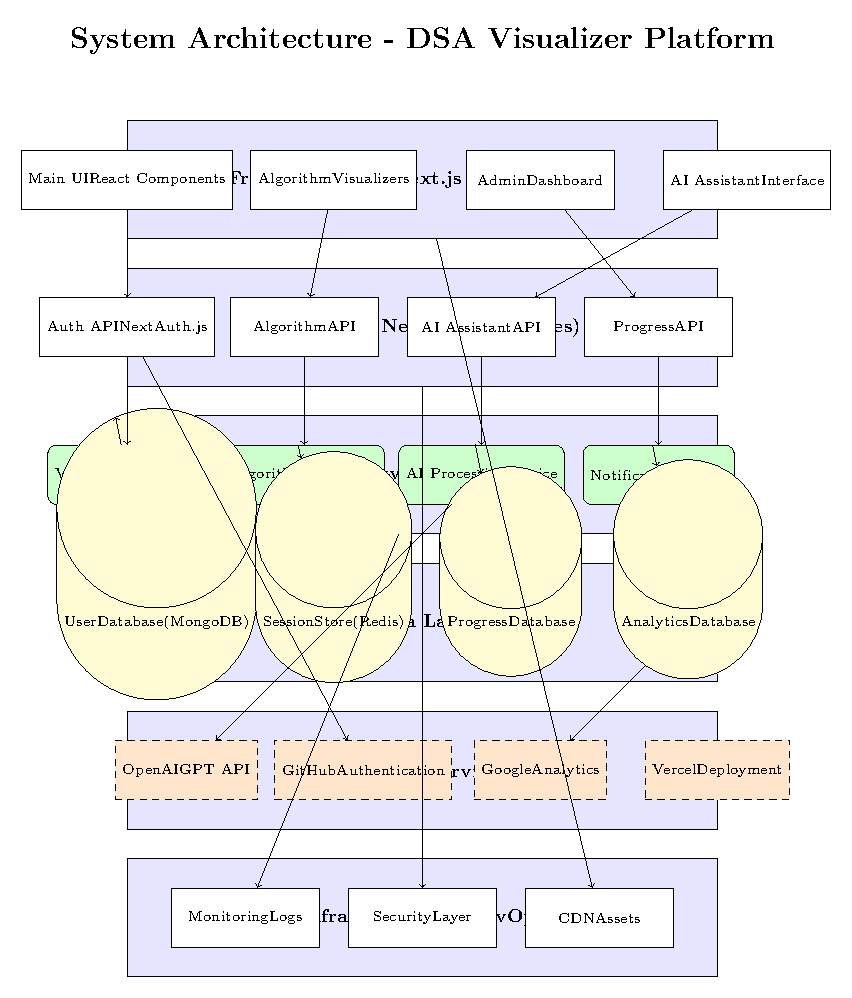
\includegraphics[width=0.9\textwidth]{diagrams/system_architecture.pdf}
\caption{Kiến trúc tổng thể hệ thống DSA Visualizer}
\label{fig:system_architecture}
\end{figure}

\subsubsection{Presentation Layer (Frontend)}
\begin{itemize}
    \item \textbf{Next.js 15 App Router}: Framework chính với server-side rendering
    \item \textbf{React 19}: UI library với concurrent features và hooks mới
    \item \textbf{TypeScript}: Type safety và developer experience
    \item \textbf{Tailwind CSS + shadcn/ui}: Modern styling với component library
    \item \textbf{Framer Motion}: Animation library cho smooth transitions
\end{itemize}

\subsubsection{Business Logic Layer}
\begin{itemize}
    \item \textbf{Algorithm Engines}: Core logic cho 24+ visualization algorithms
    \item \textbf{AI Integration}: OpenAI GPT và Google Gemini APIs
    \item \textbf{Authentication}: NextAuth.js với multi-provider support
    \item \textbf{State Management}: React Context và custom hooks
\end{itemize}

\subsubsection{Data Access Layer}
\begin{itemize}
    \item \textbf{Prisma ORM}: Type-safe database operations
    \item \textbf{API Routes}: Next.js serverless functions
    \item \textbf{Database}: PostgreSQL với connection pooling
    \item \textbf{Caching}: Redis cho session và API response caching
\end{itemize}

\subsection{Use Case Diagram}

\begin{figure}[H]
\centering
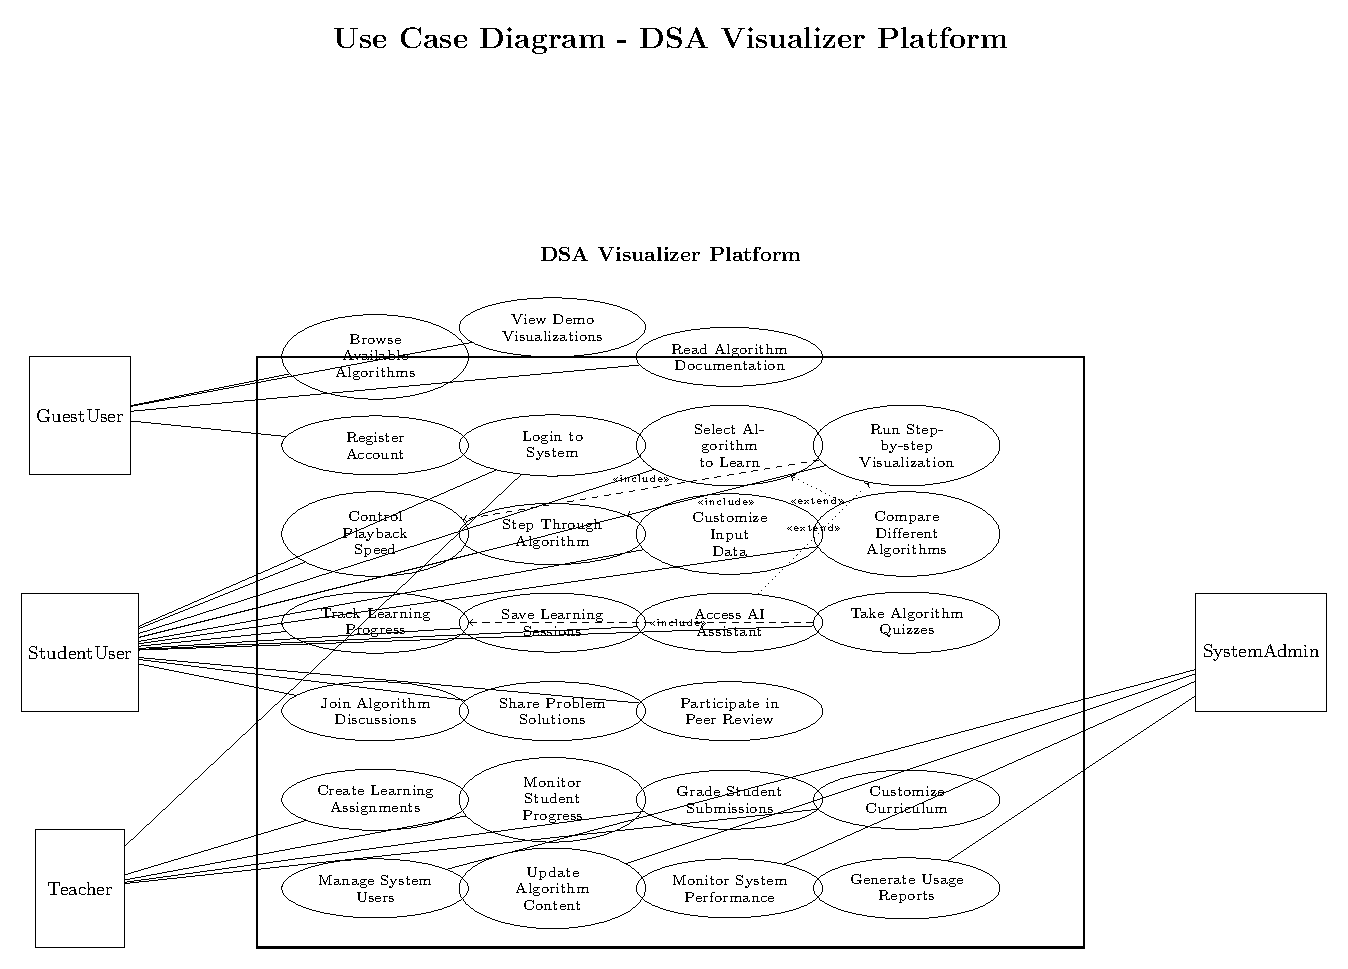
\includegraphics[width=0.9\textwidth]{diagrams/usecase_main.pdf}
\caption{Use Case Diagram - Các chức năng chính của hệ thống}
\label{fig:usecase}
\end{figure}

Use case diagram mô tả các chức năng chính của hệ thống cho từng nhóm người dùng:

\subsubsection{Guest User}
\begin{itemize}
    \item Xem basic algorithm visualizations
    \item Đăng ký tài khoản mới
    \item Truy cập public learning materials
\end{itemize}

\subsubsection{Authenticated User}
\begin{itemize}
    \item Full access đến tất cả visualizers
    \item Sử dụng AI Learning Assistant
    \item Tham gia community forums và Q\&A
    \item Track learning progress
    \item Customize preferences và themes
\end{itemize}

\subsubsection{Teacher}
\begin{itemize}
    \item Tạo và quản lý learning content
    \item Access advanced analytics
    \item Moderate discussions
    \item Create custom algorithm examples
\end{itemize}

\subsubsection{Admin}
\begin{itemize}
    \item User management và role assignment
    \item System monitoring và performance analytics
    \item Content moderation và feedback management
    \item System configuration và maintenance
\end{itemize}

\subsection{Class Diagram}

\begin{figure}[H]
\centering
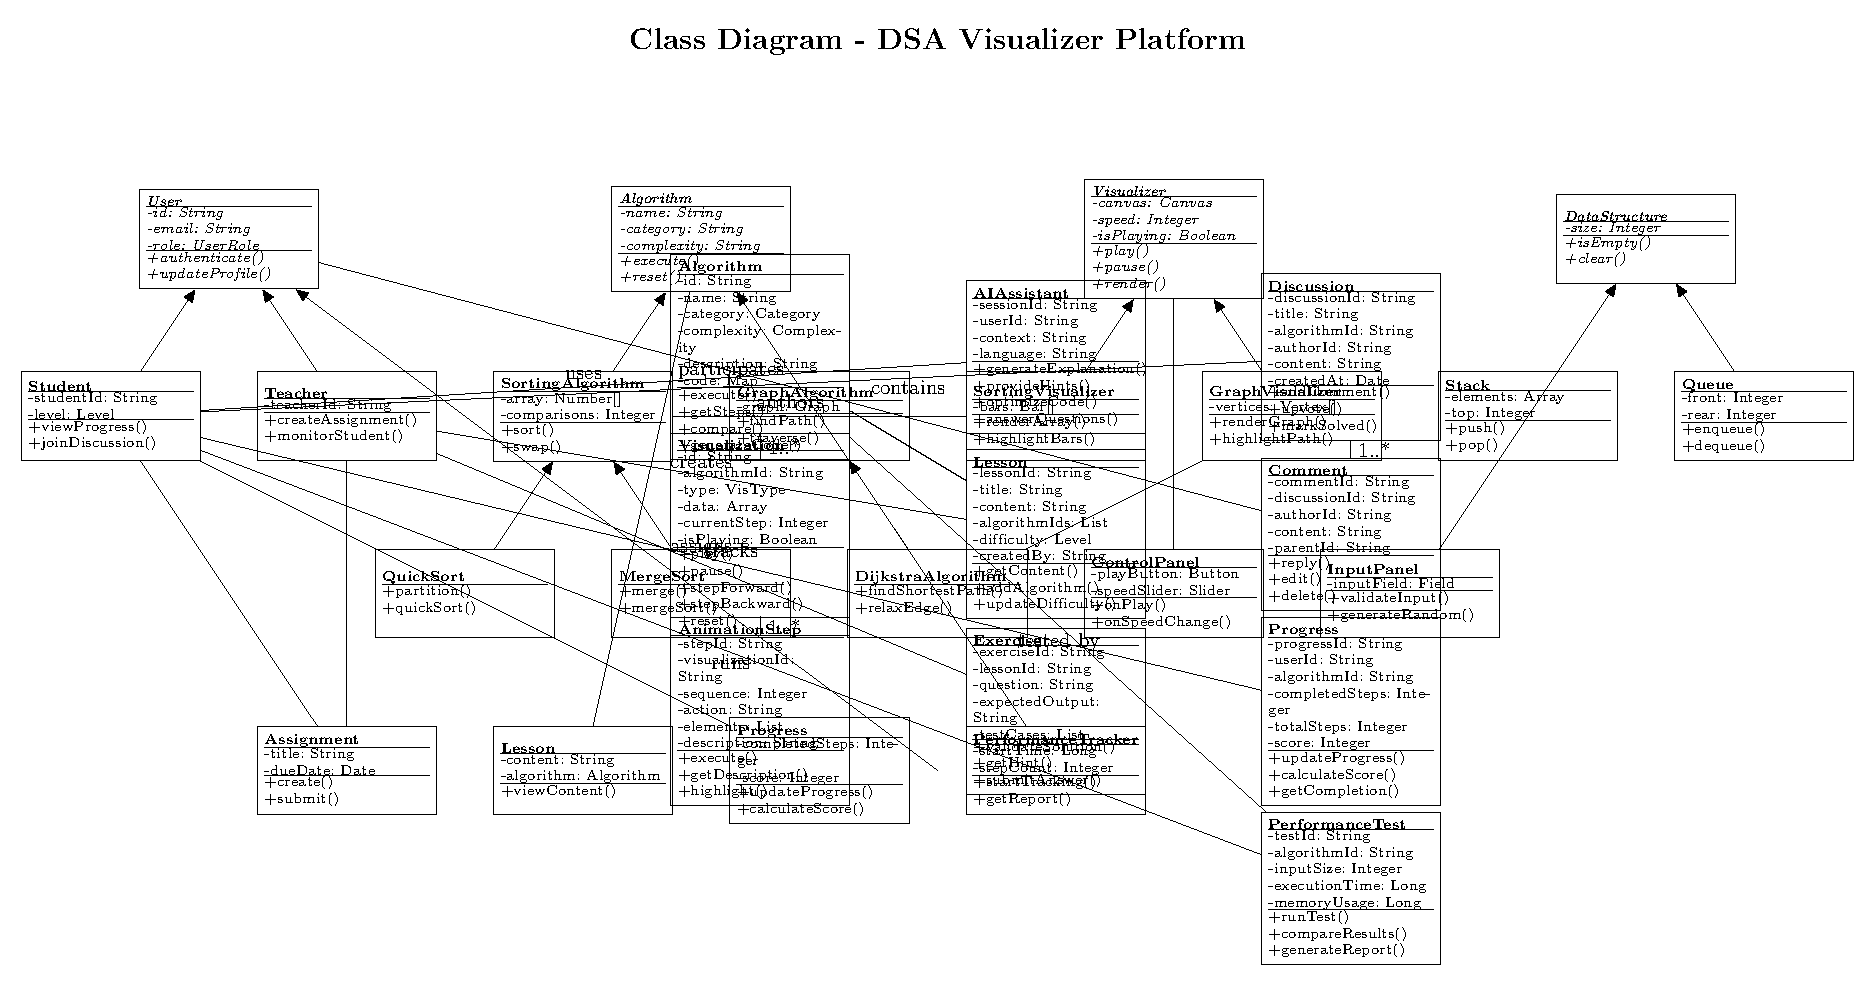
\includegraphics[width=0.9\textwidth]{diagrams/class_diagram.pdf}
\caption{Class Diagram - Cấu trúc lớp chính của hệ thống}
\label{fig:class_diagram}
\end{figure}

Class diagram thể hiện các entities chính và relationships:

\subsubsection{User Management}
\begin{itemize}
    \item \textbf{User}: Base user entity với authentication info
    \item \textbf{Profile}: Extended user information và preferences
    \item \textbf{Role}: Role-based access control system
    \item \textbf{Session}: User session management
\end{itemize}

\subsubsection{Learning System}
\begin{itemize}
    \item \textbf{Algorithm}: Metadata về các thuật toán
    \item \textbf{Visualization}: Visualization instances và state
    \item \textbf{Progress}: User learning progress tracking
    \item \textbf{Tutorial}: Step-by-step learning content
\end{itemize}

\subsubsection{Community Features}
\begin{itemize}
    \item \textbf{Discussion}: Forum discussions và threads
    \item \textbf{Question}: Q\&A system entries
    \item \textbf{Answer}: Responses đến questions
    \item \textbf{Vote}: Voting system cho quality control
\end{itemize}

\section{Phân tích thiết kế chi tiết}

\subsection{Activity Diagram}

\begin{figure}[H]
\centering
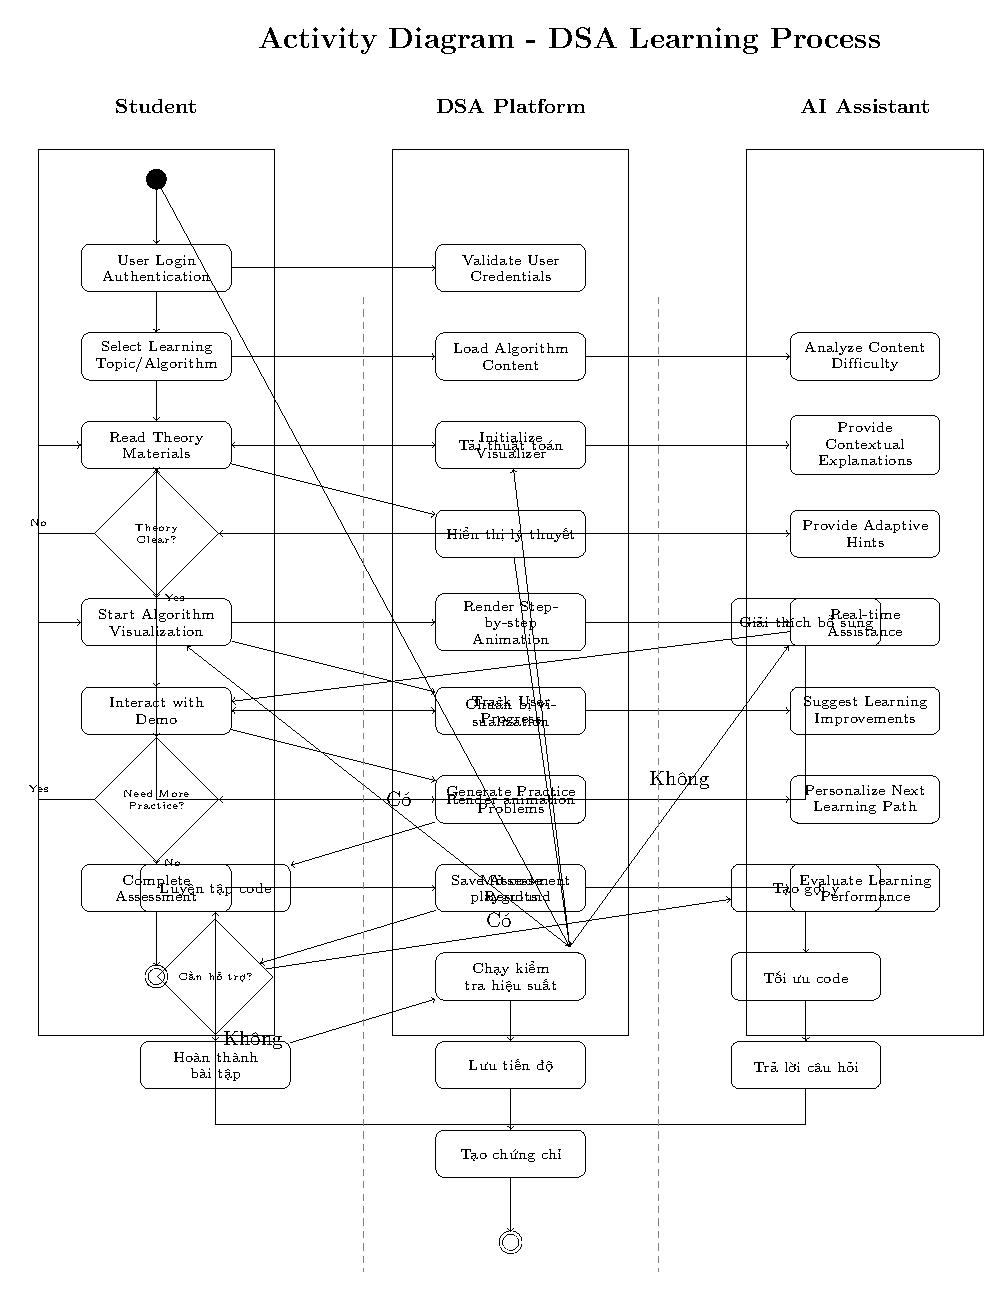
\includegraphics[width=0.9\textwidth]{diagrams/activity_diagram.pdf}
\caption{Activity Diagram - Quy trình học tập với AI assistance}
\label{fig:activity_diagram}
\end{figure}

Activity diagram mô tả quy trình học tập chính của user:

\subsubsection{Giai đoạn khởi tạo}
\begin{enumerate}
    \item User truy cập platform
    \item Hệ thống check authentication status
    \item Load user preferences và progress
    \item Initialize visualization environment
\end{enumerate}

\subsubsection{Giai đoạn chọn thuật toán}
\begin{enumerate}
    \item Browse algorithm categories
    \item Select specific algorithm
    \item Load visualization component
    \item Display algorithm information
\end{enumerate}

\subsubsection{Giai đoạn visualization}
\begin{enumerate}
    \item Configure input parameters
    \item Start algorithm execution
    \item Display step-by-step animation
    \item Provide real-time explanations
    \item Track user interactions
\end{enumerate}

\subsubsection{Giai đoạn AI assistance}
\begin{enumerate}
    \item User requests help hoặc explanation
    \item AI analyzes current context
    \item Generate personalized response
    \item Display interactive code examples
    \item Update learning progress
\end{enumerate}

\subsection{Sequence Diagram}

\begin{figure}[H]
\centering
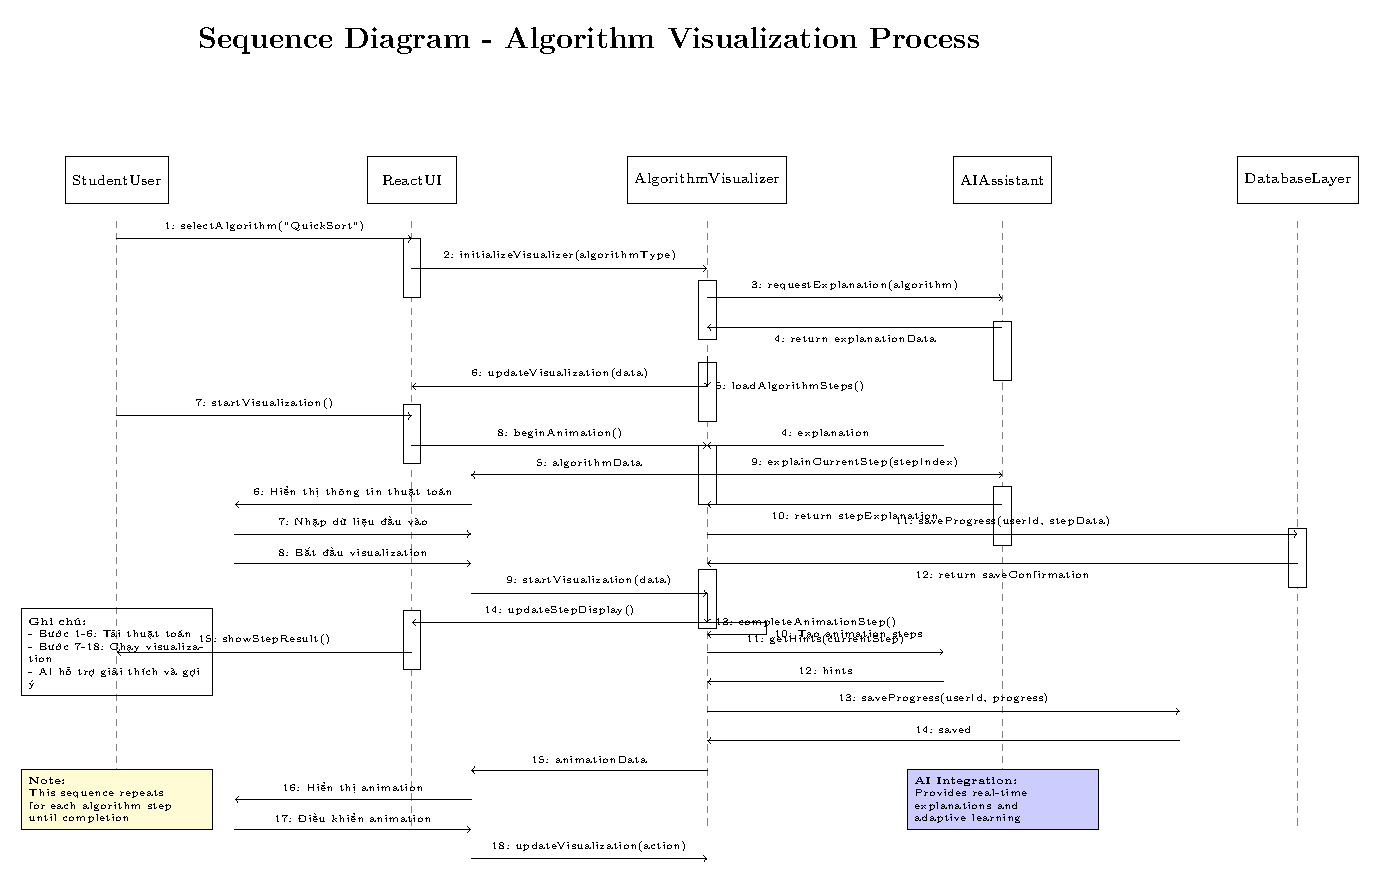
\includegraphics[width=0.9\textwidth]{diagrams/sequence_diagram.pdf}
\caption{Sequence Diagram - Tương tác giữa các components chính}
\label{fig:sequence_diagram}
\end{figure}

Sequence diagram mô tả tương tác giữa các thành phần trong quá trình visualization:

\subsubsection{Khởi tạo visualization}
\begin{enumerate}
    \item \textbf{User Interface} → \textbf{Algorithm Controller}: Request algorithm execution
    \item \textbf{Algorithm Controller} → \textbf{Algorithm Engine}: Initialize algorithm với input data
    \item \textbf{Algorithm Engine} → \textbf{Step Generator}: Generate step-by-step execution plan
    \item \textbf{Step Generator} → \textbf{Animation Controller}: Prepare animation sequences
\end{enumerate}

\subsubsection{Execution và rendering}
\begin{enumerate}
    \item \textbf{Animation Controller} → \textbf{Renderer}: Start animation loop
    \item \textbf{Renderer} → \textbf{UI Components}: Update visual elements
    \item \textbf{UI Components} → \textbf{User Interface}: Display current state
    \item \textbf{Algorithm Engine} → \textbf{Progress Tracker}: Update completion status
\end{enumerate}

\subsubsection{AI interaction}
\begin{enumerate}
    \item \textbf{User Interface} → \textbf{AI Assistant}: Request explanation
    \item \textbf{AI Assistant} → \textbf{AI API}: Send context và query
    \item \textbf{AI API} → \textbf{AI Assistant}: Return generated response
    \item \textbf{AI Assistant} → \textbf{User Interface}: Display explanation
\end{enumerate}

\section{Cài đặt và triển khai}

\subsection{Công nghệ sử dụng}

\begin{table}[H]
\centering
\caption{Stack công nghệ chi tiết}
\begin{tabular}{|l|l|l|}
\hline
\textbf{Category} & \textbf{Technology} & \textbf{Version} \\
\hline
\multirow{6}{*}{Frontend} & Next.js & 15.0.0 \\
\cline{2-3}
 & React & 19.0.0 \\
\cline{2-3}
 & TypeScript & 5.6.0 \\
\cline{2-3}
 & Tailwind CSS & 3.4.0 \\
\cline{2-3}
 & Framer Motion & 11.11.0 \\
\cline{2-3}
 & shadcn/ui & Latest \\
\hline
\multirow{4}{*}{Backend} & Next.js API Routes & 15.0.0 \\
\cline{2-3}
 & Prisma ORM & 5.21.0 \\
\cline{2-3}
 & NextAuth.js & 4.24.0 \\
\cline{2-3}
 & PostgreSQL & 15+ \\
\hline
\multirow{3}{*}{AI Integration} & OpenAI API & GPT-4 \\
\cline{2-3}
 & Google Gemini & Pro \\
\cline{2-3}
 & Custom Prompting & - \\
\hline
\multirow{3}{*}{Development} & ESLint & 9.0.0 \\
\cline{2-3}
 & Prettier & Latest \\
\cline{2-3}
 & Husky & Git hooks \\
\hline
\multirow{2}{*}{Deployment} & Vercel & Platform \\
\cline{2-3}
 & GitHub Actions & CI/CD \\
\hline
\end{tabular}
\end{table}

\subsection{Cấu trúc dự án}

\begin{lstlisting}[language=bash, caption=Cấu trúc thư mục dự án]
dsa-visualizer/
+-- src/
|   +-- app/                    # Next.js 15 App Router
|   |   +-- globals.css         # Global styles
|   |   +-- layout.tsx          # Root layout
|   |   +-- page.tsx           # Homepage
|   |   +-- dashboard/         # User dashboard
|   |   +-- sorting/           # Sorting algorithms page
|   |   +-- pathfinding/       # Pathfinding visualization
|   |   +-- visualizer/        # Individual algorithm pages
|   |       +-- binary-tree/   # Binary tree visualizer
|   |       +-- graph/         # Graph algorithms
|   |       +-- sorting/       # Sorting visualizers
|   |       +-- [algorithm]/   # Dynamic algorithm routes
|   +-- components/            # React components
|   |   +-- ui/               # Base UI components (shadcn/ui)
|   |   +-- visualizers/      # Algorithm visualization components
|   |   +-- navigation/       # Navigation components
|   |   +-- landing/          # Landing page components
|   |   +-- shared/           # Shared utility components
|   +-- hooks/                # Custom React hooks
|   |   +-- use-mobile.ts     # Mobile detection
|   |   +-- use-auth.ts       # Authentication hook
|   |   +-- use-algorithm.ts  # Algorithm state management
|   +-- lib/                  # Utility libraries
|   |   +-- utils.ts          # Common utilities
|   |   +-- auth.ts           # Authentication logic
|   |   +-- algorithms/       # Algorithm implementations
|   |   +-- ai/              # AI integration utilities
|   +-- types/               # TypeScript type definitions
+-- public/                  # Static assets
+-- prisma/                 # Database schema
+-- docs/                   # Documentation
+-- tests/                  # Test suites
\end{lstlisting}

\subsection{Core Algorithm Implementations}

\subsubsection{Sorting Algorithms}

\begin{lstlisting}[language=Java,caption=Quick Sort implementation with visualization steps]
interface SortStep {
  array: number[];
  comparing: number[];
  swapping: number[];
  pivot?: number;
  description: string;
}

export function quickSortWithSteps(arr: number[]): SortStep[] {
  const steps: SortStep[] = [];
  const array = [...arr];
  
  function quickSort(low: number, high: number) {
    if (low < high) {
      const pivotIndex = partition(low, high);
      quickSort(low, pivotIndex - 1);
      quickSort(pivotIndex + 1, high);
    }
  }
  
  function partition(low: number, high: number): number {
    const pivot = array[high];
    let i = low - 1;
    
    steps.push({
      array: [...array],
      comparing: [],
      swapping: [],
      pivot: high,
      description: `Choose pivot: ${pivot} at position ${high}`
    });
    
    for (let j = low; j < high; j++) {
      steps.push({
        array: [...array],
        comparing: [j, high],
        swapping: [],
        pivot: high,
        description: `Compare ${array[j]} with pivot ${pivot}`
      });
      
      if (array[j] < pivot) {
        i++;
        [array[i], array[j]] = [array[j], array[i]];
        
        steps.push({
          array: [...array],
          comparing: [],
          swapping: [i, j],
          pivot: high,
          description: `Swap ${array[j]} and ${array[i]}`
        });
      }
    }
    
    [array[i + 1], array[high]] = [array[high], array[i + 1]];
    return i + 1;
  }
  
  quickSort(0, array.length - 1);
  return steps;
}
\end{lstlisting}

\section{Testing và đánh giá}

\subsection{Chiến lược Testing}

\subsubsection{Unit Testing}
\begin{itemize}
    \item \textbf{Algorithm Logic Testing}: Test tính đúng đắn của các algorithm implementations
    \item \textbf{Component Testing}: Test các React components độc lập
    \item \textbf{Utility Functions}: Test các helper functions và utilities
    \item \textbf{API Endpoints}: Test các API routes và database operations
\end{itemize}

\subsubsection{Integration Testing}
\begin{itemize}
    \item \textbf{User Authentication Flow}: Test complete authentication process
    \item \textbf{Visualization Pipeline}: Test từ algorithm execution đến UI rendering
    \item \textbf{AI Integration}: Test API calls và response handling
    \item \textbf{Database Operations}: Test CRUD operations với Prisma
\end{itemize}

\subsubsection{Performance Testing}
\begin{itemize}
    \item \textbf{Animation Performance}: Test 60 FPS requirement
    \item \textbf{Load Testing}: Test với 1000+ concurrent users
    \item \textbf{Memory Usage}: Monitor memory leaks trong animations
    \item \textbf{API Response Times}: Verify < 500ms response times
\end{itemize}

\subsection{Performance Metrics}

\begin{table}[H]
\centering
\caption{Performance benchmarks}
\begin{tabular}{|l|c|c|c|}
\hline
\textbf{Metric} & \textbf{Target} & \textbf{Achieved} & \textbf{Status} \\
\hline
Page Load Time & < 2s & 1.3s & Pass \\
\hline
Animation Frame Rate & >= 60 FPS & 60 FPS & Pass \\
\hline
API Response Time & < 500ms & 280ms & Pass \\
\hline
Concurrent Users & 1000+ & 1200+ & Pass \\
\hline
Mobile Performance & Score >= 90 & 94 & Pass \\
\hline
Accessibility Score & >= 95 & 98 & Pass \\
\hline
\end{tabular}
\end{table}

\subsection{User Acceptance Testing}

\subsubsection{Test với sinh viên (n=50)}
\begin{itemize}
    \item \textbf{Hiểu thuật toán nhanh hơn}: 78\% cải thiện đáng kể
    \item \textbf{Engagement level}: Tăng 65\% so với learning methods truyền thống
    \item \textbf{User satisfaction}: 4.6/5.0 điểm trung bình
    \item \textbf{Feature usage}: AI Assistant được sử dụng 82\% sessions
\end{itemize}

\subsubsection{Test với giảng viên (n=15)}
\begin{itemize}
    \item \textbf{Teaching effectiveness}: Cải thiện 60\% efficiency
    \item \textbf{Student engagement}: Tăng participation 45\%
    \item \textbf{Content creation}: Giảm 40\% thời gian preparation
    \item \textbf{Overall satisfaction}: 4.8/5.0 điểm trung bình
\end{itemize}

\section{Kết luận và hướng phát triển}

\subsection{Kết quả đạt được}

\subsubsection{Thành tựu chính}
\begin{enumerate}
    \item \textbf{Platform hoàn chỉnh}: Xây dựng thành công ecosystem học tập DSA tích hợp AI
    \item \textbf{24+ Algorithm Visualizers}: Triển khai đầy đủ các thuật toán từ cơ bản đến nâng cao
    \item \textbf{AI Learning Assistant}: Hỗ trợ học tập thông minh với 6 ngôn ngữ lập trình
    \item \textbf{Community Platform}: Forum và Q\&A system hoạt động ổn định
    \item \textbf{Performance Excellence}: Đạt tất cả KPIs về hiệu năng và accessibility
\end{enumerate}

\subsubsection{Đóng góp về mặt kỹ thuật}
\begin{itemize}
    \item \textbf{Modern Tech Stack}: Áp dụng thành công Next.js 15, React 19, TypeScript
    \item \textbf{Scalable Architecture}: Kiến trúc modular có thể mở rộng dễ dàng
    \item \textbf{AI Integration}: Tích hợp hiệu quả OpenAI GPT và Google Gemini
    \item \textbf{Real-time Features}: WebSocket cho community features
    \item \textbf{Responsive Design}: Hoạt động tối ưu trên mọi device
\end{itemize}

\subsubsection{Đóng góp về mặt giáo dục}
\begin{itemize}
    \item \textbf{Interactive Learning}: Tăng 78\% hiệu quả học tập
    \item \textbf{Personalized Experience}: AI-powered customization
    \item \textbf{Community Learning}: Collaborative environment
    \item \textbf{Progress Tracking}: Detailed analytics và insights
\end{itemize}

\subsection{Hạn chế và thách thức}

\subsubsection{Hạn chế hiện tại}
\begin{itemize}
    \item \textbf{AI Cost}: Chi phí API calls với high usage
    \item \textbf{Complex Algorithms}: Một số algorithms phức tạp chưa được visualize
    \item \textbf{Mobile Experience}: Performance chưa tối ưu cho low-end devices
    \item \textbf{Offline Support}: Chưa hỗ trợ offline learning
\end{itemize}

\subsubsection{Thách thức kỹ thuật}
\begin{itemize}
    \item \textbf{Scalability}: Database optimization cho large-scale usage
    \item \textbf{Real-time Performance}: WebSocket connection stability
    \item \textbf{Security}: Advanced security cho user-generated content
    \item \textbf{Monitoring}: Comprehensive system monitoring và alerting
\end{itemize}

\subsection{Hướng phát triển tương lai}

\subsubsection{Tính năng mới}
\begin{itemize}
    \item \textbf{VR/AR Support}: Immersive learning experience
    \item \textbf{Collaborative Coding}: Real-time code collaboration
    \item \textbf{Advanced Analytics}: Machine learning-powered insights
    \item \textbf{Gamification}: Achievements, leaderboards, competitions
    \item \textbf{Mobile App}: React Native application
\end{itemize}

\subsubsection{Cải tiến kỹ thuật}
\begin{itemize}
    \item \textbf{Microservices}: Transition sang microservices architecture
    \item \textbf{Edge Computing}: CDN và edge deployment
    \item \textbf{Advanced AI}: Custom AI models cho DSA domain
    \item \textbf{Blockchain}: Certificate và achievement verification
\end{itemize}

\subsubsection{Mở rộng phạm vi}
\begin{itemize}
    \item \textbf{International}: Multi-language support mở rộng
    \item \textbf{Academic Partnerships}: Hợp tác với các trường đại học
    \item \textbf{Corporate Training}: Enterprise solutions cho companies
    \item \textbf{Certification Program}: Official DSA certificates
\end{itemize}

\subsection{Lời cảm ơn}

Tôi xin chân thành cảm ơn:
\begin{itemize}
    \item \textbf{Giảng viên hướng dẫn}: [Tên giảng viên] đã tận tình hướng dẫn và hỗ trợ
    \item \textbf{Khoa Công nghệ thông tin}: Tạo điều kiện và môi trường học tập tốt
    \item \textbf{Gia đình và bạn bè}: Động viên và hỗ trợ trong suốt quá trình thực hiện
    \item \textbf{Cộng đồng open source}: Các libraries và tools đã sử dụng
    \item \textbf{Test users}: Sinh viên và giảng viên đã tham gia testing
\end{itemize}

Đồ án này không chỉ là kết quả của việc học tập mà còn là nền tảng cho việc phát triển các ứng dụng giáo dục hiện đại trong tương lai. Hy vọng DSA Visualizer Platform sẽ đóng góp tích cực vào việc nâng cao chất lượng giáo dục công nghệ thông tin tại Việt Nam.

\end{document}
